\documentclass[a5paper, 10pt]{article}

% ============================================================
% Algoritmos e Estruturas de Dados em C++ (TecPro Tecnologias)
% Mesmo modelo do livro "Node.js, Express e MySQL": cada capítulo fica em
% capitulos/capitulo-NN.tex e vira página do site com
% site/ferramentas/converter_latex.py (modelo "livro").
% ============================================================
\usepackage[utf8]{inputenc}
\usepackage[T1]{fontenc}
\usepackage[portuguese]{babel}
\usepackage{geometry}
\usepackage{graphicx}
\usepackage{tikz}
\usetikzlibrary{arrows.meta, positioning, shapes.geometric, calc}
\usepackage[table]{xcolor}

% Cores do logo da TecPro
\definecolor{navy}{RGB}{23,45,80}
\definecolor{laranja}{RGB}{250,110,29}
\definecolor{cinzalogo}{RGB}{107,114,126}
\usepackage{booktabs}
\usepackage{longtable}
\usepackage{enumitem}
\usepackage{hyperref}
\hypersetup{hidelinks}
\usepackage{parskip}
\usepackage{fvextra}
\usepackage{array}
\usepackage{amsmath}

\setlength{\emergencystretch}{2.5em}
\AtBeginDocument{\renewcommand{\contentsname}{Sumário}}

\geometry{
  a5paper,
  twoside,
  bindingoffset=8mm,
  inner=16mm,
  outer=12mm,
  top=15mm,
  bottom=18mm
}

% os títulos já trazem a numeração ("Capítulo 1 -- ...", "1.1 ...")
\setcounter{secnumdepth}{0}

\definecolor{headergray}{HTML}{1F2937}
\definecolor{rowgray}{HTML}{E5E7EB}
\definecolor{boxgray}{HTML}{F3F4F6}
\definecolor{borderblack}{HTML}{111111}

\newcommand{\tblheader}[1]{\textcolor{white}{\textbf{#1}}}

\newenvironment{destaque}[1]
  {\par\noindent\textbf{#1}\par\vspace{2pt}\hrule\vspace{6pt}}
  {\par\vspace{6pt}\hrule\vspace{10pt}}

\usepackage{tcolorbox}
\tcbuselibrary{skins,breakable}

\newtcolorbox{codigo}{
  colback=boxgray,
  colframe=borderblack,
  boxrule=0.4pt,
  arc=1.5mm,
  left=6pt, right=6pt, top=5pt, bottom=5pt,
  fontupper=\ttfamily\footnotesize,
  breakable
}

\begin{document}

% ============================================================
% CAPA
% ============================================================
\begin{titlepage}
\centering

\vspace*{1.1cm}


\includegraphics[width=2.3cm]{icone_tecpro.png}

\vspace{0.3cm}

{\Large \textbf{\textcolor{navy}{Tec}\textcolor{laranja}{Pro}}}\\[1pt]
{\footnotesize \textcolor{cinzalogo}{T E C N O L O G I A S}}

\vspace{0.2cm}

{\footnotesize \textcolor{cinzalogo}{Desenvolvimento, Apostilas e Cursos Online}}

\vspace{1cm}

% ícones genéricos dos temas do livro
\begin{tikzpicture}[baseline]

  % --- C++ ---
  \begin{scope}[shift={(0,0)}]
    \node[font=\Large\bfseries, text=navy] at (0,0.15) {C++};
    \node[font=\tiny, text=cinzalogo] at (0,-0.55) {Linguagem};
  \end{scope}

  % --- Lista encadeada: três nós ligados ---
  \begin{scope}[shift={(2.5,0)}]
    \foreach \x in {-0.6,0,0.6} {
      \draw[navy, line width=1pt, fill=laranja!12] (\x-0.2,0) rectangle (\x+0.2,0.3);
    }
    \draw[-{Stealth}, navy, line width=0.8pt] (-0.4,0.15) -- (-0.2,0.15);
    \draw[-{Stealth}, navy, line width=0.8pt] (0.2,0.15) -- (0.4,0.15);
    \node[font=\tiny, text=cinzalogo] at (0,-0.55) {Listas};
  \end{scope}

  % --- Árvore binária ---
  \begin{scope}[shift={(5.0,0)}]
    \draw[navy, line width=1pt] (0,0.45) -- (-0.35,0.0) (0,0.45) -- (0.35,0.0);
    \foreach \p in {(0,0.45),(-0.35,0.0),(0.35,0.0)} {
      \filldraw[draw=navy, line width=1pt, fill=laranja!12] \p circle (0.12);
    }
    \node[font=\tiny, text=cinzalogo] at (0,-0.55) {Árvores};
  \end{scope}

  % --- Complexidade ---
  \begin{scope}[shift={(7.5,0)}]
    \node[font=\Large\bfseries, text=navy] at (0,0.15) {$O(n)$};
    \node[font=\tiny, text=cinzalogo] at (0,-0.55) {Complexidade};
  \end{scope}

\end{tikzpicture}

\vspace{1.3cm}

\begin{tikzpicture}[remember picture, overlay]
  \fill[navy] (current page.south west) rectangle
    ($(current page.south east)!0.32!(current page.north east)$);
  \draw[laranja, line width=3.2pt]
    ($(current page.south west)!0.32!(current page.north west)$) --
    ($(current page.south east)!0.32!(current page.north east)$);
  \begin{scope}[opacity=0.16]
    \draw[laranja, line width=5mm, line cap=round]
      ($(current page.south east)+(-14mm,10mm)$) --
      ($(current page.south east)+(-6mm,17mm)$) --
      ($(current page.south east)+(-14mm,24mm)$);
  \end{scope}
  \node[align=center, text width=0.84\paperwidth] at
    ($(current page.south west)!0.20!(current page.north west)+(0.5\paperwidth,0)$)
    {\color{white}\LARGE\bfseries Algoritmos e Estruturas de Dados};
  \node[align=center, text width=0.78\paperwidth] at
    ($(current page.south west)!0.08!(current page.north west)+(0.5\paperwidth,0)$)
    {\color{laranja}\normalsize Em C++, com comparações em Python};
\end{tikzpicture}

\vfill

\end{titlepage}

% ============================================================
% FICHA TÉCNICA
% ============================================================
\thispagestyle{empty}
\vspace*{\fill}

\begin{center}
{\large \textbf{Algoritmos e Estruturas de Dados}}\\[2pt]
{\small Em C++, com comparações em Python}

\vspace{1cm}

\rule{3cm}{0.4pt}

\vspace{0.4cm}

\textbf{TecPro Tecnologias}\\
{\footnotesize Desenvolvimento, Apostilas e Cursos Online}

\vspace{0.5cm}

{\footnotesize 2026}
\end{center}

\vspace*{\fill}

\noindent\footnotesize Todos os direitos reservados. Nenhuma parte desta publicação pode ser reproduzida, armazenada ou transmitida de qualquer forma, ou por qualquer meio, sem autorização prévia da TecPro Tecnologias.

\newpage

\tableofcontents
\newpage

% ============================================================
% CAPÍTULOS
% ============================================================
\section{Capítulo 1 -- Fundamentos de C++ para Estruturas de Dados}

Em Algoritmos I você aprendeu a base da programação: variáveis, tipos e operadores, condicionais e laços, funções, strings, vetores e matrizes. Também conheceu, de forma introdutória, listas, pilhas, filas, busca, ordenação e recursão. Agora vamos aprofundar: construir essas estruturas por dentro, de forma eficiente, e analisar o custo de cada operação.

Para isso, você precisa de algumas ferramentas do C++ que as estruturas de dados usam o tempo todo. Este capítulo faz duas coisas:

\begin{itemize}
  \item \textbf{retoma rapidamente} o que você já conhece, agora escrito em C++: estrutura de um programa, tipos, vetores e funções (seções 1.2 a 1.4);
  \item \textbf{apresenta o que é novo} e indispensável daqui em diante: ponteiros, memória dinâmica, structs, classes e templates (seções 1.5 a 1.9).
\end{itemize}

Se você já se sente seguro com a primeira parte, pode passar por ela rapidamente. A segunda parte merece atenção total: é a base de todos os capítulos seguintes.

\subsection{1.1 Por que estudar estruturas de dados em C++?}

Em linguagens como Python, Java ou JavaScript, a memória é administrada automaticamente. Você cria uma lista, adiciona elementos e nunca precisa pensar onde eles estão guardados. Isso é ótimo para produtividade, mas esconde justamente o que queremos entender nesta disciplina: \textbf{como os dados são organizados na memória}.

Em C++, você enxerga e controla essa organização. Uma lista encadeada deixa de ser uma caixa-preta e passa a ser o que ela realmente é: um conjunto de blocos de memória, cada um apontando para o próximo. Quando você entende isso, passa a entender também por que uma operação é rápida ou lenta, e esse é o centro da análise de algoritmos.

Ao longo da apostila, sempre que ajudar a entender um conceito, vamos mostrar como a mesma ideia aparece em Python. Assim você vê as duas faces da moeda: o que acontece \textit{por dentro} (C++) e como isso costuma ficar \textit{escondido} em uma linguagem de mais alto nível (Python).

\subsection{1.2 Estrutura de um programa em C++}

Todo programa em C++ começa a ser executado pela função \texttt{main}. Veja um programa completo:

\begin{codigo}
\begin{Verbatim}[breaklines=true, breaksymbolleft={}, fontsize=\footnotesize]
#include <iostream>   // biblioteca de entrada e saída (cin, cout)
using namespace std;  // permite escrever cout em vez de std::cout

int main() {
    int idade;
    cout << "Digite sua idade: ";
    cin >> idade;                       // lê um valor do teclado
    cout << "Daqui a 10 anos voce tera " << idade + 10 << " anos" << endl;
    return 0;                           // 0 indica que terminou sem erro
}
\end{Verbatim}
\end{codigo}

Alguns pontos importantes:

\begin{itemize}
  \item \texttt{\#include} traz uma biblioteca para o programa. A \texttt{iostream} oferece \texttt{cin} (entrada) e \texttt{cout} (saída).
  \item Todo comando termina com \texttt{;} e todo bloco fica entre \texttt{\{} e \texttt{\}}.
  \item C++ diferencia letras maiúsculas de minúsculas: \texttt{idade} e \texttt{Idade} são variáveis diferentes.
  \item O programa precisa ser \textbf{compilado} antes de rodar. Com o compilador g++, por exemplo: \texttt{g++ programa.cpp -o programa}.
\end{itemize}

\begin{destaque}{Comparando com Python}
Em Python, o mesmo programa não precisa de \texttt{main}, de tipos nem de compilação, porque é interpretado linha a linha:

\begin{codigo}
\begin{Verbatim}[breaklines=true, breaksymbolleft={}, fontsize=\footnotesize]
idade = int(input("Digite sua idade: "))
print(f"Daqui a 10 anos voce tera {idade + 10} anos")
\end{Verbatim}
\end{codigo}

Em C++, o compilador verifica os tipos antes de o programa rodar. Muitos erros que em Python só aparecem durante a execução, em C++ aparecem já na compilação.
\end{destaque}

\subsection{1.3 Tipos, variáveis e vetores}

Uma variável é um espaço na memória com um nome e um tipo. O tipo define quanto espaço ela ocupa e que valores pode guardar.

\begin{center}
\begin{tabular}{@{}p{0.22\linewidth}p{0.36\linewidth}p{0.28\linewidth}@{}}
\toprule
\rowcolor{headergray}
\tblheader{Tipo} & \tblheader{Guarda} & \tblheader{Exemplo} \\
\midrule
\texttt{int} & números inteiros & \texttt{int qtd = 10;} \\
\rowcolor{rowgray} \texttt{double} & números com casas decimais & \texttt{double nota = 8.5;} \\
\texttt{char} & um caractere & \texttt{char letra = 'A';} \\
\rowcolor{rowgray} \texttt{bool} & verdadeiro ou falso & \texttt{bool ok = true;} \\
\texttt{string} & texto (precisa de \texttt{<string>}) & \texttt{string nome = "Ana";} \\
\bottomrule
\end{tabular}
\end{center}

Um \textbf{vetor} (array) guarda vários valores do mesmo tipo, um ao lado do outro na memória. Os índices começam em 0:

\begin{codigo}
\begin{Verbatim}[breaklines=true, breaksymbolleft={}, fontsize=\footnotesize]
int notas[5] = {7, 9, 6, 10, 8};   // 5 inteiros seguidos na memória

for (int i = 0; i < 5; i++) {
    cout << "Nota " << i << ": " << notas[i] << endl;
}
\end{Verbatim}
\end{codigo}

O vetor tem uma limitação que vai motivar vários capítulos desta apostila: o \textbf{tamanho é fixo}. Se você declarou espaço para 5 notas e chegou uma sexta, não há onde colocá-la. Inserir um elemento no meio também é trabalhoso, porque todos os seguintes precisam ser deslocados uma posição. As estruturas que vamos construir, como as listas encadeadas, existem justamente para contornar essas limitações.

\subsection{1.4 Funções e passagem de parâmetros}

Uma função é um trecho de código com nome, que recebe dados (parâmetros), faz um trabalho e pode devolver um resultado. Funções evitam repetir código e deixam o programa mais fácil de ler e de manter.

\begin{codigo}
\begin{Verbatim}[breaklines=true, breaksymbolleft={}, fontsize=\footnotesize]
// recebe os três coeficientes e diz se a equação tem raízes reais
bool temRaizReal(double a, double b, double c) {
    double delta = b * b - 4 * a * c;
    return delta >= 0;
}

// void: a função não devolve valor, só executa uma ação
void imprimirVetor(int v[], int tamanho) {
    for (int i = 0; i < tamanho; i++) {
        cout << v[i] << " ";
    }
    cout << endl;
}
\end{Verbatim}
\end{codigo}

O ponto mais importante para esta apostila é \textbf{como os parâmetros chegam à função}. Em C++ há três formas.

\subsubsection{Por valor: a função recebe uma cópia}

\begin{codigo}
\begin{Verbatim}[breaklines=true, breaksymbolleft={}, fontsize=\footnotesize]
void dobrar(int x) {
    x = x * 2;          // altera só a cópia
}

int main() {
    int n = 5;
    dobrar(n);
    cout << n << endl;  // imprime 5: o n original não mudou
}
\end{Verbatim}
\end{codigo}

\subsubsection{Por referência: a função trabalha na variável original}

Basta acrescentar \texttt{\&} depois do tipo do parâmetro. A função passa a usar a própria variável de quem chamou, sem cópia:

\begin{codigo}
\begin{Verbatim}[breaklines=true, breaksymbolleft={}, fontsize=\footnotesize]
void dobrar(int &x) {
    x = x * 2;          // altera a variável original
}

void trocar(int &a, int &b) {
    int auxiliar = a;
    a = b;
    b = auxiliar;
}

int main() {
    int n = 5;
    dobrar(n);
    cout << n << endl;  // imprime 10

    int p = 1, q = 2;
    trocar(p, q);
    cout << p << " " << q << endl;  // imprime 2 1
}
\end{Verbatim}
\end{codigo}

\subsubsection{Por referência constante: sem cópia e sem alteração}

Quando o dado é grande (um texto longo, um vetor de milhares de itens) e a função só precisa ler, use \texttt{const}~\texttt{\&}. Você evita a cópia, que custa tempo e memória, e o compilador garante que a função não altera o original:

\begin{codigo}
\begin{Verbatim}[breaklines=true, breaksymbolleft={}, fontsize=\footnotesize]
#include <string>

int contarVogais(const string &texto) {
    int total = 0;
    for (char c : texto) {
        if (c == 'a' || c == 'e' || c == 'i' || c == 'o' || c == 'u') {
            total++;
        }
    }
    return total;
}
\end{Verbatim}
\end{codigo}

\begin{destaque}{Comparando com Python}
Python não deixa você escolher. Números e textos se comportam como se fossem passados por valor, porque não podem ser alterados (são \textit{imutáveis}). Já listas e dicionários são passados de forma que a função pode modificá-los:

\begin{codigo}
\begin{Verbatim}[breaklines=true, breaksymbolleft={}, fontsize=\footnotesize]
def dobrar(x):
    x = x * 2          # cria um novo número só dentro da função

def adicionar(lista):
    lista.append(99)   # modifica a lista original

n = 5
dobrar(n)
print(n)       # 5

numeros = [1, 2]
adicionar(numeros)
print(numeros) # [1, 2, 99]
\end{Verbatim}
\end{codigo}

Em C++ essa decisão é sua e fica escrita na assinatura da função, o que torna o comportamento explícito.
\end{destaque}

\subsection{1.5 Ponteiros}

Toda variável ocupa uma posição na memória, e cada posição tem um \textbf{endereço}, como o número de uma casa em uma rua. Um \textbf{ponteiro} é uma variável que guarda um endereço: em vez de guardar um valor, ele aponta para onde o valor está.

Dois operadores fazem todo o trabalho:

\begin{itemize}
  \item \texttt{\&variavel} devolve o \textbf{endereço} da variável;
  \item \texttt{*ponteiro} acessa o \textbf{valor} que está no endereço guardado (isso se chama \textit{desreferenciar}).
\end{itemize}

\begin{codigo}
\begin{Verbatim}[breaklines=true, breaksymbolleft={}, fontsize=\footnotesize]
int idade = 20;
int *p = &idade;      // p guarda o endereço de idade

cout << idade << endl;  // 20
cout << p << endl;      // um endereço, por exemplo 0x61fe14
cout << *p << endl;     // 20: o valor que está no endereço

*p = 21;                // altera idade através do ponteiro
cout << idade << endl;  // 21
\end{Verbatim}
\end{codigo}

Uma forma de visualizar o que aconteceu na memória:

\begin{center}
\begin{tabular}{@{}p{0.22\linewidth}p{0.26\linewidth}p{0.36\linewidth}@{}}
\toprule
\rowcolor{headergray}
\tblheader{Variável} & \tblheader{Endereço} & \tblheader{Conteúdo} \\
\midrule
\texttt{idade} & \texttt{0x61fe14} & \texttt{21} \\
\rowcolor{rowgray} \texttt{p} & \texttt{0x61fe18} & \texttt{0x61fe14} (aponta para \texttt{idade}) \\
\bottomrule
\end{tabular}
\end{center}

Um ponteiro que não aponta para nada deve valer \texttt{nullptr}. Você vai usar muito esse valor: é ele que marca o fim de uma lista encadeada ou um galho vazio de uma árvore. Antes de desreferenciar um ponteiro, verifique se ele não é nulo:

\begin{codigo}
\begin{Verbatim}[breaklines=true, breaksymbolleft={}, fontsize=\footnotesize]
int *q = nullptr;   // não aponta para nada

if (q != nullptr) {
    cout << *q << endl;  // só acessa se for seguro
}
\end{Verbatim}
\end{codigo}

\begin{destaque}{Referência ou ponteiro?}
Os dois permitem trabalhar com a variável original, mas têm diferenças. Uma \textbf{referência} (\texttt{int \&r = x;}) é um apelido: precisa nascer ligada a uma variável e nunca muda de alvo. Um \textbf{ponteiro} pode começar vazio (\texttt{nullptr}) e pode passar a apontar para outro lugar. Por isso as estruturas de dados usam ponteiros: um nó de uma lista precisa poder apontar para \textit{nenhum} nó, ou mudar de vizinho quando você insere ou remove elementos.
\end{destaque}

\subsection{1.6 Memória dinâmica: new e delete}

As variáveis declaradas dentro de uma função ficam em uma área chamada \textbf{pilha de execução} (\textit{stack}). Elas são criadas quando a função começa e destruídas automaticamente quando ela termina. Isso é prático, mas tem um limite: você não consegue criar, durante a execução, quantos elementos quiser e mantê-los vivos depois que a função acabar.

Para isso existe a memória dinâmica, ou \textbf{heap}. Com \texttt{new}, você pede ao sistema um espaço que continua existindo até você mesmo liberá-lo com \texttt{delete}:

\begin{codigo}
\begin{Verbatim}[breaklines=true, breaksymbolleft={}, fontsize=\footnotesize]
int *p = new int;     // reserva espaço para um int no heap
*p = 42;
cout << *p << endl;   // 42
delete p;             // devolve o espaço
p = nullptr;          // boa prática: não deixar o endereço antigo

// vetor com tamanho decidido durante a execução
int n;
cout << "Quantos valores? ";
cin >> n;
int *valores = new int[n];   // n inteiros no heap
for (int i = 0; i < n; i++) {
    valores[i] = i * i;
}
delete[] valores;            // vetor: libera com delete[]
\end{Verbatim}
\end{codigo}

Toda estrutura de dados dinâmica desta apostila funciona assim: cada novo elemento é criado com \texttt{new} e, quando sai da estrutura, é liberado com \texttt{delete}.

\begin{destaque}{Regra de ouro da memória dinâmica}
Para cada \texttt{new} deve existir exatamente um \texttt{delete} (e para cada \texttt{new[]}, um \texttt{delete[]}). Se você esquecer o \texttt{delete}, o espaço fica preso até o programa terminar: é o chamado \textbf{vazamento de memória} (\textit{memory leak}). Se fizer \texttt{delete} duas vezes, ou usar o ponteiro depois do \texttt{delete}, o comportamento é imprevisível e o programa pode travar.
\end{destaque}

\begin{destaque}{Comparando com Python}
Em Python não existe \texttt{delete} para liberar memória. O próprio interpretador percebe quando um objeto não é mais usado por ninguém e o remove: é a \textbf{coleta de lixo} (\textit{garbage collection}). Isso evita vazamentos e ponteiros inválidos, mas tem um custo: você perde o controle de quando a memória é liberada e de quanto espaço cada estrutura realmente ocupa.
\end{destaque}

\subsection{1.7 Structs: agrupando dados}

Uma \texttt{struct} junta vários dados relacionados em um único tipo novo. Em vez de ter variáveis soltas para nome, idade e matrícula de um aluno, você cria o tipo \texttt{Aluno}:

\begin{codigo}
\begin{Verbatim}[breaklines=true, breaksymbolleft={}, fontsize=\footnotesize]
struct Aluno {
    string nome;
    int matricula;
    double media;
};

int main() {
    Aluno a;
    a.nome = "Ana";          // o ponto acessa cada campo
    a.matricula = 2026001;
    a.media = 8.7;

    Aluno *p = &a;
    cout << p->nome << endl; // com ponteiro, usa-se a seta ->
}
\end{Verbatim}
\end{codigo}

Repare no operador \texttt{->}: quando você tem um \textbf{ponteiro} para uma struct, \texttt{p->nome} é o mesmo que \texttt{(*p).nome}. Ele vai aparecer em praticamente todo o código dos próximos capítulos.

\subsubsection{Uma prévia: o nó de uma lista encadeada}

Uma struct pode ter um campo que é ponteiro para o próprio tipo. Essa ideia simples é a base das listas encadeadas e das árvores:

\begin{codigo}
\begin{Verbatim}[breaklines=true, breaksymbolleft={}, fontsize=\footnotesize]
struct No {
    int valor;
    No *proximo;   // aponta para o próximo nó (ou nullptr)
};

int main() {
    // cria três nós no heap
    No *a = new No{10, nullptr};
    No *b = new No{20, nullptr};
    No *c = new No{30, nullptr};

    // liga os nós: a -> b -> c
    a->proximo = b;
    b->proximo = c;

    // percorre a cadeia a partir do primeiro nó
    for (No *atual = a; atual != nullptr; atual = atual->proximo) {
        cout << atual->valor << " ";   // 10 20 30
    }
    cout << endl;

    delete a;
    delete b;
    delete c;
}
\end{Verbatim}
\end{codigo}

Os três nós podem estar em qualquer lugar da memória, não precisam estar lado a lado como num vetor. O que os mantém em ordem são os ponteiros. Por isso, para inserir um valor no meio, basta mudar dois ponteiros, sem deslocar nenhum elemento. No Capítulo 3, essa ideia vira uma lista completa.

\subsection{1.8 Classes: dados e comportamento juntos}

Uma classe vai além da struct: ela reúne os dados e as funções que trabalham com eles, e controla quem pode acessar o quê. Esse controle se chama \textbf{encapsulamento}. Os dados ficam em \texttt{private}, protegidos de alterações indevidas, e o acesso acontece por funções públicas, os \textbf{métodos}.

Como exemplo, veja uma classe que resolve o problema do tamanho fixo dos vetores: um vetor que cresce sozinho quando enche.

\begin{codigo}
\begin{Verbatim}[breaklines=true, breaksymbolleft={}, fontsize=\footnotesize]
class VetorDinamico {
private:
    int *dados;        // vetor no heap
    int tamanho;       // quantos elementos estão em uso
    int capacidade;    // quantos cabem antes de crescer

    void crescer() {
        capacidade = capacidade * 2;
        int *novo = new int[capacidade];
        for (int i = 0; i < tamanho; i++) {
            novo[i] = dados[i];      // copia os elementos antigos
        }
        delete[] dados;              // libera o vetor antigo
        dados = novo;
    }

public:
    // construtor: executado quando o objeto é criado
    VetorDinamico() {
        capacidade = 2;
        tamanho = 0;
        dados = new int[capacidade];
    }

    // destrutor: executado quando o objeto deixa de existir
    ~VetorDinamico() {
        delete[] dados;
    }

    void adicionar(int valor) {
        if (tamanho == capacidade) {
            crescer();
        }
        dados[tamanho] = valor;
        tamanho++;
    }

    int obter(int indice) const {
        return dados[indice];
    }

    int quantidade() const {
        return tamanho;
    }
};

int main() {
    VetorDinamico v;
    for (int i = 1; i <= 10; i++) {
        v.adicionar(i * 10);   // cresce sozinho: 2, 4, 8, 16 posições
    }
    for (int i = 0; i < v.quantidade(); i++) {
        cout << v.obter(i) << " ";
    }
    cout << endl;
}   // aqui o destrutor libera a memória automaticamente
\end{Verbatim}
\end{codigo}

Repare em três ideias que vão se repetir ao longo da apostila:

\begin{itemize}
  \item \textbf{Construtor} (\texttt{VetorDinamico()}): prepara o objeto quando ele nasce. Tem o mesmo nome da classe e não tem tipo de retorno.
  \item \textbf{Destrutor} (\texttt{\textasciitilde VetorDinamico()}): libera os recursos quando o objeto deixa de existir. Assim, quem usa a classe não precisa se lembrar de chamar \texttt{delete}.
  \item \textbf{Métodos \texttt{const}}: \texttt{obter} e \texttt{quantidade} apenas consultam o objeto, e o \texttt{const} garante que não alteram nada.
\end{itemize}

Todas as estruturas dos próximos capítulos (lista, pilha, fila, árvore) serão classes com esse formato: dados privados, métodos públicos para as operações e um destrutor que libera os nós.

\begin{destaque}{Comparando com Python}
A lista do Python (\texttt{list}) funciona exatamente como o \texttt{VetorDinamico}: por dentro, ela reserva espaço sobrando e, quando enche, cria um espaço maior e copia os elementos. Você só não vê esse trabalho. A mesma classe em Python ficaria assim:

\begin{codigo}
\begin{Verbatim}[breaklines=true, breaksymbolleft={}, fontsize=\footnotesize]
class Contador:
    def __init__(self):        # construtor
        self._total = 0        # o _ indica "uso interno"

    def incrementar(self):
        self._total += 1

    def valor(self):
        return self._total
\end{Verbatim}
\end{codigo}

Em Python, o \texttt{private} é só uma convenção (o sublinhado), e não existe destrutor para liberar memória, porque a coleta de lixo cuida disso.
\end{destaque}

\subsection{1.9 Templates: estruturas para qualquer tipo}

O \texttt{VetorDinamico} só guarda \texttt{int}. Se você precisar de um vetor de \texttt{double} ou de \texttt{string}, teria de copiar a classe inteira trocando o tipo. Os \textbf{templates} resolvem isso: você escreve o código uma vez, com um tipo genérico \texttt{T}, e o compilador gera a versão de cada tipo usado.

\begin{codigo}
\begin{Verbatim}[breaklines=true, breaksymbolleft={}, fontsize=\footnotesize]
// função genérica: funciona com int, double, string...
template <typename T>
T maior(T a, T b) {
    return (a > b) ? a : b;
}

// struct genérica: o nó pode guardar qualquer tipo
template <typename T>
struct NoGenerico {
    T valor;
    NoGenerico<T> *proximo;
};

int main() {
    cout << maior(3, 7) << endl;                          // 7
    cout << maior(2.5, 1.5) << endl;                      // 2.5
    cout << maior(string("ana"), string("bia")) << endl;  // bia

    NoGenerico<string> *n = new NoGenerico<string>{"oi", nullptr};
    cout << n->valor << endl;
    delete n;
}
\end{Verbatim}
\end{codigo}

A biblioteca padrão do C++ (STL) já traz estruturas prontas feitas com templates, como \texttt{vector}, \texttt{list}, \texttt{stack}, \texttt{queue} e \texttt{map}. Nesta apostila vamos construir as nossas versões, porque o objetivo é entender como elas funcionam por dentro. Depois de entender, use as da STL nos seus projetos: são testadas e otimizadas.

\subsection{Erros Comuns}

\begin{itemize}
  \item \textbf{Usar um ponteiro não inicializado.} Declarar \texttt{int *p;} e depois fazer \texttt{*p = 5;} escreve em um endereço aleatório. Inicialize sempre: com um endereço válido ou com \texttt{nullptr}.
  \item \textbf{Desreferenciar \texttt{nullptr}.} Acessar \texttt{p->valor} quando \texttt{p} é nulo derruba o programa. Em listas e árvores, confira se o ponteiro não é nulo antes de usá-lo.
  \item \textbf{Esquecer o \texttt{delete}.} Cada \texttt{new} sem o \texttt{delete} correspondente é memória perdida. Em classes, libere no destrutor.
  \item \textbf{Usar \texttt{delete} em vez de \texttt{delete[]}.} O que foi criado com \texttt{new[]} deve ser liberado com \texttt{delete[]}.
  \item \textbf{Usar o ponteiro depois do \texttt{delete}.} O espaço já foi devolvido, e o endereço antigo não é mais seu. Depois de liberar, faça \texttt{p = nullptr;}.
  \item \textbf{Esperar que uma função altere um parâmetro passado por valor.} Se a função precisa modificar a variável de quem chamou, use referência (\texttt{\&}) ou ponteiro.
  \item \textbf{Acessar um vetor fora dos limites.} Em um vetor de 5 posições, os índices vão de 0 a 4. C++ não avisa quando você acessa \texttt{v[5]}: o programa simplesmente lê ou estraga outra área da memória.
\end{itemize}

\newpage
\section{Capítulo 2 -- Complexidade de Algoritmos}

Dois programas podem resolver o mesmo problema e dar a mesma resposta, mas um terminar em um piscar de olhos e o outro levar horas. A diferença quase nunca está no computador: está no algoritmo. Neste capítulo você vai aprender a medir a eficiência de um algoritmo sem precisar executá-lo, usando a notação Big O. Essa ferramenta vai acompanhar você em todos os capítulos seguintes: para cada estrutura de dados, vamos perguntar quanto custa inserir, buscar e remover.

\subsection{2.1 Por que medir a eficiência?}

Imagine um sistema com o cadastro de 1 milhão de clientes. Para encontrar um cliente pelo CPF, você pode olhar um por um, do primeiro ao último. No pior caso, são 1 milhão de comparações. Se o cadastro estiver ordenado, dá para fazer como numa lista telefônica: abrir no meio, ver se o CPF está antes ou depois e descartar metade a cada passo. Assim, bastam cerca de 20 comparações.

Os dois métodos funcionam, mas um é 50 mil vezes mais rápido que o outro. E a diferença aumenta conforme o cadastro cresce. É por isso que analisamos algoritmos: para escolher, antes de programar, a solução que continua viável quando os dados crescem.

A eficiência pode ser medida em dois recursos:

\begin{itemize}
  \item \textbf{Tempo}: quantas operações o algoritmo faz. É a análise mais comum e o foco deste capítulo.
  \item \textbf{Espaço}: quanta memória extra o algoritmo precisa. Veremos na seção 2.8.
\end{itemize}

\subsection{2.2 Medir o tempo ou analisar o algoritmo?}

A forma mais direta de saber se um programa é rápido é executá-lo e cronometrar. Em C++, a biblioteca \texttt{chrono} faz isso:

\begin{codigo}
\begin{Verbatim}[breaklines=true, breaksymbolleft={}, fontsize=\footnotesize]
#include <chrono>

long long somar(int n) {
    long long soma = 0;
    for (int i = 1; i <= n; i++) {
        soma += i;
    }
    return soma;
}

int main() {
    auto inicio = chrono::steady_clock::now();
    long long resultado = somar(100000000);
    auto fim = chrono::steady_clock::now();

    auto ms = chrono::duration_cast<chrono::milliseconds>(fim - inicio).count();
    cout << "Resultado: " << resultado << endl;
    cout << "Tempo: " << ms << " ms" << endl;
}
\end{Verbatim}
\end{codigo}

Essa \textbf{análise experimental} é útil, mas tem limites. O tempo medido depende do processador, do sistema operacional, do compilador, de outros programas abertos e até dos dados usados no teste. Rodando o mesmo código em outra máquina, o número muda. E, para medir, você precisa ter o algoritmo pronto.

A \textbf{análise de complexidade} olha para o algoritmo em si. Em vez de medir segundos, ela conta \textbf{quantas operações} o algoritmo faz em função do tamanho da entrada. O resultado vale para qualquer máquina e pode ser obtido antes de escrever o código. As duas análises se completam: a de complexidade ajuda a escolher o algoritmo, e a experimental ajusta os detalhes quando o tempo é crítico.

\subsection{2.3 Contando operações}

O primeiro passo da análise é definir o \textbf{tamanho da entrada}, que chamamos de $n$. Ele depende do problema:

\begin{center}
\begin{tabular}{@{}p{0.38\linewidth}p{0.48\linewidth}@{}}
\toprule
\rowcolor{headergray}
\tblheader{Problema} & \tblheader{Tamanho da entrada ($n$)} \\
\midrule
Ordenar ou buscar em um vetor & quantidade de elementos \\
\rowcolor{rowgray} Operações em uma lista ou árvore & quantidade de nós \\
Algoritmos em grafos & número de vértices e de arestas \\
\rowcolor{rowgray} Processar um texto & quantidade de caracteres \\
\bottomrule
\end{tabular}
\end{center}

Depois, contamos as operações que importam. Veja a função que soma os elementos de um vetor:

\begin{codigo}
\begin{Verbatim}[breaklines=true, breaksymbolleft={}, fontsize=\footnotesize]
int somarVetor(int v[], int n) {
    int soma = 0;               // 1 vez
    for (int i = 0; i < n; i++) {
        soma += v[i];           // n vezes
    }
    return soma;                // 1 vez
}
\end{Verbatim}
\end{codigo}

A atribuição inicial e o \texttt{return} acontecem uma vez; a soma dentro do laço acontece $n$ vezes. Contando também as comparações e incrementos do \texttt{for}, chegamos a algo como $t(n) = 3n + 3$ operações. O número exato depende de como se conta, e é aí que entra a ideia mais importante do capítulo: \textbf{o que interessa não é o valor exato, e sim como $t(n)$ cresce quando $n$ cresce}. Se o vetor dobrar de tamanho, o trabalho dobra. Esse comportamento é o que a notação Big O captura.

\subsection{2.4 Melhor caso, pior caso e caso médio}

Para muitos algoritmos, o número de operações depende não só do tamanho, mas também do \textbf{conteúdo} da entrada. A busca sequencial é o exemplo clássico:

\begin{codigo}
\begin{Verbatim}[breaklines=true, breaksymbolleft={}, fontsize=\footnotesize]
// devolve a posição do valor procurado, ou -1 se não encontrar
int buscaSequencial(int v[], int n, int procurado) {
    for (int i = 0; i < n; i++) {
        if (v[i] == procurado) {
            return i;
        }
    }
    return -1;
}
\end{Verbatim}
\end{codigo}

\begin{itemize}
  \item \textbf{Melhor caso}: o valor está na primeira posição. Uma comparação basta, não importa o tamanho do vetor.
  \item \textbf{Pior caso}: o valor está na última posição ou não existe. São $n$ comparações.
  \item \textbf{Caso médio}: supondo que o valor esteja no vetor e que qualquer posição seja igualmente provável, em média percorremos metade do vetor, cerca de $n/2$ comparações.
\end{itemize}

O \textbf{pior caso} é o mais usado, por um motivo prático: ele é uma \textbf{garantia}. Se o pior caso de um algoritmo é aceitável, ele nunca vai decepcionar. O melhor caso costuma ser otimista demais para servir de base a uma decisão, e o caso médio exige saber como os dados se distribuem, o que nem sempre é possível.

\subsection{2.5 A notação Big O}

A notação Big O descreve como o tempo de um algoritmo cresce, deixando de lado os detalhes que não mudam esse crescimento. Dizemos que a busca sequencial é $O(n)$ (lê-se ``ó de ene''): no pior caso, o tempo cresce de forma proporcional ao tamanho da entrada.

\subsubsection{A ideia: ficar com o termo que domina}

Suponha que um algoritmo faça $t(n) = 3n^2 + 5n + 20$ operações. Veja quanto cada parte contribui:

\begin{center}
\begin{tabular}{@{}p{0.16\linewidth}p{0.2\linewidth}p{0.14\linewidth}p{0.08\linewidth}p{0.24\linewidth}@{}}
\toprule
\rowcolor{headergray}
\tblheader{$n$} & \tblheader{$3n^2$} & \tblheader{$5n$} & \tblheader{$20$} & \tblheader{parte de $3n^2$} \\
\midrule
10 & 300 & 50 & 20 & 81\% \\
\rowcolor{rowgray} 100 & 30.000 & 500 & 20 & 98,3\% \\
1.000 & 3.000.000 & 5.000 & 20 & 99,8\% \\
\bottomrule
\end{tabular}
\end{center}

Quando $n$ cresce, o termo $n^2$ domina completamente. As constantes (o 3, o 5, o 20) dependem de detalhes de implementação e da máquina. Por isso, a notação Big O fica só com o termo dominante, sem a constante: esse algoritmo é $O(n^2)$.

\subsubsection{A definição formal}

Uma função $t(n)$ é $O(f(n))$ se existem constantes positivas $c$ e $k$ tais que

\[ t(n) \le c \cdot f(n) \quad \text{para todo } n \ge k. \]

Em palavras: a partir de um certo tamanho de entrada ($k$), o tempo do algoritmo nunca passa de um múltiplo ($c$) de $f(n)$. No exemplo acima, com $c = 4$ e $k = 8$, temos $3n^2 + 5n + 20 \le 4n^2$ para todo $n \ge 8$; logo $t(n)$ é $O(n^2)$.

\begin{destaque}{Regras práticas do Big O}
\begin{itemize}
  \item \textbf{Descarte as constantes}: $O(3n)$ é $O(n)$; $O(n^2/2)$ é $O(n^2)$.
  \item \textbf{Fique com o termo de maior crescimento}: $O(n^2 + n)$ é $O(n^2)$; $O(n + \log n)$ é $O(n)$.
  \item \textbf{Trechos em sequência se somam}: um laço $O(n)$ seguido de outro $O(n^2)$ resulta em $O(n^2)$.
  \item \textbf{Trechos aninhados se multiplicam}: um laço de $n$ voltas dentro de outro de $n$ voltas resulta em $O(n \cdot n) = O(n^2)$.
\end{itemize}
\end{destaque}

\subsection{2.6 As principais classes de complexidade}

Quase todos os algoritmos que você vai encontrar se encaixam em poucas classes:

\begin{center}
\begin{tabular}{@{}p{0.17\linewidth}p{0.2\linewidth}p{0.51\linewidth}@{}}
\toprule
\rowcolor{headergray}
\tblheader{Classe} & \tblheader{Nome} & \tblheader{Exemplo} \\
\midrule
$O(1)$ & constante & acessar \texttt{v[i]}; inserir no início de uma lista encadeada \\
\rowcolor{rowgray} $O(\log n)$ & logarítmica & busca binária em vetor ordenado \\
$O(n)$ & linear & busca sequencial; somar um vetor \\
\rowcolor{rowgray} $O(n \log n)$ & linearítmica & merge sort; heapsort \\
$O(n^2)$ & quadrática & bubble sort; comparar todos os pares \\
\rowcolor{rowgray} $O(n^3)$ & cúbica & multiplicação simples de matrizes \\
$O(2^n)$ & exponencial & testar todos os subconjuntos de um conjunto \\
\bottomrule
\end{tabular}
\end{center}

O gráfico mostra como essas funções crescem. Repare como $O(\log n)$ quase não sai do chão, enquanto $O(2^n)$ dispara logo no início:

\begin{center}
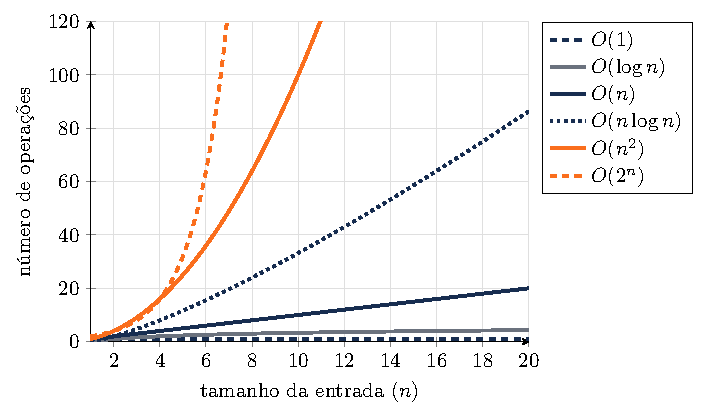
\includegraphics[width=\linewidth,keepaspectratio]{imagens/capitulo-02_crescimento.pdf}
\end{center}

Para sentir a diferença na prática, imagine um computador que faz \textbf{1 milhão de operações por segundo}. Quanto tempo cada classe levaria?

\begin{center}
\begin{tabular}{@{}p{0.2\linewidth}p{0.3\linewidth}p{0.36\linewidth}@{}}
\toprule
\rowcolor{headergray}
\tblheader{Classe} & \tblheader{$n = 1.000$} & \tblheader{$n = 1.000.000$} \\
\midrule
$O(\log n)$ & 10 microssegundos & 20 microssegundos \\
\rowcolor{rowgray} $O(n)$ & 1 milissegundo & 1 segundo \\
$O(n \log n)$ & 10 milissegundos & 20 segundos \\
\rowcolor{rowgray} $O(n^2)$ & 1 segundo & cerca de 11,6 dias \\
$O(2^n)$ & mais que a idade do universo & impossível \\
\bottomrule
\end{tabular}
\end{center}

A tabela explica por que a escolha do algoritmo importa mais que a velocidade do computador. Um processador mil vezes mais rápido transforma os 11,6 dias do $O(n^2)$ em cerca de 17 minutos, mas um algoritmo $O(n \log n)$, na máquina antiga, resolve o mesmo problema em 20 segundos.

\subsection{2.7 Analisando código passo a passo}

Com as regras da seção 2.5, dá para descobrir a complexidade lendo o código. Veja os padrões mais comuns.

\subsubsection{Laço simples: O(n)}

\begin{codigo}
\begin{Verbatim}[breaklines=true, breaksymbolleft={}, fontsize=\footnotesize]
// encontra o maior valor do vetor: percorre cada elemento uma vez
int maiorValor(int v[], int n) {
    int maior = v[0];
    for (int i = 1; i < n; i++) {
        if (v[i] > maior) {
            maior = v[i];
        }
    }
    return maior;
}
\end{Verbatim}
\end{codigo}

\subsubsection{Laços aninhados: O(n²)}

\begin{codigo}
\begin{Verbatim}[breaklines=true, breaksymbolleft={}, fontsize=\footnotesize]
// verifica se o vetor tem algum valor repetido, comparando todos os pares
bool temRepetido(int v[], int n) {
    for (int i = 0; i < n; i++) {
        for (int j = i + 1; j < n; j++) {
            if (v[i] == v[j]) {
                return true;
            }
        }
    }
    return false;
}
\end{Verbatim}
\end{codigo}

O laço interno começa em \texttt{i + 1}, então ele dá $n-1$ voltas, depois $n-2$, e assim por diante. A soma é $n(n-1)/2$ comparações no pior caso. Descartando a constante $1/2$ e o termo menor, a função é $O(n^2)$.

\subsubsection{Laço que divide a entrada: O(log n)}

\begin{codigo}
\begin{Verbatim}[breaklines=true, breaksymbolleft={}, fontsize=\footnotesize]
// quantas vezes n pode ser dividido por 2 até chegar a 1?
int contarDivisoes(int n) {
    int passos = 0;
    while (n > 1) {
        n = n / 2;
        passos++;
    }
    return passos;
}

int main() {
    cout << contarDivisoes(1000) << endl;     // 9
    cout << contarDivisoes(1000000) << endl;  // 19
}
\end{Verbatim}
\end{codigo}

Sempre que um algoritmo \textbf{descarta metade} do problema a cada passo, ele é logarítmico. Multiplicar a entrada por mil acrescenta só uns 10 passos. É o segredo da busca binária (Capítulo 7) e das árvores balanceadas (Capítulo 5).

\subsubsection{Laço que divide dentro de um laço linear: O(n log n)}

\begin{codigo}
\begin{Verbatim}[breaklines=true, breaksymbolleft={}, fontsize=\footnotesize]
int exemploNLogN(int n) {
    int total = 0;
    for (int i = 0; i < n; i++) {           // n vezes
        for (int j = n; j > 1; j = j / 2) { // log n vezes
            total++;
        }
    }
    return total;
}
\end{Verbatim}
\end{codigo}

Esse é o padrão dos bons algoritmos de ordenação, como o merge sort (Capítulo 8): cada um dos $\log n$ níveis de divisão faz um trabalho linear.

\subsubsection{Recursão}

Em Algoritmos I você viu que uma função recursiva chama a si mesma. Para analisá-la, conte quantas chamadas acontecem e quanto trabalho cada uma faz.

\begin{codigo}
\begin{Verbatim}[breaklines=true, breaksymbolleft={}, fontsize=\footnotesize]
// fatorial: n chamadas, cada uma com trabalho constante -> O(n)
long long fatorial(int n) {
    if (n <= 1) return 1;
    return n * fatorial(n - 1);
}

// Fibonacci recursivo: cada chamada gera outras duas -> O(2^n)
long long fibRecursivo(int n) {
    if (n <= 1) return n;
    return fibRecursivo(n - 1) + fibRecursivo(n - 2);
}

// Fibonacci com laço: guarda só os dois últimos valores -> O(n)
long long fibIterativo(int n) {
    long long anterior = 0, atual = 1;
    for (int i = 0; i < n; i++) {
        long long proximo = anterior + atual;
        anterior = atual;
        atual = proximo;
    }
    return anterior;
}

int main() {
    cout << fatorial(10) << endl;      // 3628800
    cout << fibRecursivo(30) << endl;  // 832040, após mais de 1 milhão de chamadas
    cout << fibIterativo(30) << endl;  // 832040, com apenas 30 voltas
}
\end{Verbatim}
\end{codigo}

O Fibonacci recursivo é um ótimo alerta: o código é curto e elegante, mas recalcula os mesmos valores muitas vezes. Para \texttt{fibRecursivo(50)}, seriam bilhões de chamadas. A versão com laço resolve em 50 passos. No Capítulo 9 você vai ver a programação dinâmica, uma técnica que conserta exatamente esse tipo de desperdício.

\begin{destaque}{Comparando com Python}
Em Python, operações que parecem instantâneas podem esconder um laço inteiro. Saber a complexidade delas evita surpresas:

\begin{codigo}
\begin{Verbatim}[breaklines=true, breaksymbolleft={}, fontsize=\footnotesize]
nomes = ["ana", "bia", "caio", "davi"]

print("davi" in nomes)   # O(n): percorre a lista até achar
nomes.append("eva")      # O(1) em média: coloca no fim
nomes.insert(0, "zoe")   # O(n): desloca todos os elementos
nomes.pop()              # O(1): remove do fim
nomes.pop(0)             # O(n): desloca todos os elementos

conjunto = set(nomes)
print("davi" in conjunto)  # O(1) em média: usa tabela hash
\end{Verbatim}
\end{codigo}

Uma linha como \texttt{if x in lista} dentro de um laço transforma um algoritmo que parecia $O(n)$ em $O(n^2)$. Em C++, como você escreve os laços, esse custo fica visível no próprio código.
\end{destaque}

\subsection{2.8 Complexidade de espaço}

A mesma notação mede a \textbf{memória extra} que o algoritmo usa, além da própria entrada.

\begin{itemize}
  \item \texttt{somarVetor} e \texttt{fibIterativo} usam só algumas variáveis, não importa o tamanho de $n$: espaço $O(1)$.
  \item Um algoritmo que cria uma cópia do vetor para trabalhar nela usa espaço $O(n)$.
  \item O \texttt{fatorial} recursivo também usa espaço $O(n)$, mesmo sem criar vetores: cada chamada que ainda não terminou ocupa um espaço na pilha de execução, e há $n$ chamadas abertas ao mesmo tempo.
\end{itemize}

Muitas vezes é possível trocar espaço por tempo: guardar resultados já calculados gasta memória, mas evita refazer contas. Essa troca é a base da programação dinâmica.

\begin{destaque}{Para saber mais: Ômega e Theta}
Além do Big O, existem outras duas notações. A notação $\Omega$ (ômega) indica um \textbf{limite inferior}: o algoritmo faz \textit{pelo menos} aquela quantidade de trabalho. A notação $\Theta$ (theta) indica um \textbf{limite exato}: o crescimento é \textit{exatamente} daquela ordem, nem mais nem menos. Na prática, quando alguém diz ``a busca sequencial é $O(n)$'', costuma querer dizer que o pior caso cresce exatamente como $n$. Nesta apostila, seguindo o uso comum, usaremos o Big O.
\end{destaque}

\subsection{Erros Comuns}

\begin{itemize}
  \item \textbf{Confundir Big O com tempo em segundos.} $O(n)$ não diz quanto tempo o programa leva, e sim como esse tempo cresce. Um algoritmo $O(n)$ pode ser mais lento que um $O(n^2)$ para entradas pequenas.
  \item \textbf{Manter constantes e termos menores.} Escrever $O(2n + 10)$ está tecnicamente certo, mas o correto é simplificar para $O(n)$.
  \item \textbf{Somar quando deveria multiplicar.} Dois laços de $n$ voltas \textit{um depois do outro} dão $O(n)$; \textit{um dentro do outro} dão $O(n^2)$.
  \item \textbf{Esquecer o custo das operações de biblioteca.} Chamar uma função que percorre a estrutura inteira (como \texttt{in} em uma lista do Python) dentro de um laço multiplica a complexidade.
  \item \textbf{Analisar só o melhor caso.} Dizer que a busca sequencial é $O(1)$ porque às vezes o valor está na primeira posição esconde o comportamento real. Use o pior caso como referência.
  \item \textbf{Ignorar o espaço da recursão.} Uma função recursiva com $n$ chamadas abertas ao mesmo tempo usa memória $O(n)$, e com $n$ muito grande pode estourar a pilha de execução.
\end{itemize}

\newpage
\section{Capítulo 3 -- Listas Encadeadas}

Em Algoritmos I você trabalhou com vetores: uma sequência de posições lado a lado na memória, com tamanho definido na criação. Neste capítulo você vai construir uma estrutura que cresce e encolhe conforme a necessidade, sem desperdiçar espaço e sem deslocar elementos: a \textbf{lista encadeada}. Ela é a primeira estrutura dinâmica do livro e a base de várias outras, como pilhas, filas e grafos.

\subsection{3.1 Quando o vetor não basta}

Imagine um sistema que registra os pedidos de uma loja ao longo do dia. Não dá para saber quantos pedidos vão chegar. Se você criar um vetor de 1.000 posições e chegarem 30 pedidos, desperdiçou memória; se chegarem 1.500, faltou espaço. O vetor dinâmico do Capítulo 1 resolve parte do problema, mas cada vez que enche precisa copiar tudo para um espaço maior.

Há um segundo problema: inserir ou remover \textbf{no meio}. Para colocar um pedido urgente na frente da fila de um vetor, todos os outros precisam andar uma posição. Com 1 milhão de pedidos, isso é 1 milhão de movimentações.

A lista encadeada resolve as duas questões com uma ideia simples: cada elemento fica em um \textbf{nó} criado separadamente na memória, e cada nó guarda, além do valor, um \textbf{ponteiro para o próximo}. Os nós podem estar em qualquer lugar da memória; o que os mantém em ordem são os ponteiros.

\begin{center}
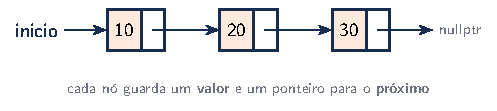
\includegraphics[width=0.9\linewidth,keepaspectratio]{imagens/capitulo-03_lista.pdf}
\end{center}

A lista só precisa guardar onde está o primeiro nó (\texttt{inicio}). A partir dele, seguindo os ponteiros, chega-se a todos os outros. O último nó aponta para \texttt{nullptr}, que marca o fim.

\subsection{3.2 Tipo Abstrato de Dados}

Antes de programar, vale separar duas perguntas: \textit{o que} a lista faz e \textit{como} ela faz. A resposta à primeira pergunta é a \textbf{interface}: o conjunto de operações que quem usa a lista pode chamar. Um \textbf{Tipo Abstrato de Dados} (TAD) é justamente isso: um tipo definido pelas operações que oferece, sem expor como elas são implementadas.

\begin{center}
\begin{tabular}{@{}p{0.34\linewidth}p{0.52\linewidth}@{}}
\toprule
\rowcolor{headergray}
\tblheader{Operação} & \tblheader{O que faz} \\
\midrule
\texttt{inserirInicio(v)} & coloca o valor \texttt{v} no começo \\
\rowcolor{rowgray} \texttt{inserirFim(v)} & coloca o valor \texttt{v} no final \\
\texttt{inserirNaPosicao(p, v)} & coloca \texttt{v} na posição \texttt{p} \\
\rowcolor{rowgray} \texttt{remover(v)} & retira a primeira ocorrência de \texttt{v} \\
\texttt{contem(v)} & diz se \texttt{v} está na lista \\
\rowcolor{rowgray} \texttt{quantidade()} & quantos elementos a lista tem \\
\texttt{vazia()} & diz se a lista está vazia \\
\bottomrule
\end{tabular}
\end{center}

A mesma interface poderia ser implementada com um vetor ou com nós encadeados. Quem usa a lista não precisa saber qual das duas foi escolhida: chama as mesmas operações e recebe os mesmos resultados. O que muda é o \textbf{custo} de cada operação, e é por isso que estudamos as implementações.

\subsection{3.3 O nó e a classe ListaEncadeada}

O nó é uma struct com o valor e o ponteiro para o próximo, como você viu no Capítulo 1. A lista é uma classe que guarda o ponteiro para o primeiro nó, um ponteiro para o último (veremos por quê) e a quantidade de elementos:

\begin{codigo}
\begin{Verbatim}[breaklines=true, breaksymbolleft={}, fontsize=\footnotesize]
// trecho: o nó e os dados da classe ListaEncadeada
struct No {
    int valor;
    No *proximo;
};

class ListaEncadeada {
private:
    No *inicio;    // primeiro nó (nullptr se a lista estiver vazia)
    No *fim;       // último nó
    int tamanho;   // quantidade de elementos
    // ... operações (a seguir)
};
\end{Verbatim}
\end{codigo}

Uma lista recém-criada não tem nós: \texttt{inicio} e \texttt{fim} valem \texttt{nullptr} e o tamanho é zero. Esse estado é a \textbf{lista vazia}, e toda operação precisa tratá-lo com cuidado.

\subsection{3.4 Inserindo elementos}

\subsubsection{No início: O(1)}

Inserir no início exige só dois passos, não importa quantos elementos a lista tenha: o novo nó aponta para o atual primeiro, e \texttt{inicio} passa a apontar para o novo nó.

\begin{center}
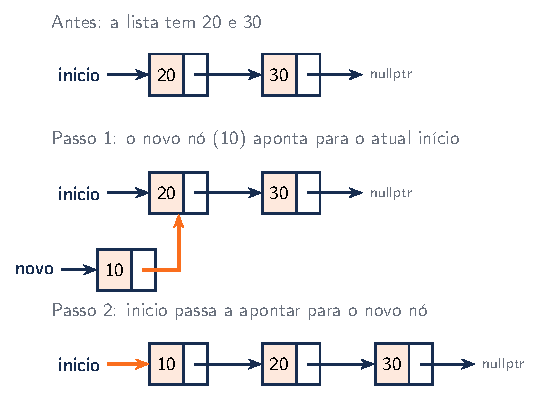
\includegraphics[width=0.95\linewidth,keepaspectratio]{imagens/capitulo-03_inserir_inicio.pdf}
\end{center}

\begin{codigo}
\begin{Verbatim}[breaklines=true, breaksymbolleft={}, fontsize=\footnotesize]
// trecho da classe ListaEncadeada
void inserirInicio(int valor) {
    No *novo = new No{valor, inicio};  // passo 1: aponta para o atual início
    inicio = novo;                     // passo 2: início passa a ser o novo nó
    if (fim == nullptr) {              // a lista estava vazia:
        fim = novo;                    // o novo nó também é o último
    }
    tamanho++;
}
\end{Verbatim}
\end{codigo}

A ordem dos passos importa. Se você fizer primeiro \texttt{inicio = novo}, perde a referência para o antigo primeiro nó, e o resto da lista fica inacessível.

\subsubsection{No fim: O(1) graças ao ponteiro fim}

Sem o ponteiro \texttt{fim}, inserir no final exigiria percorrer a lista inteira até achar o último nó: $O(n)$. Guardando um ponteiro para o último, basta ligá-lo ao novo nó:

\begin{codigo}
\begin{Verbatim}[breaklines=true, breaksymbolleft={}, fontsize=\footnotesize]
// trecho da classe ListaEncadeada
void inserirFim(int valor) {
    No *novo = new No{valor, nullptr};
    if (fim == nullptr) {        // lista vazia: o novo nó é o primeiro e o último
        inicio = novo;
        fim = novo;
    } else {
        fim->proximo = novo;     // o antigo último aponta para o novo
        fim = novo;              // e o novo passa a ser o último
    }
    tamanho++;
}
\end{Verbatim}
\end{codigo}

Esse é um exemplo de troca entre espaço e tempo: um ponteiro a mais na classe transforma uma operação $O(n)$ em $O(1)$.

\subsubsection{Em uma posição qualquer: O(n)}

Para inserir na posição \texttt{p}, é preciso caminhar até o nó da posição \texttt{p - 1} e ligar o novo nó depois dele. A caminhada custa $O(n)$; a ligação em si, $O(1)$.

\begin{codigo}
\begin{Verbatim}[breaklines=true, breaksymbolleft={}, fontsize=\footnotesize]
// trecho da classe ListaEncadeada
bool inserirNaPosicao(int pos, int valor) {
    if (pos < 0 || pos > tamanho) return false;          // posição inválida
    if (pos == 0) { inserirInicio(valor); return true; }
    if (pos == tamanho) { inserirFim(valor); return true; }

    No *anterior = inicio;
    for (int i = 0; i < pos - 1; i++) {                  // caminha até pos - 1
        anterior = anterior->proximo;
    }
    anterior->proximo = new No{valor, anterior->proximo};
    tamanho++;
    return true;
}
\end{Verbatim}
\end{codigo}

\subsection{3.5 Percorrendo e buscando}

Percorrer a lista é sempre o mesmo movimento: começar em \texttt{inicio} e seguir \texttt{proximo} até chegar em \texttt{nullptr}. Buscar um valor é percorrer comparando, e por isso custa $O(n)$ no pior caso, como a busca sequencial do Capítulo 2.

\begin{codigo}
\begin{Verbatim}[breaklines=true, breaksymbolleft={}, fontsize=\footnotesize]
// trecho da classe ListaEncadeada
bool contem(int valor) const {
    for (No *atual = inicio; atual != nullptr; atual = atual->proximo) {
        if (atual->valor == valor) {
            return true;
        }
    }
    return false;
}
\end{Verbatim}
\end{codigo}

Repare que não existe atalho para chegar ao quinto elemento: é preciso passar pelos quatro anteriores. Acessar uma posição por índice, que no vetor é $O(1)$, na lista encadeada é $O(n)$. Essa é a principal desvantagem da lista.

\subsection{3.6 Removendo elementos}

Para remover um nó, o nó \textbf{anterior} a ele passa a apontar para o \textbf{seguinte}. O nó removido fica fora da corrente e pode ser liberado com \texttt{delete}.

\begin{center}
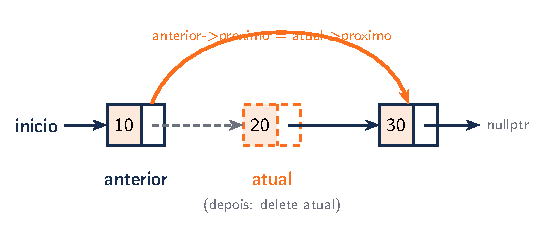
\includegraphics[width=0.9\linewidth,keepaspectratio]{imagens/capitulo-03_remover.pdf}
\end{center}

Como cada nó só conhece o próximo, a busca precisa andar com \textbf{dois ponteiros}: \texttt{atual}, que procura o valor, e \texttt{anterior}, que fica um passo atrás. A remoção ainda precisa tratar casos especiais: lista vazia, valor ausente, remoção do primeiro nó e remoção do último.

\begin{codigo}
\begin{Verbatim}[breaklines=true, breaksymbolleft={}, fontsize=\footnotesize]
// trecho da classe ListaEncadeada
bool remover(int valor) {
    No *anterior = nullptr;
    No *atual = inicio;
    while (atual != nullptr && atual->valor != valor) {
        anterior = atual;
        atual = atual->proximo;
    }
    if (atual == nullptr) {              // não encontrou (ou lista vazia)
        return false;
    }
    if (anterior == nullptr) {           // era o primeiro nó
        inicio = atual->proximo;
    } else {                             // estava no meio ou no fim
        anterior->proximo = atual->proximo;
    }
    if (atual == fim) {                  // era o último nó
        fim = anterior;
    }
    delete atual;
    tamanho--;
    return true;
}
\end{Verbatim}
\end{codigo}

\subsection{3.7 O programa completo}

Juntando as operações, a classe fica assim. Repare no destrutor, que percorre a lista liberando cada nó, e nas duas linhas com \texttt{= delete}, explicadas logo depois do código.

\begin{codigo}
\begin{Verbatim}[breaklines=true, breaksymbolleft={}, fontsize=\footnotesize]
struct No {
    int valor;
    No *proximo;
};

class ListaEncadeada {
private:
    No *inicio;
    No *fim;
    int tamanho;

public:
    ListaEncadeada() : inicio(nullptr), fim(nullptr), tamanho(0) {}

    // libera todos os nós quando a lista deixa de existir
    ~ListaEncadeada() {
        No *atual = inicio;
        while (atual != nullptr) {
            No *seguinte = atual->proximo;  // guarda antes de apagar
            delete atual;
            atual = seguinte;
        }
    }

    // impede cópias: duas listas não podem dividir os mesmos nós
    ListaEncadeada(const ListaEncadeada &) = delete;
    ListaEncadeada &operator=(const ListaEncadeada &) = delete;

    bool vazia() const { return tamanho == 0; }
    int quantidade() const { return tamanho; }

    void inserirInicio(int valor) {
        No *novo = new No{valor, inicio};
        inicio = novo;
        if (fim == nullptr) {
            fim = novo;
        }
        tamanho++;
    }

    void inserirFim(int valor) {
        No *novo = new No{valor, nullptr};
        if (fim == nullptr) {
            inicio = novo;
            fim = novo;
        } else {
            fim->proximo = novo;
            fim = novo;
        }
        tamanho++;
    }

    bool inserirNaPosicao(int pos, int valor) {
        if (pos < 0 || pos > tamanho) return false;
        if (pos == 0) { inserirInicio(valor); return true; }
        if (pos == tamanho) { inserirFim(valor); return true; }
        No *anterior = inicio;
        for (int i = 0; i < pos - 1; i++) {
            anterior = anterior->proximo;
        }
        anterior->proximo = new No{valor, anterior->proximo};
        tamanho++;
        return true;
    }

    bool contem(int valor) const {
        for (No *atual = inicio; atual != nullptr; atual = atual->proximo) {
            if (atual->valor == valor) {
                return true;
            }
        }
        return false;
    }

    bool remover(int valor) {
        No *anterior = nullptr;
        No *atual = inicio;
        while (atual != nullptr && atual->valor != valor) {
            anterior = atual;
            atual = atual->proximo;
        }
        if (atual == nullptr) {
            return false;
        }
        if (anterior == nullptr) {
            inicio = atual->proximo;
        } else {
            anterior->proximo = atual->proximo;
        }
        if (atual == fim) {
            fim = anterior;
        }
        delete atual;
        tamanho--;
        return true;
    }

    void imprimir() const {
        cout << "[ ";
        for (No *atual = inicio; atual != nullptr; atual = atual->proximo) {
            cout << atual->valor << " ";
        }
        cout << "]" << endl;
    }
};

int main() {
    ListaEncadeada lista;
    lista.inserirFim(20);
    lista.inserirFim(30);
    lista.inserirInicio(10);
    lista.imprimir();                      // [ 10 20 30 ]

    lista.inserirNaPosicao(2, 25);
    lista.imprimir();                      // [ 10 20 25 30 ]

    cout << boolalpha << lista.contem(25) << endl;   // true

    lista.remover(10);                     // remove o primeiro
    lista.remover(30);                     // remove o último
    lista.remover(99);                     // não existe: nada acontece
    lista.imprimir();                      // [ 20 25 ]
    cout << lista.quantidade() << endl;    // 2
}
\end{Verbatim}
\end{codigo}

\begin{destaque}{Por que proibir cópias?}
Sem as linhas com \texttt{= delete}, o C++ permitiria escrever \texttt{ListaEncadeada outra = lista;}. A cópia automática copiaria só os ponteiros, e as duas listas passariam a apontar para os \textbf{mesmos nós}. Quando a primeira deixasse de existir, o destrutor liberaria os nós; quando a segunda deixasse de existir, tentaria liberá-los de novo, e o programa travaria. Proibir a cópia é a forma mais simples de evitar o problema. Uma classe que precisa ser copiável deve implementar a cópia nó por nó.
\end{destaque}

\subsection{3.8 Lista duplamente encadeada}

Na lista simples, cada nó só conhece o próximo. Isso tem duas consequências incômodas: não dá para percorrer a lista de trás para frente, e remover o último nó custa $O(n)$, porque é preciso encontrar o penúltimo caminhando desde o início.

A \textbf{lista duplamente encadeada} acrescenta em cada nó um ponteiro para o \textbf{anterior}:

\begin{center}
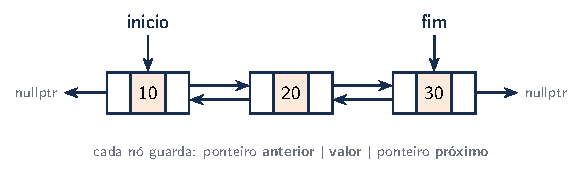
\includegraphics[width=0.95\linewidth,keepaspectratio]{imagens/capitulo-03_dupla.pdf}
\end{center}

Com os dois ponteiros, inserir e remover nas duas pontas custa $O(1)$, e a lista pode ser percorrida nos dois sentidos. O preço é um ponteiro a mais por nó e mais cuidado: cada operação precisa manter \texttt{anterior} e \texttt{proximo} coerentes.

\begin{codigo}
\begin{Verbatim}[breaklines=true, breaksymbolleft={}, fontsize=\footnotesize]
struct NoDuplo {
    int valor;
    NoDuplo *anterior;
    NoDuplo *proximo;
};

class ListaDupla {
private:
    NoDuplo *inicio;
    NoDuplo *fim;
    int tamanho;

public:
    ListaDupla() : inicio(nullptr), fim(nullptr), tamanho(0) {}

    ~ListaDupla() {
        while (!vazia()) {
            removerInicio();
        }
    }

    ListaDupla(const ListaDupla &) = delete;
    ListaDupla &operator=(const ListaDupla &) = delete;

    bool vazia() const { return tamanho == 0; }

    void inserirInicio(int valor) {
        NoDuplo *novo = new NoDuplo{valor, nullptr, inicio};
        if (inicio == nullptr) {
            fim = novo;
        } else {
            inicio->anterior = novo;
        }
        inicio = novo;
        tamanho++;
    }

    void inserirFim(int valor) {
        NoDuplo *novo = new NoDuplo{valor, fim, nullptr};
        if (fim == nullptr) {
            inicio = novo;
        } else {
            fim->proximo = novo;
        }
        fim = novo;
        tamanho++;
    }

    // as duas remoções são O(1): não é preciso procurar o vizinho
    bool removerInicio() {
        if (vazia()) return false;
        NoDuplo *velho = inicio;
        inicio = inicio->proximo;
        if (inicio == nullptr) {
            fim = nullptr;           // a lista ficou vazia
        } else {
            inicio->anterior = nullptr;
        }
        delete velho;
        tamanho--;
        return true;
    }

    bool removerFim() {
        if (vazia()) return false;
        NoDuplo *velho = fim;
        fim = fim->anterior;         // o penúltimo, sem precisar procurar
        if (fim == nullptr) {
            inicio = nullptr;
        } else {
            fim->proximo = nullptr;
        }
        delete velho;
        tamanho--;
        return true;
    }

    void imprimir() const {
        for (NoDuplo *a = inicio; a != nullptr; a = a->proximo) cout << a->valor << " ";
        cout << endl;
    }

    void imprimirInvertido() const {
        for (NoDuplo *a = fim; a != nullptr; a = a->anterior) cout << a->valor << " ";
        cout << endl;
    }
};

int main() {
    ListaDupla lista;
    lista.inserirFim(20);
    lista.inserirFim(30);
    lista.inserirInicio(10);
    lista.imprimir();            // 10 20 30
    lista.imprimirInvertido();   // 30 20 10
    lista.removerFim();
    lista.removerInicio();
    lista.imprimir();            // 20
}
\end{Verbatim}
\end{codigo}

\subsection{3.9 Lista circular}

Em uma \textbf{lista circular}, o último nó não aponta para \texttt{nullptr}: aponta de volta para o primeiro. A lista vira um anel, sem começo nem fim naturais.

\begin{center}
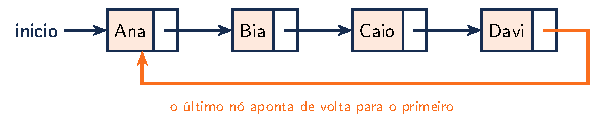
\includegraphics[width=0.95\linewidth,keepaspectratio]{imagens/capitulo-03_circular.pdf}
\end{center}

Ela é útil sempre que os elementos são atendidos em rodízio, voltando ao primeiro depois do último: turnos de um jogo, a fila de processos que dividem o processador, as músicas de uma playlist em repetição.

Um detalhe elegante: basta guardar um ponteiro para o \textbf{último} nó. O primeiro é sempre \texttt{ultimo->proximo}, então as duas pontas ficam acessíveis em $O(1)$ com um único ponteiro.

\begin{codigo}
\begin{Verbatim}[breaklines=true, breaksymbolleft={}, fontsize=\footnotesize]
struct Jogador {
    string nome;
    Jogador *proximo;
};

class Rodizio {
private:
    Jogador *ultimo = nullptr;   // ultimo->proximo é o primeiro

public:
    ~Rodizio() {
        if (ultimo == nullptr) return;
        Jogador *atual = ultimo->proximo;
        ultimo->proximo = nullptr;          // abre o anel para poder parar
        while (atual != nullptr) {
            Jogador *seguinte = atual->proximo;
            delete atual;
            atual = seguinte;
        }
    }

    Rodizio() = default;
    Rodizio(const Rodizio &) = delete;
    Rodizio &operator=(const Rodizio &) = delete;

    void adicionar(const string &nome) {
        Jogador *novo = new Jogador{nome, nullptr};
        if (ultimo == nullptr) {
            novo->proximo = novo;           // um só jogador: aponta para si mesmo
        } else {
            novo->proximo = ultimo->proximo; // o novo aponta para o primeiro
            ultimo->proximo = novo;          // o antigo último aponta para o novo
        }
        ultimo = novo;                       // o novo passa a ser o último
    }

    void jogar(int turnos) const {
        if (ultimo == nullptr) return;
        Jogador *vez = ultimo->proximo;      // começa pelo primeiro
        for (int t = 1; t <= turnos; t++) {
            cout << "Turno " << t << ": " << vez->nome << endl;
            vez = vez->proximo;              // depois do último, volta ao primeiro
        }
    }
};

int main() {
    Rodizio jogo;
    jogo.adicionar("Ana");
    jogo.adicionar("Bia");
    jogo.adicionar("Caio");
    jogo.jogar(5);   // Ana, Bia, Caio, Ana, Bia
}
\end{Verbatim}
\end{codigo}

Cuidado com a parada: em uma lista circular, percorrer até encontrar \texttt{nullptr} gera um laço infinito. Por isso o percurso para por contagem (como em \texttt{jogar}) ou ao voltar ao nó de partida, e o destrutor ``abre'' o anel antes de liberar os nós.

\subsection{3.10 Vetor ou lista encadeada?}

Nenhuma das duas estruturas é melhor em tudo. A escolha depende de quais operações o seu problema faz com mais frequência:

\begin{center}
\begin{tabular}{@{}p{0.34\linewidth}p{0.16\linewidth}p{0.18\linewidth}p{0.16\linewidth}@{}}
\toprule
\rowcolor{headergray}
\tblheader{Operação} & \tblheader{Vetor} & \tblheader{Lista simples} & \tblheader{Lista dupla} \\
\midrule
Acessar a posição $i$ & $O(1)$ & $O(n)$ & $O(n)$ \\
\rowcolor{rowgray} Inserir no início & $O(n)$ & $O(1)$ & $O(1)$ \\
Inserir no fim & $O(1)$* & $O(1)$ & $O(1)$ \\
\rowcolor{rowgray} Remover do início & $O(n)$ & $O(1)$ & $O(1)$ \\
Remover do fim & $O(1)$ & $O(n)$ & $O(1)$ \\
\rowcolor{rowgray} Buscar um valor & $O(n)$ & $O(n)$ & $O(n)$ \\
Memória extra por elemento & nenhuma & 1 ponteiro & 2 ponteiros \\
\bottomrule
\end{tabular}
\end{center}

{\footnotesize * No vetor dinâmico, quase sempre $O(1)$; de vez em quando, quando enche, a cópia para um espaço maior custa $O(n)$. Na média, continua $O(1)$: dizemos que é $O(1)$ \textbf{amortizado}.}

Em resumo: prefira o \textbf{vetor} quando o acesso por posição for frequente e as inserções acontecerem no fim; prefira a \textbf{lista} quando houver muitas inserções e remoções nas pontas ou no meio de uma sequência que você já está percorrendo. Na prática, vetores também se beneficiam de estarem contínuos na memória, o que o processador aproveita muito bem; por isso, para listas pequenas, o vetor costuma ser mais rápido mesmo quando a tabela sugere o contrário.

\begin{destaque}{Comparando com Python}
A \texttt{list} do Python é um vetor dinâmico, não uma lista encadeada: acessar \texttt{lista[i]} é $O(1)$, mas \texttt{lista.insert(0, x)} é $O(n)$. Quando você precisa inserir e remover nas duas pontas, a escolha certa é o \texttt{deque}, do módulo \texttt{collections}, implementado com blocos encadeados. E, se quiser, dá para escrever uma lista encadeada em Python com a mesma ideia de nós:

\begin{codigo}
\begin{Verbatim}[breaklines=true, breaksymbolleft={}, fontsize=\footnotesize]
from collections import deque

class No:
    def __init__(self, valor, proximo=None):
        self.valor = valor
        self.proximo = proximo     # referência para o próximo nó (ou None)

inicio = No(10, No(20, No(30)))   # 10 -> 20 -> 30
atual = inicio
while atual is not None:
    print(atual.valor, end=" ")
    atual = atual.proximo
print()

pedidos = deque([20, 30])
pedidos.appendleft(10)           # O(1), como inserirInicio
pedidos.append(40)               # O(1), como inserirFim
print(pedidos.popleft())         # 10, O(1)
\end{Verbatim}
\end{codigo}

Em Python não há \texttt{delete}: quando nenhum nó aponta mais para um objeto, a coleta de lixo o remove.
\end{destaque}

A biblioteca padrão do C++ também oferece listas prontas: \texttt{std::forward\_list} (simplesmente encadeada) e \texttt{std::list} (duplamente encadeada). Agora que você sabe como funcionam por dentro, use-as nos seus projetos.

\subsection{Erros Comuns}

\begin{itemize}
  \item \textbf{Perder o resto da lista.} Ao inserir no início, atualizar \texttt{inicio} antes de ligar o novo nó ao antigo primeiro deixa todos os outros nós inacessíveis.
  \item \textbf{Esquecer a lista vazia.} Toda operação precisa funcionar quando \texttt{inicio} é \texttt{nullptr}. Acessar \texttt{inicio->valor} em uma lista vazia derruba o programa.
  \item \textbf{Não atualizar o ponteiro \texttt{fim}.} Ao remover o último nó, \texttt{fim} precisa passar a apontar para o anterior (ou para \texttt{nullptr}, se a lista ficou vazia).
  \item \textbf{Usar o nó depois do \texttt{delete}.} No destrutor, guarde o \texttt{proximo} em uma variável \textit{antes} de liberar o nó atual.
  \item \textbf{Esquecer o destrutor.} Sem ele, todos os nós ficam presos na memória quando a lista deixa de existir.
  \item \textbf{Copiar uma lista sem tratar a cópia.} A cópia automática divide os mesmos nós entre duas listas e causa \texttt{delete} duplo. Proíba a cópia ou implemente-a nó por nó.
  \item \textbf{Esquecer um dos ponteiros na lista dupla.} Cada inserção e remoção precisa atualizar \texttt{anterior} e \texttt{proximo} dos vizinhos.
  \item \textbf{Laço infinito na lista circular.} Na lista circular, nenhum nó aponta para \texttt{nullptr}: o percurso precisa parar por contagem ou ao voltar ao início.
\end{itemize}

\newpage
\section{Capítulo 4 -- Pilhas e Filas}

A lista encadeada do Capítulo 3 permite inserir e remover em qualquer ponto. Muitos problemas, porém, precisam do contrário: de uma estrutura que \textbf{restringe} onde se pode inserir e remover. Essas restrições não são uma limitação, e sim uma garantia de ordem. Neste capítulo você vai construir as duas estruturas restritas mais usadas da computação: a \textbf{pilha} e a \textbf{fila}. Ambas serão genéricas, com templates (Capítulo 1), e construídas com nós encadeados (Capítulo 3).

\subsection{4.1 Estruturas com regras de acesso}

Pense em uma pilha de pratos: você coloca um prato sempre em cima e, quando precisa de um, pega o de cima. O último prato colocado é o primeiro a ser usado. Agora pense na fila de um banco: quem chega vai para o final, e quem é atendido sai pela frente. O primeiro a chegar é o primeiro a sair.

Essas duas regras têm nomes:

\begin{itemize}
  \item \textbf{LIFO} (\textit{Last In, First Out}, o último a entrar é o primeiro a sair): é a regra da \textbf{pilha}.
  \item \textbf{FIFO} (\textit{First In, First Out}, o primeiro a entrar é o primeiro a sair): é a regra da \textbf{fila}.
\end{itemize}

Você usa as duas o tempo todo, mesmo sem perceber. O botão de desfazer (Ctrl+Z) de um editor é uma pilha: desfaz primeiro a última ação. Os documentos enviados para uma impressora formam uma fila: são impressos na ordem em que chegaram.

\subsection{4.2 A pilha}

Em uma pilha, todas as operações acontecem em uma única ponta, chamada \textbf{topo}.

\begin{center}
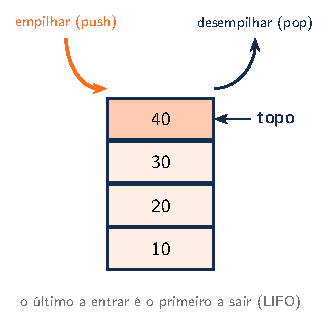
\includegraphics[width=0.6\linewidth,keepaspectratio]{imagens/capitulo-04_pilha.pdf}
\end{center}

\begin{center}
\begin{tabular}{@{}p{0.3\linewidth}p{0.42\linewidth}p{0.14\linewidth}@{}}
\toprule
\rowcolor{headergray}
\tblheader{Operação} & \tblheader{O que faz} & \tblheader{Custo} \\
\midrule
\texttt{empilhar(v)} & coloca \texttt{v} no topo (\textit{push}) & $O(1)$ \\
\rowcolor{rowgray} \texttt{desempilhar()} & retira e devolve o topo (\textit{pop}) & $O(1)$ \\
\texttt{espiar()} & devolve o topo sem retirar (\textit{top}) & $O(1)$ \\
\rowcolor{rowgray} \texttt{vazia()} & diz se não há elementos & $O(1)$ \\
\texttt{quantidade()} & quantos elementos há & $O(1)$ \\
\bottomrule
\end{tabular}
\end{center}

\subsection{4.3 Pilha com nós encadeados}

Na lista encadeada, inserir e remover no \textbf{início} custa $O(1)$. Então basta usar o início da lista como topo da pilha: empilhar é inserir no início, desempilhar é remover do início. Cada nó aponta para o que está \textbf{abaixo} dele.

Repare em duas novidades. O nó agora fica \textbf{dentro} da classe, porque só a pilha precisa conhecê-lo. E desempilhar uma pilha vazia é um erro de quem chama: em vez de devolver um valor inventado, a função \textbf{lança uma exceção} com \texttt{throw}, que interrompe a operação e pode ser tratada com \texttt{try}/\texttt{catch}.

\begin{codigo}
\begin{Verbatim}[breaklines=true, breaksymbolleft={}, fontsize=\footnotesize]
#include <stdexcept>   // runtime_error

template <typename T>
class Pilha {
private:
    struct No {
        T valor;
        No *abaixo;    // o nó que está embaixo deste
    };
    No *topo = nullptr;
    int tamanho = 0;

public:
    Pilha() = default;
    ~Pilha() {
        while (!vazia()) {
            desempilhar();
        }
    }
    Pilha(const Pilha &) = delete;
    Pilha &operator=(const Pilha &) = delete;

    bool vazia() const { return topo == nullptr; }
    int quantidade() const { return tamanho; }

    void empilhar(const T &valor) {
        topo = new No{valor, topo};   // o novo nó fica por cima do antigo topo
        tamanho++;
    }

    T desempilhar() {
        if (vazia()) {
            throw runtime_error("pilha vazia");
        }
        No *velho = topo;
        T valor = velho->valor;
        topo = topo->abaixo;
        delete velho;
        tamanho--;
        return valor;
    }

    const T &espiar() const {
        if (vazia()) {
            throw runtime_error("pilha vazia");
        }
        return topo->valor;
    }
};

int main() {
    Pilha<int> p;
    for (int v = 10; v <= 40; v += 10) {
        p.empilhar(v);                       // 10, 20, 30, 40
    }
    cout << "Topo: " << p.espiar() << endl;  // 40
    cout << p.desempilhar() << endl;         // 40
    cout << p.desempilhar() << endl;         // 30
    cout << "Restam " << p.quantidade() << endl;  // 2

    Pilha<string> vazia;
    try {
        vazia.desempilhar();
    } catch (const runtime_error &erro) {
        cout << "Erro: " << erro.what() << endl;  // Erro: pilha vazia
    }
}
\end{Verbatim}
\end{codigo}

Como a classe é um template, a mesma pilha serve para \texttt{int}, \texttt{string}, \texttt{char} ou qualquer outro tipo. Todas as operações são $O(1)$: nenhuma percorre a estrutura.

\subsection{4.4 Aplicações da pilha}

\subsubsection{Verificar se os parênteses estão balanceados}

Compiladores e editores de código precisam conferir se cada \texttt{(}, \texttt{[} e \texttt{\{} foi fechado na ordem certa. A expressão \texttt{\{[(2+3)*4]\}} está correta; \texttt{(2+3]} e \texttt{((1+2)} não estão.

A pilha resolve isso de forma natural: cada símbolo que abre é empilhado; cada símbolo que fecha precisa combinar com o topo. O último aberto deve ser o primeiro fechado, exatamente a regra LIFO.

\begin{codigo}
\begin{Verbatim}[breaklines=true, breaksymbolleft={}, fontsize=\footnotesize]
// trecho: usa a classe Pilha da seção 4.3
bool balanceado(const string &expressao) {
    Pilha<char> abertos;
    for (char c : expressao) {
        if (c == '(' || c == '[' || c == '{') {
            abertos.empilhar(c);
        } else if (c == ')' || c == ']' || c == '}') {
            if (abertos.vazia()) {
                return false;                 // fechou algo que não foi aberto
            }
            char a = abertos.desempilhar();
            if ((c == ')' && a != '(') || (c == ']' && a != '[') || (c == '}' && a != '{')) {
                return false;                 // fechou com o tipo errado
            }
        }
    }
    return abertos.vazia();                   // sobrou algo aberto?
}
\end{Verbatim}
\end{codigo}

\subsubsection{Calcular expressões em notação pós-fixa}

Na notação que usamos no dia a dia, o operador fica entre os números: $(3 + 4) \cdot 2$. Na \textbf{notação pós-fixa}, o operador vem depois dos operandos: \texttt{3 4 + 2 *}. Ela dispensa parênteses e é muito fácil de calcular com uma pilha, por isso calculadoras e compiladores a usam internamente.

A regra é: número, empilha; operador, desempilha dois números, faz a conta e empilha o resultado. No final, o resultado é o único valor na pilha.

\begin{center}
\begin{tabular}{@{}p{0.16\linewidth}p{0.42\linewidth}p{0.28\linewidth}@{}}
\toprule
\rowcolor{headergray}
\tblheader{Lido} & \tblheader{Ação} & \tblheader{Pilha (topo à direita)} \\
\midrule
\texttt{3} & empilha & 3 \\
\rowcolor{rowgray} \texttt{4} & empilha & 3 4 \\
\texttt{+} & desempilha 4 e 3, empilha 3 + 4 & 7 \\
\rowcolor{rowgray} \texttt{2} & empilha & 7 2 \\
\texttt{*} & desempilha 2 e 7, empilha 7 $\cdot$ 2 & 14 \\
\bottomrule
\end{tabular}
\end{center}

\begin{codigo}
\begin{Verbatim}[breaklines=true, breaksymbolleft={}, fontsize=\footnotesize]
// trecho: usa a classe Pilha da seção 4.3
#include <sstream>   // istringstream: lê a expressão palavra por palavra

double avaliarPosfixa(const string &expressao) {
    Pilha<double> p;
    istringstream entrada(expressao);
    string item;
    while (entrada >> item) {
        if (item == "+" || item == "-" || item == "*" || item == "/") {
            double b = p.desempilhar();   // o segundo operando sai primeiro
            double a = p.desempilhar();
            if (item == "+") p.empilhar(a + b);
            else if (item == "-") p.empilhar(a - b);
            else if (item == "*") p.empilhar(a * b);
            else p.empilhar(a / b);
        } else {
            p.empilhar(stod(item));       // converte o texto em número
        }
    }
    return p.desempilhar();
}
\end{Verbatim}
\end{codigo}

Veja as duas aplicações funcionando juntas. Para o programa ficar mais curto, a pilha aparece em versão resumida, só com as operações usadas aqui:

\begin{codigo}
\begin{Verbatim}[breaklines=true, breaksymbolleft={}, fontsize=\footnotesize]
#include <stdexcept>
#include <sstream>

template <typename T>
class Pilha {
private:
    struct No {
        T valor;
        No *abaixo;
    };
    No *topo = nullptr;

public:
    Pilha() = default;
    ~Pilha() { while (!vazia()) desempilhar(); }
    Pilha(const Pilha &) = delete;
    Pilha &operator=(const Pilha &) = delete;

    bool vazia() const { return topo == nullptr; }
    void empilhar(const T &valor) { topo = new No{valor, topo}; }
    T desempilhar() {
        if (vazia()) throw runtime_error("pilha vazia");
        No *velho = topo;
        T valor = velho->valor;
        topo = topo->abaixo;
        delete velho;
        return valor;
    }
};

bool balanceado(const string &expressao) {
    Pilha<char> abertos;
    for (char c : expressao) {
        if (c == '(' || c == '[' || c == '{') {
            abertos.empilhar(c);
        } else if (c == ')' || c == ']' || c == '}') {
            if (abertos.vazia()) {
                return false;
            }
            char a = abertos.desempilhar();
            if ((c == ')' && a != '(') || (c == ']' && a != '[') || (c == '}' && a != '{')) {
                return false;
            }
        }
    }
    return abertos.vazia();
}

double avaliarPosfixa(const string &expressao) {
    Pilha<double> p;
    istringstream entrada(expressao);
    string item;
    while (entrada >> item) {
        if (item == "+" || item == "-" || item == "*" || item == "/") {
            double b = p.desempilhar();
            double a = p.desempilhar();
            if (item == "+") p.empilhar(a + b);
            else if (item == "-") p.empilhar(a - b);
            else if (item == "*") p.empilhar(a * b);
            else p.empilhar(a / b);
        } else {
            p.empilhar(stod(item));
        }
    }
    return p.desempilhar();
}

int main() {
    cout << boolalpha;
    cout << balanceado("{[(2+3)*4]}") << endl;   // true
    cout << balanceado("(2+3]") << endl;         // false
    cout << balanceado("((1+2)") << endl;        // false
    cout << balanceado(")(") << endl;            // false

    cout << avaliarPosfixa("3 4 + 2 *") << endl;          // 14
    cout << avaliarPosfixa("5 1 2 + 4 * + 3 -") << endl;  // 14
}
\end{Verbatim}
\end{codigo}

\subsubsection{A pilha de execução}

Você já conhece uma pilha muito importante: a \textbf{pilha de execução} do programa, citada nos Capítulos 1 e 2. Cada vez que uma função é chamada, um espaço com suas variáveis é empilhado; quando a função termina, esse espaço é desempilhado e o programa volta ao ponto em que estava. Por isso uma recursão sem fim causa o erro conhecido como \textit{stack overflow} (estouro da pilha): as chamadas são empilhadas até não caber mais nenhuma.

\subsection{4.5 A fila}

Em uma fila, os elementos entram por uma ponta (o \textbf{fim}) e saem pela outra (o \textbf{início}).

\begin{center}
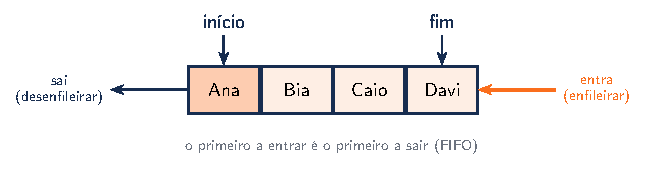
\includegraphics[width=0.85\linewidth,keepaspectratio]{imagens/capitulo-04_fila.pdf}
\end{center}

\begin{center}
\begin{tabular}{@{}p{0.3\linewidth}p{0.42\linewidth}p{0.14\linewidth}@{}}
\toprule
\rowcolor{headergray}
\tblheader{Operação} & \tblheader{O que faz} & \tblheader{Custo} \\
\midrule
\texttt{enfileirar(v)} & coloca \texttt{v} no fim (\textit{enqueue}) & $O(1)$ \\
\rowcolor{rowgray} \texttt{desenfileirar()} & retira e devolve o início (\textit{dequeue}) & $O(1)$ \\
\texttt{frente()} & devolve o início sem retirar & $O(1)$ \\
\rowcolor{rowgray} \texttt{vazia()} & diz se não há elementos & $O(1)$ \\
\bottomrule
\end{tabular}
\end{center}

\subsection{4.6 Fila com nós encadeados}

A lista encadeada com ponteiro para o fim (Capítulo 3) já tem tudo que a fila precisa: inserir no fim e remover do início, ambos em $O(1)$.

\begin{codigo}
\begin{Verbatim}[breaklines=true, breaksymbolleft={}, fontsize=\footnotesize]
#include <stdexcept>

template <typename T>
class Fila {
private:
    struct No {
        T valor;
        No *proximo;
    };
    No *inicio = nullptr;   // de onde sai
    No *fim = nullptr;      // por onde entra
    int tamanho = 0;

public:
    Fila() = default;
    ~Fila() {
        while (!vazia()) {
            desenfileirar();
        }
    }
    Fila(const Fila &) = delete;
    Fila &operator=(const Fila &) = delete;

    bool vazia() const { return inicio == nullptr; }
    int quantidade() const { return tamanho; }

    void enfileirar(const T &valor) {
        No *novo = new No{valor, nullptr};
        if (fim == nullptr) {
            inicio = novo;          // fila vazia: o novo é o primeiro
        } else {
            fim->proximo = novo;    // entra atrás do último
        }
        fim = novo;
        tamanho++;
    }

    T desenfileirar() {
        if (vazia()) {
            throw runtime_error("fila vazia");
        }
        No *velho = inicio;
        T valor = velho->valor;
        inicio = inicio->proximo;
        if (inicio == nullptr) {
            fim = nullptr;          // a fila ficou vazia
        }
        delete velho;
        tamanho--;
        return valor;
    }

    const T &frente() const {
        if (vazia()) {
            throw runtime_error("fila vazia");
        }
        return inicio->valor;
    }
};

int main() {
    Fila<string> atendimento;
    atendimento.enfileirar("Ana");
    atendimento.enfileirar("Bia");
    atendimento.enfileirar("Caio");

    cout << "Proximo a ser atendido: " << atendimento.frente() << endl;  // Ana
    while (!atendimento.vazia()) {
        cout << "Atendendo " << atendimento.desenfileirar() << endl;     // Ana, Bia, Caio
    }
}
\end{Verbatim}
\end{codigo}

Repare no cuidado em \texttt{desenfileirar}: quando o último elemento sai, \texttt{fim} também precisa voltar a \texttt{nullptr}. Se isso for esquecido, o próximo \texttt{enfileirar} vai ligar o novo nó a um nó que já foi apagado.

\subsection{4.7 Fila circular em vetor}

Também é possível fazer uma fila com um vetor de tamanho fixo, o que evita alocar um nó a cada inserção. A ideia ingênua seria remover sempre da posição 0 e deslocar os demais elementos, mas isso custaria $O(n)$ a cada saída.

A solução é a \textbf{fila circular}: em vez de mover os elementos, movemos os índices. \texttt{inicio} indica onde está o primeiro elemento e \texttt{fim} indica onde entra o próximo. Quando um índice passa da última posição, ele volta para a posição 0, como se o vetor fosse um anel. Quem faz essa volta é o operador de resto da divisão, \texttt{\%}.

\begin{center}
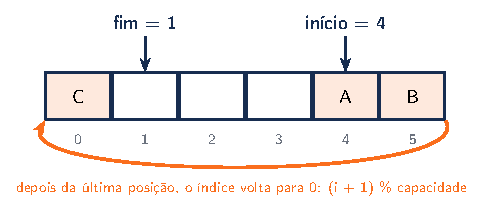
\includegraphics[width=0.9\linewidth,keepaspectratio]{imagens/capitulo-04_fila_circular.pdf}
\end{center}

Na figura, a fila tem capacidade 6 e contém, na ordem de saída, A (posição 4), B (posição 5) e C (posição 0). O próximo elemento entrará na posição 1.

\begin{codigo}
\begin{Verbatim}[breaklines=true, breaksymbolleft={}, fontsize=\footnotesize]
#include <stdexcept>

template <typename T>
class FilaCircular {
private:
    T *dados;
    int capacidade;
    int inicio = 0;    // posição do primeiro elemento
    int fim = 0;       // posição onde entra o próximo
    int tamanho = 0;

public:
    explicit FilaCircular(int cap) : dados(new T[cap]), capacidade(cap) {}
    ~FilaCircular() { delete[] dados; }
    FilaCircular(const FilaCircular &) = delete;
    FilaCircular &operator=(const FilaCircular &) = delete;

    bool vazia() const { return tamanho == 0; }
    bool cheia() const { return tamanho == capacidade; }

    bool enfileirar(const T &valor) {
        if (cheia()) {
            return false;                     // não há espaço
        }
        dados[fim] = valor;
        fim = (fim + 1) % capacidade;         // depois da última, volta para 0
        tamanho++;
        return true;
    }

    T desenfileirar() {
        if (vazia()) {
            throw runtime_error("fila vazia");
        }
        T valor = dados[inicio];
        inicio = (inicio + 1) % capacidade;
        tamanho--;
        return valor;
    }
};

int main() {
    FilaCircular<int> f(6);
    for (int v = 1; v <= 6; v++) {
        f.enfileirar(v);                         // ocupa as posições 0 a 5
    }
    cout << boolalpha << f.enfileirar(7) << endl;  // false: está cheia

    cout << f.desenfileirar() << " ";            // 1
    cout << f.desenfileirar() << endl;           // 2

    f.enfileirar(7);                             // entra na posição 0 (deu a volta)
    f.enfileirar(8);                             // entra na posição 1
    while (!f.vazia()) {
        cout << f.desenfileirar() << " ";        // 3 4 5 6 7 8
    }
    cout << endl;
}
\end{Verbatim}
\end{codigo}

A fila circular faz todas as operações em $O(1)$ e não aloca memória a cada inserção, mas tem capacidade fixa. É muito usada em sistemas que recebem dados continuamente, como teclados, placas de rede e players de áudio, onde é chamada de \textit{buffer} circular.

\subsection{4.8 Aplicações da fila}

\begin{itemize}
  \item \textbf{Atendimento por ordem de chegada}: senhas de banco, pedidos de uma lanchonete, chamados de suporte.
  \item \textbf{Fila de impressão}: os documentos são impressos na ordem em que foram enviados.
  \item \textbf{Escalonamento de processos}: o sistema operacional reveza o processador entre os programas usando filas.
  \item \textbf{Busca em largura em grafos}: no Capítulo 6, a fila vai garantir que um grafo seja explorado em camadas, primeiro os vizinhos mais próximos.
\end{itemize}

\subsection{4.9 Pilhas e filas prontas}

A biblioteca padrão do C++ oferece \texttt{stack} (pilha), \texttt{queue} (fila) e \texttt{deque}, uma fila de duas pontas que permite inserir e remover no início e no fim. Atenção a um detalhe: no C++, \texttt{pop()} retira o elemento, mas \textbf{não o devolve}. Para ler o valor, use \texttt{top()} (pilha) ou \texttt{front()} (fila) antes de chamar \texttt{pop()}.

\begin{codigo}
\begin{Verbatim}[breaklines=true, breaksymbolleft={}, fontsize=\footnotesize]
#include <stack>
#include <queue>

int main() {
    stack<int> pilha;
    pilha.push(10);
    pilha.push(20);
    cout << pilha.top() << endl;    // 20: lê o topo
    pilha.pop();                    // retira, sem devolver

    queue<string> fila;
    fila.push("Ana");
    fila.push("Bia");
    cout << fila.front() << endl;   // Ana: lê o início
    fila.pop();
    cout << fila.size() << endl;    // 1
}
\end{Verbatim}
\end{codigo}

\begin{destaque}{Comparando com Python}
Em Python, a própria \texttt{list} funciona bem como pilha, porque \texttt{append} e \texttt{pop} no fim custam $O(1)$. Para fila, porém, \textbf{não} use a lista: \texttt{lista.pop(0)} desloca todos os elementos e custa $O(n)$. Use o \texttt{deque}:

\begin{codigo}
\begin{Verbatim}[breaklines=true, breaksymbolleft={}, fontsize=\footnotesize]
from collections import deque

pilha = []
pilha.append(10)
pilha.append(20)
print(pilha.pop())        # 20, O(1)

fila = deque()
fila.append("Ana")        # enfileirar, O(1)
fila.append("Bia")
print(fila.popleft())     # Ana, desenfileirar em O(1)
\end{Verbatim}
\end{codigo}
\end{destaque}

\subsection{Erros Comuns}

\begin{itemize}
  \item \textbf{Desempilhar ou desenfileirar uma estrutura vazia.} Sempre verifique \texttt{vazia()} antes, ou trate a exceção. Na STL do C++, chamar \texttt{top()} ou \texttt{pop()} em uma pilha vazia tem comportamento indefinido.
  \item \textbf{Esperar que o \texttt{pop()} da STL devolva o valor.} Ele só retira. Leia com \texttt{top()} ou \texttt{front()} antes.
  \item \textbf{Inverter a ordem dos operandos.} Na pós-fixa, o primeiro valor desempilhado é o \textit{segundo} operando: em \texttt{8 2 -}, a conta é $8 - 2$, não $2 - 8$.
  \item \textbf{Não zerar o \texttt{fim} quando a fila esvazia.} Ao retirar o último elemento, \texttt{fim} deve voltar a \texttt{nullptr}.
  \item \textbf{Esquecer o resto da divisão na fila circular.} Sem \texttt{\% capacidade}, o índice passa do fim do vetor e o programa escreve fora da memória reservada.
  \item \textbf{Confundir fila cheia com fila vazia.} Na fila circular, \texttt{inicio == fim} acontece nos dois casos. Por isso guardamos o \texttt{tamanho}.
  \item \textbf{Usar \texttt{lista.pop(0)} como fila em Python.} Cada saída custa $O(n)$; com muitos elementos, o programa fica lento. Use \texttt{deque}.
\end{itemize}

\newpage
\section{Capítulo 5 -- Árvores}

Listas, pilhas e filas são estruturas \textbf{lineares}: cada elemento tem, no máximo, um anterior e um seguinte. Muitos dados do mundo real, porém, não são assim. As pastas do seu computador, o organograma de uma empresa e a estrutura de uma página HTML são \textbf{hierárquicos}: um item contém outros, que contêm outros. Neste capítulo você vai estudar a estrutura que representa hierarquias, a \textbf{árvore}, e uma de suas versões mais úteis, a \textbf{árvore binária de busca}, que permite procurar um valor entre milhões em poucas comparações.

\subsection{5.1 Organização hierárquica}

Uma árvore é formada por \textbf{nós} ligados por \textbf{arestas}. Existe um nó especial no topo, a \textbf{raiz}, e cada um dos outros nós tem exatamente um nó acima dele. Diferente das árvores da natureza, na computação a raiz é desenhada em cima e a árvore cresce para baixo.

Um bom exemplo é a expressão $(3 + 5) \cdot 4 - 2$. O operador que é calculado por último, o $-$, fica na raiz; seus dois operandos ficam abaixo dele, e assim por diante, até os números, que ficam nas pontas:

\begin{center}
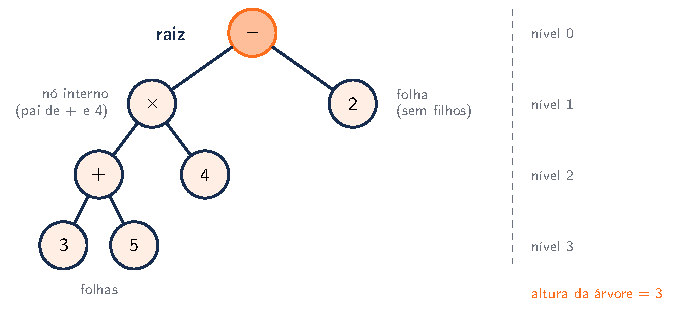
\includegraphics[width=0.85\linewidth,keepaspectratio]{imagens/capitulo-05_termos.pdf}
\end{center}

Repare que os parênteses desapareceram: a própria forma da árvore diz que a soma acontece antes da multiplicação, porque ela está mais embaixo. Os termos abaixo serão usados em todo o capítulo:

\begin{center}
\begin{tabular}{@{}p{0.24\linewidth}p{0.68\linewidth}@{}}
\toprule
\rowcolor{headergray}
\tblheader{Termo} & \tblheader{Significado} \\
\midrule
raiz & o único nó sem pai; no exemplo, o $-$ \\
\rowcolor{rowgray} pai e filho & se uma aresta liga A (acima) a B (abaixo), A é o pai e B é o filho \\
irmãos & nós com o mesmo pai, como o $+$ e o 4 \\
\rowcolor{rowgray} folha & nó sem filhos; no exemplo, os números 3, 5, 4 e 2 \\
nó interno & nó que tem pelo menos um filho \\
\rowcolor{rowgray} subárvore & um nó junto com todos os seus descendentes; ela também é uma árvore \\
caminho & sequência de nós ligados por arestas, de cima para baixo \\
\rowcolor{rowgray} nível (profundidade) & número de arestas da raiz até o nó; a raiz está no nível 0 \\
altura & maior nível da árvore, ou seja, o caminho mais longo da raiz até uma folha \\
\rowcolor{rowgray} grau & número de filhos de um nó \\
\bottomrule
\end{tabular}
\end{center}

\begin{destaque}{Por que a árvore é recursiva}
Cada filho da raiz é, ele mesmo, a raiz de uma árvore menor. Essa é a ideia mais importante do capítulo: \textbf{uma árvore é uma raiz ligada a subárvores}. Por isso quase todas as funções sobre árvores são recursivas e muito curtas: elas resolvem o problema para a raiz e deixam a recursão resolver para as subárvores, como você praticou no Capítulo 1.
\end{destaque}

\subsection{5.2 A árvore binária}

Quando cada nó tem \textbf{no máximo dois filhos}, a árvore é chamada de \textbf{binária}. Os filhos são distinguidos pela posição: o filho da \textbf{esquerda} e o filho da \textbf{direita}. A árvore da expressão é binária, porque cada operador tem exatamente dois operandos.

O nó de uma árvore binária lembra o nó da lista duplamente encadeada do Capítulo 3: um valor e dois ponteiros. A diferença está no significado dos ponteiros, que agora apontam para \textbf{baixo}:

\begin{codigo}
\begin{Verbatim}[breaklines=true, breaksymbolleft={}, fontsize=\footnotesize]
// trecho
struct No {
    string valor;
    No *esquerda;
    No *direita;
};

No *novo(const string &valor, No *esquerda = nullptr, No *direita = nullptr) {
    return new No{valor, esquerda, direita};
}
\end{Verbatim}
\end{codigo}

Um ponteiro \texttt{nullptr} significa ``não há filho deste lado''. Uma folha tem os dois ponteiros nulos, e a árvore inteira é acessada a partir de um único ponteiro para a raiz, assim como a lista era acessada pelo ponteiro para o início.

Alguns formatos de árvore binária recebem nomes próprios:

\begin{itemize}
  \item \textbf{Estritamente binária}: todo nó tem zero ou dois filhos, nunca um só. A árvore da expressão é estritamente binária.
  \item \textbf{Cheia}: estritamente binária e com todas as folhas no mesmo nível. Uma árvore cheia de altura $h$ tem $2^{h+1} - 1$ nós.
  \item \textbf{Completa}: todos os níveis estão cheios, exceto talvez o último, que é preenchido da esquerda para a direita. Você vai reencontrar esse formato no Capítulo 8, no \textit{heapsort}.
\end{itemize}

A conta da árvore cheia mostra algo valioso: com altura 9, cabem $2^{10} - 1 = 1023$ nós; com altura 19, mais de um milhão. Uma árvore bem formada é \textbf{baixa}, mesmo com muitos nós. Guarde essa ideia para a Seção 5.5.

\subsection{5.3 Percorrendo uma árvore}

Percorrer uma estrutura é visitar cada elemento uma vez. Na lista existe uma só ordem natural, do início ao fim. Na árvore binária, em cada nó há três coisas a fazer (visitar o próprio nó, percorrer a subárvore esquerda e percorrer a direita), e a ordem escolhida dá nome ao percurso:

\begin{itemize}
  \item \textbf{Pré-ordem}: primeiro o nó, depois a esquerda, depois a direita.
  \item \textbf{Em ordem} (ou ordem simétrica): primeiro a esquerda, depois o nó, depois a direita.
  \item \textbf{Pós-ordem}: primeiro a esquerda, depois a direita, por último o nó.
\end{itemize}

As três funções são idênticas, mudando apenas a posição da linha que imprime:

\begin{codigo}
\begin{Verbatim}[breaklines=true, breaksymbolleft={}, fontsize=\footnotesize]
// trecho
void preOrdem(No *no) {
    if (no == nullptr) return;     // árvore vazia: nada a fazer
    cout << no->valor << " ";      // 1. o próprio nó
    preOrdem(no->esquerda);        // 2. subárvore esquerda
    preOrdem(no->direita);         // 3. subárvore direita
}

void emOrdem(No *no) {
    if (no == nullptr) return;
    emOrdem(no->esquerda);
    cout << no->valor << " ";
    emOrdem(no->direita);
}

void posOrdem(No *no) {
    if (no == nullptr) return;
    posOrdem(no->esquerda);
    posOrdem(no->direita);
    cout << no->valor << " ";
}
\end{Verbatim}
\end{codigo}

Aplicados à árvore da expressão, os percursos produzem:

\begin{center}
\begin{tabular}{@{}p{0.22\linewidth}p{0.3\linewidth}p{0.4\linewidth}@{}}
\toprule
\rowcolor{headergray}
\tblheader{Percurso} & \tblheader{Resultado} & \tblheader{Observação} \\
\midrule
pré-ordem & \texttt{- * + 3 5 4 2} & operador antes dos operandos (notação prefixa) \\
\rowcolor{rowgray} em ordem & \texttt{3 + 5 * 4 - 2} & a forma como escrevemos, mas sem os parênteses \\
pós-ordem & \texttt{3 5 + 4 * 2 -} & a notação pós-fixa do Capítulo 4 \\
\rowcolor{rowgray} em largura & \texttt{- * 2 + 4 3 5} & nível por nível, da esquerda para a direita \\
\bottomrule
\end{tabular}
\end{center}

A pós-ordem gerou exatamente a notação que a pilha do Capítulo 4 sabia calcular. E o percurso em ordem perdeu os parênteses: se você quiser a expressão correta, basta imprimir um ``('' antes da subárvore esquerda e um ``)'' depois da direita.

O último percurso da tabela, \textbf{em largura}, não é recursivo: ele visita a raiz, depois todos os nós do nível 1, depois os do nível 2, e assim por diante. Para isso, usa uma \textbf{fila}: cada nó visitado coloca seus filhos no final da fila, e eles serão visitados depois de todos os nós que já estavam esperando. É o FIFO do Capítulo 4 trabalhando a favor da árvore.

O programa completo monta a árvore da expressão, faz os quatro percursos e usa a mesma ideia recursiva para calcular a altura, contar as folhas e até \textbf{avaliar} a expressão:

\begin{codigo}
\begin{Verbatim}[breaklines=true, breaksymbolleft={}, fontsize=\footnotesize]
#include <algorithm>   // max
#include <queue>

struct No {
    string valor;
    No *esquerda;
    No *direita;
};

No *novo(const string &valor, No *esquerda = nullptr, No *direita = nullptr) {
    return new No{valor, esquerda, direita};
}

void preOrdem(No *no) {
    if (no == nullptr) return;     // árvore vazia: nada a fazer
    cout << no->valor << " ";      // 1. o próprio nó
    preOrdem(no->esquerda);        // 2. subárvore esquerda
    preOrdem(no->direita);         // 3. subárvore direita
}

void emOrdem(No *no) {
    if (no == nullptr) return;
    emOrdem(no->esquerda);
    cout << no->valor << " ";
    emOrdem(no->direita);
}

void posOrdem(No *no) {
    if (no == nullptr) return;
    posOrdem(no->esquerda);
    posOrdem(no->direita);
    cout << no->valor << " ";
}

void emLargura(No *raiz) {
    if (raiz == nullptr) return;
    queue<No *> fila;
    fila.push(raiz);
    while (!fila.empty()) {
        No *atual = fila.front();
        fila.pop();
        cout << atual->valor << " ";
        if (atual->esquerda != nullptr) fila.push(atual->esquerda);
        if (atual->direita != nullptr) fila.push(atual->direita);
    }
}

int altura(No *no) {
    if (no == nullptr) return -1;  // árvore vazia: assim, uma folha tem altura 0
    return 1 + max(altura(no->esquerda), altura(no->direita));
}

int contarFolhas(No *no) {
    if (no == nullptr) return 0;
    if (no->esquerda == nullptr && no->direita == nullptr) return 1;
    return contarFolhas(no->esquerda) + contarFolhas(no->direita);
}

double avaliar(No *no) {
    if (no->esquerda == nullptr && no->direita == nullptr) {
        return stod(no->valor);    // folha: é um número
    }
    double a = avaliar(no->esquerda);
    double b = avaliar(no->direita);
    if (no->valor == "+") return a + b;
    if (no->valor == "-") return a - b;
    if (no->valor == "*") return a * b;
    return a / b;
}

void liberar(No *no) {
    if (no == nullptr) return;
    liberar(no->esquerda);         // pós-ordem: os filhos antes do pai
    liberar(no->direita);
    delete no;
}

int main() {
    // (3 + 5) * 4 - 2
    No *raiz = novo("-",
                    novo("*",
                         novo("+", novo("3"), novo("5")),
                         novo("4")),
                    novo("2"));

    cout << "Pré-ordem:  "; preOrdem(raiz);  cout << endl;  // - * + 3 5 4 2
    cout << "Em ordem:   "; emOrdem(raiz);   cout << endl;  // 3 + 5 * 4 - 2
    cout << "Pós-ordem:  "; posOrdem(raiz);  cout << endl;  // 3 5 + 4 * 2 -
    cout << "Em largura: "; emLargura(raiz); cout << endl;  // - * 2 + 4 3 5

    cout << "Altura: " << altura(raiz) << endl;            // 3
    cout << "Folhas: " << contarFolhas(raiz) << endl;      // 4
    cout << "Valor: " << avaliar(raiz) << endl;            // 30

    liberar(raiz);
}
\end{Verbatim}
\end{codigo}

Repare em \texttt{liberar}: ela é uma pós-ordem. Os filhos precisam ser apagados \textbf{antes} do pai, porque depois do \texttt{delete} do pai os ponteiros para os filhos não podem mais ser lidos. Todos os percursos visitam cada nó uma única vez, então custam $O(n)$.

\subsection{5.4 Árvore binária de busca}

Na lista encadeada, procurar um valor exige olhar os elementos um a um: $O(n)$. A \textbf{árvore binária de busca} (ABB, ou BST, do inglês \textit{binary search tree}) organiza os valores de forma que cada comparação descarte uma parte inteira da árvore. Para isso, ela segue uma única regra, válida em \textbf{todos} os nós:

\begin{itemize}
  \item todos os valores da subárvore \textbf{esquerda} são \textbf{menores} que o valor do nó;
  \item todos os valores da subárvore \textbf{direita} são \textbf{maiores} que o valor do nó.
\end{itemize}

\begin{center}
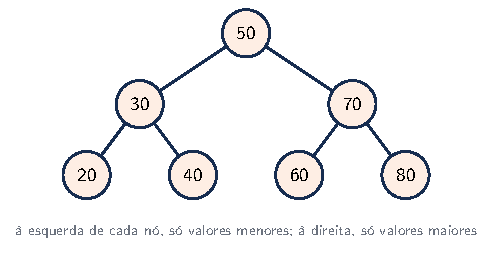
\includegraphics[width=0.62\linewidth,keepaspectratio]{imagens/capitulo-05_abb.pdf}
\end{center}

\subsubsection{Buscar}

Para procurar o 60 na árvore acima, compare com a raiz: 60 é maior que 50, então ele só pode estar à direita. Agora compare com o 70: 60 é menor, então desça à esquerda. Achou. Foram três comparações, e a metade esquerda da árvore nem foi olhada. É a mesma ideia da \textbf{busca binária} em um vetor ordenado, que você verá no Capítulo 7, só que agora em uma estrutura que aceita inserções e remoções.

\begin{codigo}
\begin{Verbatim}[breaklines=true, breaksymbolleft={}, fontsize=\footnotesize]
// trecho
    bool contem(int valor) const {
        No *atual = raiz;
        while (atual != nullptr) {
            if (valor == atual->valor) return true;
            atual = (valor < atual->valor) ? atual->esquerda : atual->direita;
        }
        return false;
    }
\end{Verbatim}
\end{codigo}

O \textbf{menor} valor da árvore é o nó mais à esquerda, e o \textbf{maior} é o nó mais à direita: basta descer sempre para o mesmo lado até não haver mais filho.

\subsubsection{Inserir}

Inserir é buscar o lugar onde o valor deveria estar. Quando a busca chega a um ponteiro nulo, é ali que o novo nó entra, sempre como \textbf{folha}. A versão recursiva fica curta: ela recebe a raiz de uma subárvore, insere o valor do lado certo e devolve a raiz, que muda apenas quando a subárvore estava vazia.

\begin{codigo}
\begin{Verbatim}[breaklines=true, breaksymbolleft={}, fontsize=\footnotesize]
// trecho
    static No *inserir(No *no, int valor) {
        if (no == nullptr) {
            return new No{valor};           // achou o lugar: nova folha
        }
        if (valor < no->valor) {
            no->esquerda = inserir(no->esquerda, valor);
        } else if (valor > no->valor) {
            no->direita = inserir(no->direita, valor);
        }
        // valor igual: já está na árvore, nada a fazer
        return no;
    }
\end{Verbatim}
\end{codigo}

A linha \texttt{no->esquerda = inserir(no->esquerda, valor)} é o truque que evita casos especiais: ela reconecta o filho, quer ele tenha mudado (era nulo e virou o nó novo), quer não. Esta implementação não guarda valores repetidos; quando for preciso, cada nó pode ter um contador de ocorrências.

\subsubsection{Percorrer em ordem}

Pela regra da ABB, o percurso em ordem visita primeiro todos os menores, depois o nó, depois todos os maiores. O resultado é que ele imprime os valores \textbf{ordenados}. Na árvore da figura: \texttt{20 30 40 50 60 70 80}. Uma ABB, portanto, é também uma forma de manter dados sempre em ordem.

\subsubsection{Remover}

A remoção é a operação mais delicada, porque o nó removido pode ter filhos que precisam continuar na árvore. Há três casos:

\begin{enumerate}
  \item \textbf{O nó é uma folha.} Basta apagá-lo e deixar nulo o ponteiro do pai.
  \item \textbf{O nó tem um filho.} O filho ocupa o lugar dele: o pai passa a apontar diretamente para o neto. A regra da ABB continua valendo, porque toda a subárvore do filho estava do mesmo lado do pai.
  \item \textbf{O nó tem dois filhos.} Nenhum dos filhos pode simplesmente subir, pois o outro ficaria sem lugar. A solução é encontrar o \textbf{sucessor}: o menor valor da subárvore direita. Ele é maior que tudo à esquerda e menor que todo o resto à direita, então pode ocupar o lugar do nó removido. Copiamos o valor do sucessor para o nó e removemos o sucessor lá de baixo, o que cai no caso 1 ou 2, já que o sucessor não tem filho à esquerda.
\end{enumerate}

\begin{center}
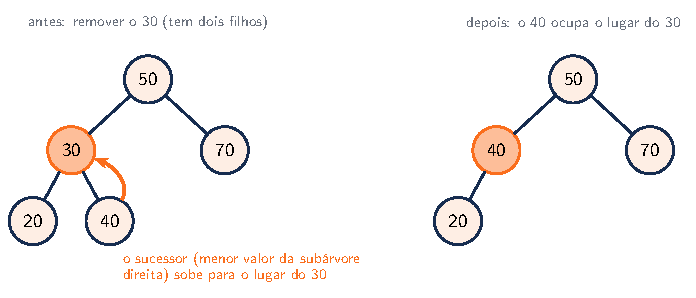
\includegraphics[width=0.85\linewidth,keepaspectratio]{imagens/capitulo-05_remocao.pdf}
\end{center}

\begin{codigo}
\begin{Verbatim}[breaklines=true, breaksymbolleft={}, fontsize=\footnotesize]
// trecho
    static No *remover(No *no, int valor) {
        if (no == nullptr) {
            return nullptr;                 // o valor não está na árvore
        }
        if (valor < no->valor) {
            no->esquerda = remover(no->esquerda, valor);
        } else if (valor > no->valor) {
            no->direita = remover(no->direita, valor);
        } else if (no->esquerda == nullptr) {   // casos 1 e 2: no máximo um filho
            No *filho = no->direita;
            delete no;
            return filho;
        } else if (no->direita == nullptr) {
            No *filho = no->esquerda;
            delete no;
            return filho;
        } else {                                // caso 3: dois filhos
            No *sucessor = no->direita;
            while (sucessor->esquerda != nullptr) {
                sucessor = sucessor->esquerda;
            }
            no->valor = sucessor->valor;        // o sucessor sobe
            no->direita = remover(no->direita, sucessor->valor);  // e sai lá de baixo
        }
        return no;
    }
\end{Verbatim}
\end{codigo}

Os casos 1 e 2 foram tratados juntos: se não há filho à esquerda, quem sobe é o da direita, e se este também for nulo, o pai simplesmente recebe \texttt{nullptr}. O programa completo aparece no final da próxima seção.

\subsection{5.5 Árvores balanceadas e degeneradas}

Buscar, inserir e remover descem um único caminho da raiz até, no máximo, uma folha. O custo dessas operações é, então, $O(h)$, em que $h$ é a altura da árvore. A questão é: qual é a altura?

Depende da \textbf{ordem de inserção}. As mesmas cinco chaves podem formar árvores muito diferentes:

\begin{center}
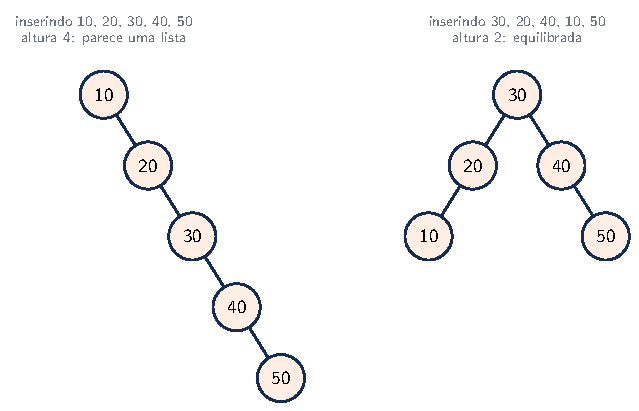
\includegraphics[width=0.8\linewidth,keepaspectratio]{imagens/capitulo-05_degenerada.pdf}
\end{center}

Quando os valores chegam já ordenados, cada novo nó vira filho direito do anterior, e a árvore \textbf{degenera} em algo igual a uma lista encadeada: altura $n - 1$ e busca $O(n)$. Quando a árvore está \textbf{balanceada}, isto é, com as subárvores de cada nó de alturas parecidas, a altura fica perto de $\log_2 n$, como você viu na conta da árvore cheia.

O experimento abaixo insere os números de 1 a 1000 de duas formas: em ordem crescente, e começando sempre pelo elemento do meio de cada intervalo:

\begin{codigo}
\begin{Verbatim}[breaklines=true, breaksymbolleft={}, fontsize=\footnotesize]
// trecho
void inserirDoMeio(ArvoreBusca &arvore, int inicio, int fim) {
    if (inicio > fim) return;
    int meio = (inicio + fim) / 2;
    arvore.inserir(meio);
    inserirDoMeio(arvore, inicio, meio - 1);
    inserirDoMeio(arvore, meio + 1, fim);
}

    ArvoreBusca crescente, equilibrada;
    for (int v = 1; v <= 1000; v++) {
        crescente.inserir(v);
    }
    inserirDoMeio(equilibrada, 1, 1000);
    cout << "Altura (crescente): " << crescente.altura() << endl;     // 999
    cout << "Altura (do meio): " << equilibrada.altura() << endl;     // 9
\end{Verbatim}
\end{codigo}

São os mesmos mil valores. Em uma árvore, achar o último exige percorrer mil nós; na outra, no máximo dez.

\begin{center}
\begin{tabular}{@{}p{0.26\linewidth}p{0.3\linewidth}p{0.3\linewidth}@{}}
\toprule
\rowcolor{headergray}
\tblheader{Operação} & \tblheader{ABB balanceada} & \tblheader{ABB degenerada} \\
\midrule
buscar & $O(\log n)$ & $O(n)$ \\
\rowcolor{rowgray} inserir & $O(\log n)$ & $O(n)$ \\
remover & $O(\log n)$ & $O(n)$ \\
\rowcolor{rowgray} mínimo e máximo & $O(\log n)$ & $O(n)$ \\
percorrer tudo & $O(n)$ & $O(n)$ \\
\bottomrule
\end{tabular}
\end{center}

Este é o programa completo da árvore binária de busca, com o experimento das alturas:

\begin{codigo}
\begin{Verbatim}[breaklines=true, breaksymbolleft={}, fontsize=\footnotesize]
#include <algorithm>   // max
#include <stdexcept>   // runtime_error

class ArvoreBusca {
private:
    struct No {
        int valor;
        No *esquerda = nullptr;
        No *direita = nullptr;
    };
    No *raiz = nullptr;

    static No *inserir(No *no, int valor) {
        if (no == nullptr) {
            return new No{valor};           // achou o lugar: nova folha
        }
        if (valor < no->valor) {
            no->esquerda = inserir(no->esquerda, valor);
        } else if (valor > no->valor) {
            no->direita = inserir(no->direita, valor);
        }
        // valor igual: já está na árvore, nada a fazer
        return no;
    }

    static No *remover(No *no, int valor) {
        if (no == nullptr) {
            return nullptr;                 // o valor não está na árvore
        }
        if (valor < no->valor) {
            no->esquerda = remover(no->esquerda, valor);
        } else if (valor > no->valor) {
            no->direita = remover(no->direita, valor);
        } else if (no->esquerda == nullptr) {   // casos 1 e 2: no máximo um filho
            No *filho = no->direita;
            delete no;
            return filho;
        } else if (no->direita == nullptr) {
            No *filho = no->esquerda;
            delete no;
            return filho;
        } else {                                // caso 3: dois filhos
            No *sucessor = no->direita;
            while (sucessor->esquerda != nullptr) {
                sucessor = sucessor->esquerda;
            }
            no->valor = sucessor->valor;        // o sucessor sobe
            no->direita = remover(no->direita, sucessor->valor);  // e sai lá de baixo
        }
        return no;
    }

    static void emOrdem(No *no) {
        if (no == nullptr) return;
        emOrdem(no->esquerda);
        cout << no->valor << " ";
        emOrdem(no->direita);
    }

    static int altura(No *no) {
        if (no == nullptr) return -1;
        return 1 + max(altura(no->esquerda), altura(no->direita));
    }

    static void liberar(No *no) {
        if (no == nullptr) return;
        liberar(no->esquerda);
        liberar(no->direita);
        delete no;
    }

public:
    ArvoreBusca() = default;
    ~ArvoreBusca() { liberar(raiz); }
    ArvoreBusca(const ArvoreBusca &) = delete;
    ArvoreBusca &operator=(const ArvoreBusca &) = delete;

    void inserir(int valor) { raiz = inserir(raiz, valor); }
    void remover(int valor) { raiz = remover(raiz, valor); }

    bool contem(int valor) const {
        No *atual = raiz;
        while (atual != nullptr) {
            if (valor == atual->valor) return true;
            atual = (valor < atual->valor) ? atual->esquerda : atual->direita;
        }
        return false;
    }

    int minimo() const {
        if (raiz == nullptr) throw runtime_error("árvore vazia");
        No *atual = raiz;
        while (atual->esquerda != nullptr) atual = atual->esquerda;
        return atual->valor;
    }

    int maximo() const {
        if (raiz == nullptr) throw runtime_error("árvore vazia");
        No *atual = raiz;
        while (atual->direita != nullptr) atual = atual->direita;
        return atual->valor;
    }

    int altura() const { return altura(raiz); }
    void imprimir() const { emOrdem(raiz); cout << endl; }
};

void inserirDoMeio(ArvoreBusca &arvore, int inicio, int fim) {
    if (inicio > fim) return;
    int meio = (inicio + fim) / 2;
    arvore.inserir(meio);
    inserirDoMeio(arvore, inicio, meio - 1);
    inserirDoMeio(arvore, meio + 1, fim);
}

int main() {
    ArvoreBusca arvore;
    for (int v : {50, 30, 70, 20, 40, 60, 80}) {
        arvore.inserir(v);
    }
    arvore.imprimir();                                   // 20 30 40 50 60 70 80
    cout << boolalpha << arvore.contem(60) << endl;      // true
    cout << arvore.contem(65) << endl;                   // false
    cout << arvore.minimo() << " " << arvore.maximo() << endl;  // 20 80
    cout << "Altura: " << arvore.altura() << endl;       // 2

    arvore.remover(30);   // dois filhos: o sucessor 40 sobe
    arvore.remover(40);   // agora o 40 tem um filho só, o 20
    arvore.remover(80);   // folha
    arvore.imprimir();                                   // 20 50 60 70

    ArvoreBusca crescente, equilibrada;
    for (int v = 1; v <= 1000; v++) {
        crescente.inserir(v);
    }
    inserirDoMeio(equilibrada, 1, 1000);
    cout << "Altura (crescente): " << crescente.altura() << endl;     // 999
    cout << "Altura (do meio): " << equilibrada.altura() << endl;     // 9
}
\end{Verbatim}
\end{codigo}

As funções recursivas ficaram \texttt{private} e \texttt{static}: quem usa a classe chama \texttt{inserir(valor)} sem precisar saber que existem nós, e a versão interna recebe a subárvore em que deve trabalhar. É o mesmo encapsulamento da pilha e da fila do Capítulo 4.

\subsection{5.6 Árvores AVL}

Na prática, você raramente controla a ordem em que os dados chegam. Cadastros por data, códigos sequenciais e nomes já ordenados são comuns, e são justamente o pior caso da ABB. A solução é uma árvore que \textbf{se rebalanceia sozinha} a cada inserção. A primeira delas, e a mais conhecida, é a \textbf{árvore AVL}, nome que vem das iniciais de seus criadores, Adelson-Velsky e Landis.

\subsubsection{Fator de balanceamento}

Cada nó da AVL guarda a própria altura. Com ela, calcula-se o \textbf{fator de balanceamento}:

\[ \text{fator} = \text{altura da subárvore esquerda} - \text{altura da subárvore direita} \]

A AVL exige que, em \textbf{todos} os nós, o fator seja $-1$, $0$ ou $+1$. Fator $+2$ significa que o nó pesa demais à esquerda; $-2$, que pesa demais à direita. Essa regra garante que a altura da AVL nunca passa de cerca de $1{,}44 \log_2 n$, então todas as operações ficam em $O(\log n)$.

\subsubsection{Rotações}

Quando uma inserção deixa algum nó com fator $\pm 2$, a árvore é consertada com uma \textbf{rotação}: uma troca de poucos ponteiros que faz um filho subir e o pai descer, \textbf{mantendo a regra da ABB}.

\begin{center}
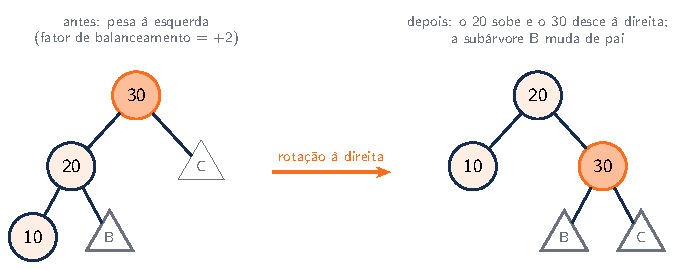
\includegraphics[width=0.85\linewidth,keepaspectratio]{imagens/capitulo-05_rotacao.pdf}
\end{center}

Na rotação à direita da figura, o 20 sobe e o 30 vira seu filho direito. A subárvore B, que estava à direita do 20, tem valores entre 20 e 30; por isso ela passa a ficar à esquerda do 30, e a ordem continua correta. A rotação à esquerda é o espelho dessa.

Há quatro situações de desequilíbrio, nomeadas pelo caminho do nó desequilibrado até o ponto onde entrou o novo valor:

\begin{center}
\begin{tabular}{@{}p{0.24\linewidth}p{0.3\linewidth}p{0.38\linewidth}@{}}
\toprule
\rowcolor{headergray}
\tblheader{Caso} & \tblheader{Como identificar} & \tblheader{Correção} \\
\midrule
esquerda-esquerda & fator $+2$, filho esquerdo com fator $\ge 0$ & rotação simples à direita \\
\rowcolor{rowgray} direita-direita & fator $-2$, filho direito com fator $\le 0$ & rotação simples à esquerda \\
esquerda-direita & fator $+2$, filho esquerdo com fator $-1$ & rotação dupla: à esquerda no filho, depois à direita no nó \\
\rowcolor{rowgray} direita-esquerda & fator $-2$, filho direito com fator $+1$ & rotação dupla: à direita no filho, depois à esquerda no nó \\
\bottomrule
\end{tabular}
\end{center}

Nos casos ``em linha'' (esquerda-esquerda e direita-direita), uma rotação basta. Nos casos ``em zigue-zague'', a primeira rotação endireita o zigue-zague, transformando-o no caso em linha, e a segunda resolve. Por exemplo, ao inserir 30, 10 e 20, o 20 entra à direita do 10, que está à esquerda do 30: é o caso esquerda-direita, e o resultado final tem o 20 na raiz.

\subsubsection{Inserção na AVL}

A inserção é a mesma da ABB, com um passo a mais: na volta da recursão, cada nó do caminho atualiza sua altura e, se precisar, é rebalanceado. Como a recursão volta de baixo para cima, o primeiro nó desequilibrado encontrado é o mais próximo da inserção, que é exatamente o que deve ser corrigido.

\begin{codigo}
\begin{Verbatim}[breaklines=true, breaksymbolleft={}, fontsize=\footnotesize]
#include <algorithm>   // max

struct NoAVL {
    int valor;
    int altura = 0;                // uma folha tem altura 0
    NoAVL *esquerda = nullptr;
    NoAVL *direita = nullptr;
};

int altura(NoAVL *no) { return no == nullptr ? -1 : no->altura; }

int fator(NoAVL *no) { return altura(no->esquerda) - altura(no->direita); }

void atualizar(NoAVL *no) {
    no->altura = 1 + max(altura(no->esquerda), altura(no->direita));
}

NoAVL *rotacaoDireita(NoAVL *y) {
    NoAVL *x = y->esquerda;
    NoAVL *b = x->direita;
    x->direita = y;                // y desce para a direita de x
    y->esquerda = b;               // a subárvore B muda de pai
    atualizar(y);                  // y primeiro, porque agora está embaixo
    atualizar(x);
    return x;                      // x é a nova raiz desta subárvore
}

NoAVL *rotacaoEsquerda(NoAVL *x) {
    NoAVL *y = x->direita;
    NoAVL *b = y->esquerda;
    y->esquerda = x;
    x->direita = b;
    atualizar(x);
    atualizar(y);
    return y;
}

NoAVL *balancear(NoAVL *no) {
    atualizar(no);
    int f = fator(no);
    if (f > 1) {                                   // pesa à esquerda
        if (fator(no->esquerda) < 0) {             // zigue-zague: esquerda-direita
            no->esquerda = rotacaoEsquerda(no->esquerda);
        }
        return rotacaoDireita(no);
    }
    if (f < -1) {                                  // pesa à direita
        if (fator(no->direita) > 0) {              // zigue-zague: direita-esquerda
            no->direita = rotacaoDireita(no->direita);
        }
        return rotacaoEsquerda(no);
    }
    return no;                                     // já está equilibrado
}

NoAVL *inserir(NoAVL *no, int valor) {
    if (no == nullptr) return new NoAVL{valor};
    if (valor < no->valor) {
        no->esquerda = inserir(no->esquerda, valor);
    } else if (valor > no->valor) {
        no->direita = inserir(no->direita, valor);
    } else {
        return no;                                 // repetido: nada muda
    }
    return balancear(no);                          // conserta na volta da recursão
}

void preOrdem(NoAVL *no) {
    if (no == nullptr) return;
    cout << no->valor << " ";
    preOrdem(no->esquerda);
    preOrdem(no->direita);
}

void liberar(NoAVL *no) {
    if (no == nullptr) return;
    liberar(no->esquerda);
    liberar(no->direita);
    delete no;
}

int main() {
    NoAVL *raiz = nullptr;
    for (int v : {30, 10, 20}) {                   // caso esquerda-direita
        raiz = inserir(raiz, v);
    }
    preOrdem(raiz); cout << endl;                  // 20 10 30
    liberar(raiz);

    raiz = nullptr;
    for (int v = 1; v <= 7; v++) {                 // em ordem crescente
        raiz = inserir(raiz, v);
    }
    preOrdem(raiz); cout << endl;                  // 4 2 1 3 6 5 7
    cout << "Altura: " << altura(raiz) << endl;    // 2
    liberar(raiz);

    raiz = nullptr;
    for (int v = 1; v <= 1000; v++) {
        raiz = inserir(raiz, v);
    }
    cout << "Altura com 1000: " << altura(raiz) << endl;   // 9
    liberar(raiz);
}
\end{Verbatim}
\end{codigo}

Inserir de 1 a 7 em ordem crescente, que na ABB comum produziria uma ``lista'' de altura 6, gera na AVL uma árvore cheia de altura 2, com o 4 na raiz. E os mil valores crescentes, que deixaram a ABB com altura 999, ficam com altura 9. Cada rotação custa $O(1)$, pois mexe em poucos ponteiros, e há no máximo uma correção (simples ou dupla) por inserção; o custo total continua $O(\log n)$.

A remoção na AVL segue a mesma ideia: remove-se como na ABB e chama-se \texttt{balancear} na volta da recursão. A diferença é que, na remoção, pode ser preciso rebalancear vários nós no caminho até a raiz.

\begin{destaque}{Outras árvores balanceadas}
A AVL não é a única. A \textbf{árvore rubro-negra} (\textit{red-black tree}) usa uma regra mais folgada, baseada em cores nos nós, e faz menos rotações nas inserções e remoções; ela é a base do \texttt{std::set} e do \texttt{std::map} do C++. Já as \textbf{árvores B} têm nós com muitos filhos e são usadas em bancos de dados e sistemas de arquivos, em que cada nó corresponde a um bloco do disco.
\end{destaque}

\subsection{5.7 Árvores prontas}

Em projetos reais, você usará as árvores balanceadas da biblioteca padrão. O \texttt{std::set} guarda valores sem repetição e o \texttt{std::map} guarda pares chave-valor; ambos mantêm os elementos \textbf{ordenados} e fazem inserção, busca e remoção em $O(\log n)$.

\begin{codigo}
\begin{Verbatim}[breaklines=true, breaksymbolleft={}, fontsize=\footnotesize]
#include <set>
#include <map>

int main() {
    set<int> numeros = {50, 30, 70, 20, 40};
    numeros.insert(60);
    numeros.insert(30);                     // repetido: ignorado
    numeros.erase(70);
    for (int n : numeros) {
        cout << n << " ";                   // sempre em ordem
    }
    cout << endl;                           // 20 30 40 50 60
    cout << numeros.count(40) << endl;      // 1: está no conjunto

    map<string, int> idades;
    idades["Caio"] = 20;
    idades["Ana"] = 19;
    idades["Bia"] = 21;
    for (const auto &[nome, idade] : idades) {
        cout << nome << ": " << idade << endl;  // Ana: 19, Bia: 21, Caio: 20
    }
}
\end{Verbatim}
\end{codigo}

\begin{destaque}{Comparando com Python}
Python não tem uma árvore de busca na biblioteca padrão. O \texttt{dict} e o \texttt{set} usam \textbf{tabelas hash}, que buscam em $O(1)$ em média, mas não guardam as chaves em ordem: para percorrê-las ordenadas, é preciso chamar \texttt{sorted}, que custa $O(n \log n)$ a cada vez. Quando a ordem importa, você pode escrever sua própria árvore, e o código fica parecido com o do C++, sem ponteiros explícitos nem \texttt{delete}, porque o coletor de lixo libera os nós:

\begin{codigo}
\begin{Verbatim}[breaklines=true, breaksymbolleft={}, fontsize=\footnotesize]
class No:
    def __init__(self, valor):
        self.valor = valor
        self.esquerda = None
        self.direita = None

def inserir(no, valor):
    if no is None:
        return No(valor)
    if valor < no.valor:
        no.esquerda = inserir(no.esquerda, valor)
    elif valor > no.valor:
        no.direita = inserir(no.direita, valor)
    return no

def em_ordem(no):
    if no is not None:
        yield from em_ordem(no.esquerda)
        yield no.valor
        yield from em_ordem(no.direita)

raiz = None
for v in [50, 30, 70, 20, 40]:
    raiz = inserir(raiz, v)
print(list(em_ordem(raiz)))    # [20, 30, 40, 50, 70]
\end{Verbatim}
\end{codigo}
\end{destaque}

\subsection{Erros Comuns}

\begin{itemize}
  \item \textbf{Esquecer o caso da árvore vazia.} Toda função recursiva sobre árvores precisa começar testando \texttt{nullptr}. Sem isso, a recursão acessa um ponteiro nulo ao chegar abaixo de uma folha.
  \item \textbf{Não reconectar o filho na inserção recursiva.} Chamar apenas \texttt{inserir(no->esquerda, valor)}, sem atribuir o resultado a \texttt{no->esquerda}, cria o nó novo e o perde: ele nunca é ligado à árvore e a memória vaza.
  \item \textbf{Liberar o pai antes dos filhos.} Depois do \texttt{delete} de um nó, seus ponteiros não podem mais ser lidos. Libere sempre em pós-ordem.
  \item \textbf{Conferir a regra da ABB só com os filhos diretos.} A regra vale para a subárvore inteira: um valor 55 na subárvore esquerda do 50 quebra a árvore, mesmo que ele seja menor que o pai imediato.
  \item \textbf{Escolher o sucessor errado na remoção.} O sucessor é o \textit{menor} valor da subárvore \textit{direita} (desça uma vez à direita e depois sempre à esquerda). Também funciona usar o \textit{maior} da subárvore esquerda, mas não misture as duas ideias.
  \item \textbf{Supor que a ABB é sempre $O(\log n)$.} Isso só vale se ela estiver balanceada. Com dados ordenados, uma ABB comum vira uma lista.
  \item \textbf{Atualizar as alturas na ordem errada na rotação.} O nó que desceu deve ser atualizado antes do que subiu, porque a altura do novo pai depende da altura do novo filho.
  \item \textbf{Esperar ordem do \texttt{dict} ou do \texttt{set} do Python.} O \texttt{dict} preserva a ordem de inserção, não a ordem das chaves, e o \texttt{set} não garante ordem nenhuma.
\end{itemize}

\newpage
\section{Capítulo 6 -- Grafos}

A árvore do Capítulo 5 representa hierarquias: cada nó tem um único pai. Muitas relações, porém, não têm hierarquia nenhuma. Uma cidade se liga a várias outras por estradas, uma pessoa é amiga de várias outras, uma página da web aponta para muitas páginas, e todas podem formar ciclos. A estrutura que representa qualquer rede de ligações é o \textbf{grafo}. Neste capítulo você vai aprender a guardar um grafo na memória, a percorrê-lo e a resolver dois problemas clássicos: encontrar o caminho mais curto e ligar todos os pontos com o menor custo.

\subsection{6.1 Vértices e arestas}

Um grafo é formado por um conjunto de \textbf{vértices} (os pontos) e um conjunto de \textbf{arestas} (as ligações entre pares de vértices). Uma árvore é um caso particular de grafo: um grafo conectado e sem ciclos.

As arestas podem ter ou não um sentido:

\begin{center}
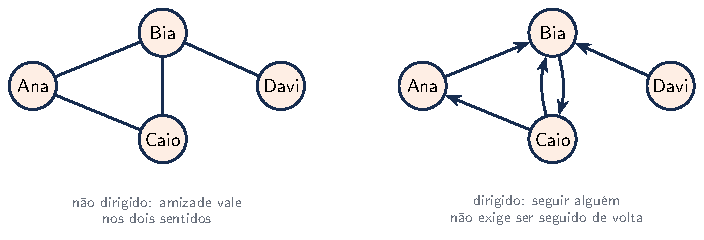
\includegraphics[width=0.9\linewidth,keepaspectratio]{imagens/capitulo-06_tipos.pdf}
\end{center}

\begin{itemize}
  \item Em um grafo \textbf{não dirigido}, a aresta liga os dois vértices nos dois sentidos, como uma amizade ou uma estrada de mão dupla.
  \item Em um grafo \textbf{dirigido} (ou \textbf{dígrafo}), cada aresta tem origem e destino e é desenhada como uma seta, como ``seguir'' alguém em uma rede social ou um pré-requisito entre disciplinas.
\end{itemize}

Quando cada aresta tem um número associado, como uma distância, um tempo ou um custo, o grafo é \textbf{ponderado}, e esse número é o \textbf{peso} da aresta. O grafo abaixo será usado como exemplo em todo o capítulo: seis cidades e as estradas entre elas, com as distâncias em quilômetros.

\begin{center}
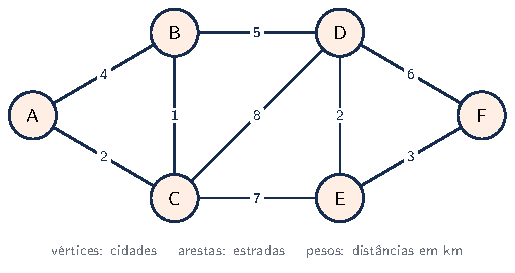
\includegraphics[width=0.8\linewidth,keepaspectratio]{imagens/capitulo-06_grafo.pdf}
\end{center}

\begin{center}
\begin{tabular}{@{}p{0.24\linewidth}p{0.68\linewidth}@{}}
\toprule
\rowcolor{headergray}
\tblheader{Termo} & \tblheader{Significado} \\
\midrule
adjacentes (vizinhos) & dois vértices ligados por uma aresta; no exemplo, B e D \\
\rowcolor{rowgray} grau & número de arestas de um vértice; o grau de C é 4 \\
caminho & sequência de vértices em que cada um é vizinho do seguinte, como A, C, E, F \\
\rowcolor{rowgray} ciclo & caminho que começa e termina no mesmo vértice, como A, B, C, A \\
conexo & grafo em que existe caminho entre quaisquer dois vértices \\
\rowcolor{rowgray} componente conexo & cada ``pedaço'' de um grafo que não é conexo \\
\bottomrule
\end{tabular}
\end{center}

Nos algoritmos, é costume chamar o número de vértices de $V$ e o número de arestas de $E$ (do inglês \textit{edges}). O exemplo tem $V = 6$ e $E = 9$.

\subsection{6.2 Representando um grafo}

Existem duas formas principais de guardar um grafo na memória. Para numerá-los, os vértices recebem índices: A é 0, B é 1, e assim por diante.

\subsubsection{Matriz de adjacência}

A \textbf{matriz de adjacência} é uma tabela $V \times V$ em que a posição \texttt{[i][j]} diz se existe aresta de \texttt{i} para \texttt{j} (ou guarda o peso dela). No grafo de amizades da primeira figura:

\begin{codigo}
\begin{Verbatim}[breaklines=true, breaksymbolleft={}, fontsize=\footnotesize]
int main() {
    const int N = 4;
    const string nomes[N] = {"Ana", "Bia", "Caio", "Davi"};
    bool amigos[N][N] = {};                  // começa tudo false

    amigos[0][1] = amigos[1][0] = true;      // Ana e Bia
    amigos[0][2] = amigos[2][0] = true;      // Ana e Caio
    amigos[1][2] = amigos[2][1] = true;      // Bia e Caio
    amigos[1][3] = amigos[3][1] = true;      // Bia e Davi

    cout << boolalpha << amigos[0][3] << endl;   // false: consulta em O(1)

    for (int v = 0; v < N; v++) {
        int grau = 0;
        for (int u = 0; u < N; u++) {        // percorre a linha inteira: O(V)
            if (amigos[v][u]) grau++;
        }
        cout << nomes[v] << ": " << grau << endl;   // Ana: 2, Bia: 3, Caio: 2, Davi: 1
    }
}
\end{Verbatim}
\end{codigo}

Em um grafo não dirigido, a matriz é \textbf{simétrica}: cada aresta é marcada duas vezes. A vantagem é saber em $O(1)$ se dois vértices são vizinhos. A desvantagem é a memória: são sempre $V^2$ posições, mesmo que haja poucas arestas. Uma rede social com um milhão de pessoas precisaria de um trilhão de posições, quase todas \texttt{false}.

\subsubsection{Lista de adjacência}

A \textbf{lista de adjacência} guarda, para cada vértice, apenas a lista dos seus vizinhos. Em C++, a forma mais simples é um \texttt{vector} de \texttt{vector}s: a posição \texttt{v} contém os vizinhos de \texttt{v}, cada um com o peso da aresta.

\begin{codigo}
\begin{Verbatim}[breaklines=true, breaksymbolleft={}, fontsize=\footnotesize]
// trecho
struct Aresta {
    int destino;
    int peso;
};

class Grafo {
private:
    vector<vector<Aresta>> adjacentes;   // uma lista de vizinhos por vértice

public:
    explicit Grafo(int n) : adjacentes(n) {}

    int vertices() const { return static_cast<int>(adjacentes.size()); }

    void ligar(int a, int b, int peso = 1) {   // aresta não dirigida
        adjacentes[a].push_back({b, peso});
        adjacentes[b].push_back({a, peso});
    }

    const vector<Aresta> &vizinhos(int v) const { return adjacentes[v]; }
};
\end{Verbatim}
\end{codigo}

Repare que não há \texttt{new} nem \texttt{delete}: o \texttt{vector} cuida da própria memória e a libera sozinho quando o grafo deixa de existir. Para um grafo dirigido, basta \texttt{ligar} acrescentar só a primeira das duas linhas.

\begin{center}
\begin{tabular}{@{}p{0.36\linewidth}p{0.26\linewidth}p{0.26\linewidth}@{}}
\toprule
\rowcolor{headergray}
\tblheader{Operação} & \tblheader{Matriz} & \tblheader{Lista} \\
\midrule
memória & $O(V^2)$ & $O(V + E)$ \\
\rowcolor{rowgray} existe aresta entre u e v? & $O(1)$ & $O(\text{grau de u})$ \\
percorrer os vizinhos de v & $O(V)$ & $O(\text{grau de v})$ \\
\rowcolor{rowgray} percorrer o grafo inteiro & $O(V^2)$ & $O(V + E)$ \\
\bottomrule
\end{tabular}
\end{center}

A maioria dos grafos reais é \textbf{esparsa}: cada vértice tem poucos vizinhos em comparação com o total. Por isso a lista de adjacência é a escolha padrão, e é a que usaremos no resto do capítulo. A matriz compensa em grafos pequenos ou \textbf{densos}, com quase todas as arestas possíveis.

\subsection{6.3 Busca em largura}

Percorrer um grafo é mais delicado do que percorrer uma árvore, por dois motivos: não existe uma raiz natural, e os ciclos fazem um vértice ser alcançável por vários caminhos. Para não visitar o mesmo vértice duas vezes, nem entrar em um ciclo infinito, os percursos \textbf{marcam} cada vértice já descoberto.

A \textbf{busca em largura} (BFS, do inglês \textit{breadth-first search}) é a generalização do percurso em largura da árvore. Ela parte de um vértice de origem, descobre todos os seus vizinhos, depois os vizinhos dos vizinhos, e assim por diante, em camadas. Assim como na árvore, quem organiza as camadas é uma \textbf{fila}.

\begin{center}
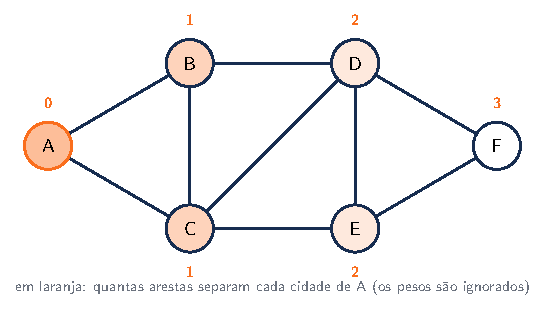
\includegraphics[width=0.8\linewidth,keepaspectratio]{imagens/capitulo-06_largura.pdf}
\end{center}

Como cada camada fica uma aresta mais longe da origem, a BFS calcula, de brinde, o \textbf{menor número de arestas} entre a origem e cada vértice. Em um mapa sem distâncias, ou em uma rede social (``quantos amigos de amigos separam duas pessoas?''), esse é exatamente o caminho mais curto.

\begin{codigo}
\begin{Verbatim}[breaklines=true, breaksymbolleft={}, fontsize=\footnotesize]
// trecho
vector<int> largura(const Grafo &g, int origem, vector<int> &pai) {
    vector<int> distancia(g.vertices(), -1);   // -1: ainda não descoberto
    pai.assign(g.vertices(), -1);
    queue<int> fila;
    distancia[origem] = 0;
    fila.push(origem);
    while (!fila.empty()) {
        int v = fila.front();
        fila.pop();
        for (const Aresta &a : g.vizinhos(v)) {
            if (distancia[a.destino] == -1) {   // primeira vez que aparece
                distancia[a.destino] = distancia[v] + 1;
                pai[a.destino] = v;             // foi descoberto a partir de v
                fila.push(a.destino);
            }
        }
    }
    return distancia;
}
\end{Verbatim}
\end{codigo}

O vetor \texttt{distancia} faz o papel da marcação: $-1$ significa ``ainda não descoberto''. O vetor \texttt{pai} guarda de qual vértice cada um foi descoberto; seguindo os pais a partir de qualquer vértice, você refaz o caminho até a origem. As arestas \texttt{pai}--filho formam uma árvore, chamada \textbf{árvore de busca}.

Cada vértice entra na fila uma única vez, e a lista de vizinhos de cada um é percorrida uma única vez. O custo total é $O(V + E)$.

\subsection{6.4 Busca em profundidade}

A \textbf{busca em profundidade} (DFS, do inglês \textit{depth-first search}) faz o contrário: em vez de avançar em camadas, ela segue um caminho até não haver mais para onde ir e só então volta para tentar outra direção, como alguém explorando um labirinto com a mão sempre na parede. Ela é naturalmente recursiva, e a pilha que guarda o caminho de volta é a própria pilha de execução do Capítulo 4.

\begin{codigo}
\begin{Verbatim}[breaklines=true, breaksymbolleft={}, fontsize=\footnotesize]
// trecho
void profundidade(const Grafo &g, int v, vector<bool> &visitado, vector<int> &pai) {
    visitado[v] = true;
    for (const Aresta &a : g.vizinhos(v)) {
        if (!visitado[a.destino]) {
            pai[a.destino] = v;
            profundidade(g, a.destino, visitado, pai);   // mergulha antes de olhar o próximo vizinho
        }
    }
}
\end{Verbatim}
\end{codigo}

Partindo de A no grafo das cidades, as duas buscas descobrem os mesmos vértices, mas por caminhos bem diferentes. As arestas das árvores de busca mostram isso:

\begin{center}
\begin{tabular}{@{}p{0.28\linewidth}p{0.3\linewidth}p{0.34\linewidth}@{}}
\toprule
\rowcolor{headergray}
\tblheader{Busca} & \tblheader{Árvore de busca} & \tblheader{Formato} \\
\midrule
largura (BFS) & A-B, A-C, B-D, C-E, D-F & larga e baixa: altura 3 \\
\rowcolor{rowgray} profundidade (DFS) & A-B, B-C, C-D, D-E, E-F & um único caminho: altura 5 \\
\bottomrule
\end{tabular}
\end{center}

A DFS também custa $O(V + E)$ e serve de base para muitos algoritmos. Um dos mais simples é \textbf{contar os componentes conexos}: chame a DFS a partir de cada vértice ainda não visitado; cada chamada feita pelo laço principal descobre um componente inteiro.

\begin{codigo}
\begin{Verbatim}[breaklines=true, breaksymbolleft={}, fontsize=\footnotesize]
// trecho
int contarComponentes(const Grafo &g) {
    vector<bool> visitado(g.vertices(), false);
    vector<int> pai(g.vertices(), -1);
    int componentes = 0;
    for (int v = 0; v < g.vertices(); v++) {
        if (!visitado[v]) {                    // começa um grupo novo
            componentes++;
            profundidade(g, v, visitado, pai);
        }
    }
    return componentes;
}
\end{Verbatim}
\end{codigo}

O programa completo monta o grafo das cidades, executa as duas buscas e conta os componentes de uma rede com três grupos separados:

\begin{codigo}
\begin{Verbatim}[breaklines=true, breaksymbolleft={}, fontsize=\footnotesize]
#include <vector>
#include <queue>

struct Aresta {
    int destino;
    int peso;
};

class Grafo {
private:
    vector<vector<Aresta>> adjacentes;   // uma lista de vizinhos por vértice

public:
    explicit Grafo(int n) : adjacentes(n) {}

    int vertices() const { return static_cast<int>(adjacentes.size()); }

    void ligar(int a, int b, int peso = 1) {   // aresta não dirigida
        adjacentes[a].push_back({b, peso});
        adjacentes[b].push_back({a, peso});
    }

    const vector<Aresta> &vizinhos(int v) const { return adjacentes[v]; }
};

const string NOMES = "ABCDEF";

vector<int> largura(const Grafo &g, int origem, vector<int> &pai) {
    vector<int> distancia(g.vertices(), -1);   // -1: ainda não descoberto
    pai.assign(g.vertices(), -1);
    queue<int> fila;
    distancia[origem] = 0;
    fila.push(origem);
    while (!fila.empty()) {
        int v = fila.front();
        fila.pop();
        for (const Aresta &a : g.vizinhos(v)) {
            if (distancia[a.destino] == -1) {   // primeira vez que aparece
                distancia[a.destino] = distancia[v] + 1;
                pai[a.destino] = v;             // foi descoberto a partir de v
                fila.push(a.destino);
            }
        }
    }
    return distancia;
}

void profundidade(const Grafo &g, int v, vector<bool> &visitado, vector<int> &pai) {
    visitado[v] = true;
    for (const Aresta &a : g.vizinhos(v)) {
        if (!visitado[a.destino]) {
            pai[a.destino] = v;
            profundidade(g, a.destino, visitado, pai);   // mergulha antes de olhar o próximo vizinho
        }
    }
}

int contarComponentes(const Grafo &g) {
    vector<bool> visitado(g.vertices(), false);
    vector<int> pai(g.vertices(), -1);
    int componentes = 0;
    for (int v = 0; v < g.vertices(); v++) {
        if (!visitado[v]) {                    // começa um grupo novo
            componentes++;
            profundidade(g, v, visitado, pai);
        }
    }
    return componentes;
}

void mostrarArvoreDeBusca(const vector<int> &pai) {
    for (int v = 0; v < static_cast<int>(pai.size()); v++) {
        if (pai[v] != -1) {
            cout << NOMES[pai[v]] << "-" << NOMES[v] << " ";
        }
    }
    cout << endl;
}

int main() {
    enum { A, B, C, D, E, F };
    Grafo mapa(6);
    mapa.ligar(A, B, 4);
    mapa.ligar(A, C, 2);
    mapa.ligar(B, C, 1);
    mapa.ligar(B, D, 5);
    mapa.ligar(C, D, 8);
    mapa.ligar(C, E, 7);
    mapa.ligar(D, E, 2);
    mapa.ligar(D, F, 6);
    mapa.ligar(E, F, 3);

    vector<int> pai;
    vector<int> distancia = largura(mapa, A, pai);
    for (int v = 0; v < mapa.vertices(); v++) {
        cout << NOMES[v] << "=" << distancia[v] << " ";
    }
    cout << endl;                  // A=0 B=1 C=1 D=2 E=2 F=3
    mostrarArvoreDeBusca(pai);     // A-B A-C B-D C-E D-F

    vector<bool> visitado(mapa.vertices(), false);
    pai.assign(mapa.vertices(), -1);
    profundidade(mapa, A, visitado, pai);
    mostrarArvoreDeBusca(pai);     // A-B B-C C-D D-E E-F

    Grafo rede(7);                 // grupos {0, 1, 2}, {3, 4} e {5, 6}
    rede.ligar(0, 1);
    rede.ligar(1, 2);
    rede.ligar(3, 4);
    rede.ligar(5, 6);
    cout << contarComponentes(rede) << " componentes" << endl;   // 3 componentes
}
\end{Verbatim}
\end{codigo}

O \texttt{enum} dentro do \texttt{main} dá nomes aos índices: \texttt{A} vale 0, \texttt{B} vale 1, e assim por diante. Isso deixa as chamadas a \texttt{ligar} tão legíveis quanto a figura.

\subsubsection{Ordenação topológica}

Uma aplicação importante dos grafos dirigidos é decidir uma ordem que respeite dependências: em que ordem cursar disciplinas com pré-requisitos, compilar arquivos que dependem uns dos outros ou executar as etapas de um projeto. Essa ordem se chama \textbf{ordenação topológica}, e só existe se o grafo não tiver ciclos (um grafo dirigido sem ciclos é chamado de DAG, do inglês \textit{directed acyclic graph}).

Um jeito simples de calculá-la, conhecido como algoritmo de Kahn, usa uma fila: conte quantos pré-requisitos faltam para cada vértice; os que não têm nenhum podem ser feitos já e entram na fila. Cada vez que um vértice sai da fila, ele é ``cumprido'' e diminui a contagem dos que dependem dele; quem chegar a zero entra na fila.

\begin{codigo}
\begin{Verbatim}[breaklines=true, breaksymbolleft={}, fontsize=\footnotesize]
#include <vector>
#include <queue>

vector<int> ordemTopologica(const vector<vector<int>> &depois) {
    int n = static_cast<int>(depois.size());
    vector<int> faltam(n, 0);               // pré-requisitos ainda não cumpridos
    for (const vector<int> &lista : depois) {
        for (int v : lista) faltam[v]++;
    }
    queue<int> prontas;
    for (int v = 0; v < n; v++) {
        if (faltam[v] == 0) prontas.push(v);
    }
    vector<int> ordem;
    while (!prontas.empty()) {
        int v = prontas.front();
        prontas.pop();
        ordem.push_back(v);
        for (int w : depois[v]) {
            faltam[w]--;
            if (faltam[w] == 0) prontas.push(w);   // último pré-requisito cumprido
        }
    }
    return ordem;                           // se faltou alguém, havia um ciclo
}

int main() {
    const vector<string> disciplinas = {"Algoritmos I", "Algoritmos II", "Banco de Dados",
                                        "Programação Web", "Engenharia de Software", "Projeto Final"};
    enum { ALG1, ALG2, BD, WEB, ENG, PROJ };
    vector<vector<int>> depois(6);          // depois[a]: disciplinas que exigem a
    depois[ALG1] = {ALG2, BD};
    depois[ALG2] = {WEB, ENG};
    depois[BD] = {WEB};
    depois[WEB] = {PROJ};
    depois[ENG] = {PROJ};

    for (int d : ordemTopologica(depois)) {
        cout << disciplinas[d] << endl;
    }
    // Algoritmos I, Algoritmos II, Banco de Dados,
    // Engenharia de Software, Programação Web, Projeto Final

    depois[PROJ] = {ALG1};                  // erro de cadastro: cria um ciclo
    cout << ordemTopologica(depois).size() << " de 6" << endl;   // 0 de 6
}
\end{Verbatim}
\end{codigo}

Quando há um ciclo, os vértices do ciclo esperam uns pelos outros e nunca chegam a zero. Por isso o algoritmo também serve para \textbf{detectar ciclos}: se a ordem tiver menos vértices que o grafo, existe uma dependência circular.

\subsection{6.5 Caminho mínimo: algoritmo de Dijkstra}

A BFS encontra o caminho com menos \textbf{arestas}, mas no mapa das cidades isso não basta: de A até F, o caminho A, B, D, F tem só três estradas e soma $4 + 5 + 6 = 15$ km, enquanto A, C, E, F também tem três e soma 12 km. Quando as arestas têm pesos, o caminho mínimo é o de menor \textbf{soma de pesos}, e o algoritmo clássico para encontrá-lo foi criado por Edsger Dijkstra.

A ideia é parecida com a da BFS, trocando a fila comum por uma \textbf{fila de prioridade}, que sempre entrega o vértice com a \textbf{menor distância conhecida} até o momento:

\begin{enumerate}
  \item A origem começa com distância 0; todos os outros, com ``infinito''.
  \item Retire da fila o vértice \texttt{v} com a menor distância. Essa distância é definitiva: como os pesos não são negativos, nenhum outro caminho pode ficar mais curto passando por vértices mais distantes.
  \item Para cada vizinho de \texttt{v}, verifique se chegar a ele passando por \texttt{v} é mais curto do que o melhor caminho conhecido. Se for, atualize a distância (isso se chama \textbf{relaxar} a aresta) e coloque o vizinho na fila.
  \item Repita até a fila esvaziar.
\end{enumerate}

\begin{center}
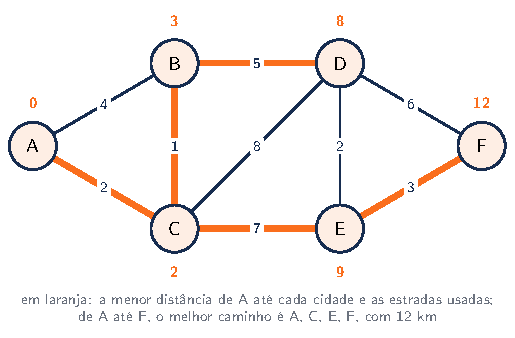
\includegraphics[width=0.8\linewidth,keepaspectratio]{imagens/capitulo-06_dijkstra.pdf}
\end{center}

A fila de prioridade do C++ é a \texttt{priority\_queue}. Por padrão ela entrega o \textbf{maior} elemento; com \texttt{greater<>}, passa a entregar o menor. Guardamos pares (distância, vértice), porque os pares são comparados primeiro pelo primeiro campo. Por dentro, ela é um \textit{heap}, estrutura que você vai construir no Capítulo 8, e insere e retira em $O(\log n)$.

\begin{codigo}
\begin{Verbatim}[breaklines=true, breaksymbolleft={}, fontsize=\footnotesize]
// trecho
vector<int> dijkstra(const Grafo &g, int origem, vector<int> &anterior) {
    vector<int> distancia(g.vertices(), INFINITO);
    anterior.assign(g.vertices(), -1);
    priority_queue<pair<int, int>, vector<pair<int, int>>, greater<>> fila;   // (distância, vértice)
    distancia[origem] = 0;
    fila.push({0, origem});
    while (!fila.empty()) {
        auto [d, v] = fila.top();               // o mais próximo ainda na fila
        fila.pop();
        if (d > distancia[v]) continue;         // registro antigo: já achamos caminho melhor
        for (const Aresta &a : g.vizinhos(v)) {
            int nova = d + a.peso;
            if (nova < distancia[a.destino]) {  // relaxa a aresta
                distancia[a.destino] = nova;
                anterior[a.destino] = v;
                fila.push({nova, a.destino});
            }
        }
    }
    return distancia;
}
\end{Verbatim}
\end{codigo}

Um vértice pode entrar na fila mais de uma vez, sempre que sua distância melhora. A linha \texttt{if (d > distancia[v]) continue;} descarta as entradas antigas, que ficaram desatualizadas. Com lista de adjacência e \textit{heap}, o custo é $O((V + E) \log V)$.

\begin{destaque}{Pesos negativos}
O Dijkstra só funciona com pesos \textbf{maiores ou iguais a zero}. Com um peso negativo, um vértice já tratado como definitivo poderia ficar mais perto depois, por um caminho que passa pela aresta negativa, e o algoritmo não volta para corrigir. Para esses grafos existe o algoritmo de Bellman-Ford, mais lento: $O(V \cdot E)$.
\end{destaque}

\subsection{6.6 Árvore geradora mínima}

Agora o problema é outro. A prefeitura quer asfaltar estradas de modo que seja possível ir de qualquer cidade a qualquer outra, gastando o mínimo possível. Não é preciso asfaltar todas: basta escolher um conjunto de estradas que \textbf{conecte todos os vértices} com a \textbf{menor soma de pesos}. Esse conjunto não terá ciclos (um ciclo sempre tem uma estrada dispensável), então será uma árvore com $V - 1$ arestas, chamada \textbf{árvore geradora mínima} (AGM, ou MST, do inglês \textit{minimum spanning tree}).

\begin{center}
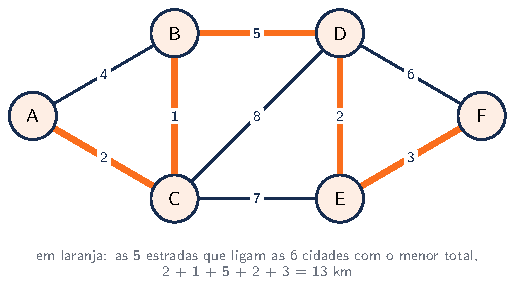
\includegraphics[width=0.8\linewidth,keepaspectratio]{imagens/capitulo-06_agm.pdf}
\end{center}

Compare com a figura do Dijkstra: as respostas são diferentes. A AGM usa a estrada D-E e não a C-E, porque o objetivo dela é o menor \textbf{total} da rede, e não o menor caminho a partir de uma cidade. Para ir de A até F pela AGM, você percorreria $2 + 1 + 5 + 2 + 3 = 13$ km, mais do que os 12 km do Dijkstra.

O \textbf{algoritmo de Prim} constrói a AGM a partir de um vértice qualquer. A cada passo, ele escolhe a aresta \textbf{mais barata} que liga a árvore já construída a um vértice ainda de fora. É, de novo, um trabalho para a fila de prioridade, agora guardando (peso, de onde, para onde):

\begin{codigo}
\begin{Verbatim}[breaklines=true, breaksymbolleft={}, fontsize=\footnotesize]
// trecho
int prim(const Grafo &g, vector<pair<int, int>> &escolhidas) {
    vector<bool> naArvore(g.vertices(), false);
    priority_queue<tuple<int, int, int>, vector<tuple<int, int, int>>, greater<>> fila;   // (peso, de, para)
    fila.push({0, -1, 0});                      // começa pelo vértice 0, sem aresta
    int total = 0;
    while (!fila.empty()) {
        auto [peso, de, v] = fila.top();        // a aresta mais barata disponível
        fila.pop();
        if (naArvore[v]) continue;              // criaria um ciclo
        naArvore[v] = true;
        total += peso;
        if (de != -1) escolhidas.push_back({de, v});
        for (const Aresta &a : g.vizinhos(v)) {
            if (!naArvore[a.destino]) fila.push({a.peso, v, a.destino});
        }
    }
    return total;
}
\end{Verbatim}
\end{codigo}

O Prim é um \textbf{algoritmo guloso}: a cada passo, faz a escolha que parece melhor naquele momento, sem voltar atrás, e mesmo assim chega à melhor resposta. Você vai estudar essa família de algoritmos no Capítulo 9, junto com o \textbf{algoritmo de Kruskal}, outra forma gulosa de construir a AGM. O custo do Prim com \textit{heap} também é $O((V + E) \log V)$.

Este é o programa completo dos dois algoritmos:

\begin{codigo}
\begin{Verbatim}[breaklines=true, breaksymbolleft={}, fontsize=\footnotesize]
#include <vector>
#include <queue>
#include <tuple>
#include <limits>       // numeric_limits
#include <functional>   // greater
#include <algorithm>    // reverse

struct Aresta {
    int destino;
    int peso;
};

class Grafo {
private:
    vector<vector<Aresta>> adjacentes;   // uma lista de vizinhos por vértice

public:
    explicit Grafo(int n) : adjacentes(n) {}

    int vertices() const { return static_cast<int>(adjacentes.size()); }

    void ligar(int a, int b, int peso = 1) {   // aresta não dirigida
        adjacentes[a].push_back({b, peso});
        adjacentes[b].push_back({a, peso});
    }

    const vector<Aresta> &vizinhos(int v) const { return adjacentes[v]; }
};

const string NOMES = "ABCDEF";
const int INFINITO = numeric_limits<int>::max();

vector<int> dijkstra(const Grafo &g, int origem, vector<int> &anterior) {
    vector<int> distancia(g.vertices(), INFINITO);
    anterior.assign(g.vertices(), -1);
    priority_queue<pair<int, int>, vector<pair<int, int>>, greater<>> fila;   // (distância, vértice)
    distancia[origem] = 0;
    fila.push({0, origem});
    while (!fila.empty()) {
        auto [d, v] = fila.top();               // o mais próximo ainda na fila
        fila.pop();
        if (d > distancia[v]) continue;         // registro antigo: já achamos caminho melhor
        for (const Aresta &a : g.vizinhos(v)) {
            int nova = d + a.peso;
            if (nova < distancia[a.destino]) {  // relaxa a aresta
                distancia[a.destino] = nova;
                anterior[a.destino] = v;
                fila.push({nova, a.destino});
            }
        }
    }
    return distancia;
}

string caminho(const vector<int> &anterior, int destino) {
    string resultado;
    for (int v = destino; v != -1; v = anterior[v]) {   // volta pelos anteriores
        resultado += NOMES[v];
    }
    reverse(resultado.begin(), resultado.end());        // da origem ao destino
    return resultado;
}

int prim(const Grafo &g, vector<pair<int, int>> &escolhidas) {
    vector<bool> naArvore(g.vertices(), false);
    priority_queue<tuple<int, int, int>, vector<tuple<int, int, int>>, greater<>> fila;   // (peso, de, para)
    fila.push({0, -1, 0});                      // começa pelo vértice 0, sem aresta
    int total = 0;
    while (!fila.empty()) {
        auto [peso, de, v] = fila.top();        // a aresta mais barata disponível
        fila.pop();
        if (naArvore[v]) continue;              // criaria um ciclo
        naArvore[v] = true;
        total += peso;
        if (de != -1) escolhidas.push_back({de, v});
        for (const Aresta &a : g.vizinhos(v)) {
            if (!naArvore[a.destino]) fila.push({a.peso, v, a.destino});
        }
    }
    return total;
}

int main() {
    enum { A, B, C, D, E, F };
    Grafo mapa(6);
    mapa.ligar(A, B, 4);
    mapa.ligar(A, C, 2);
    mapa.ligar(B, C, 1);
    mapa.ligar(B, D, 5);
    mapa.ligar(C, D, 8);
    mapa.ligar(C, E, 7);
    mapa.ligar(D, E, 2);
    mapa.ligar(D, F, 6);
    mapa.ligar(E, F, 3);

    vector<int> anterior;
    vector<int> distancia = dijkstra(mapa, A, anterior);
    for (int v = 0; v < mapa.vertices(); v++) {
        cout << NOMES[v] << ": " << distancia[v] << " km, " << caminho(anterior, v) << endl;
    }
    // A: 0 km, A     B: 3 km, ACB    C: 2 km, AC
    // D: 8 km, ACBD  E: 9 km, ACE    F: 12 km, ACEF

    vector<pair<int, int>> escolhidas;
    int total = prim(mapa, escolhidas);
    for (const auto &[de, para] : escolhidas) {
        cout << NOMES[de] << "-" << NOMES[para] << " ";
    }
    cout << endl;                                   // A-C C-B B-D D-E E-F
    cout << "Total: " << total << " km" << endl;    // Total: 13 km
}
\end{Verbatim}
\end{codigo}

Os dois algoritmos são quase iguais: a diferença está no que vai para a fila. O Dijkstra prioriza a distância \textbf{acumulada desde a origem} (\texttt{d + a.peso}); o Prim prioriza apenas o \textbf{peso da aresta} (\texttt{a.peso}).

\begin{center}
\begin{tabular}{@{}p{0.3\linewidth}p{0.36\linewidth}p{0.22\linewidth}@{}}
\toprule
\rowcolor{headergray}
\tblheader{Algoritmo} & \tblheader{Resolve} & \tblheader{Custo} \\
\midrule
BFS & menor número de arestas; percorrer & $O(V + E)$ \\
\rowcolor{rowgray} DFS & percorrer; componentes; ciclos & $O(V + E)$ \\
Kahn & ordenação topológica & $O(V + E)$ \\
\rowcolor{rowgray} Dijkstra & menor caminho com pesos $\ge 0$ & $O((V + E) \log V)$ \\
Prim & árvore geradora mínima & $O((V + E) \log V)$ \\
\bottomrule
\end{tabular}
\end{center}

\begin{destaque}{Comparando com Python}
Em Python, um grafo costuma ser um dicionário que leva cada vértice à lista de seus vizinhos, e os vértices podem ser os próprios nomes, sem precisar de índices. A fila da BFS é o \texttt{deque} do Capítulo 4, e a fila de prioridade do Dijkstra é o módulo \texttt{heapq}, que mantém uma lista comum organizada como \textit{heap} (sempre com o menor na frente):

\begin{codigo}
\begin{Verbatim}[breaklines=true, breaksymbolleft={}, fontsize=\footnotesize]
import heapq
from collections import deque

mapa = {
    'A': [('B', 4), ('C', 2)],
    'B': [('A', 4), ('C', 1), ('D', 5)],
    'C': [('A', 2), ('B', 1), ('D', 8), ('E', 7)],
    'D': [('B', 5), ('C', 8), ('E', 2), ('F', 6)],
    'E': [('C', 7), ('D', 2), ('F', 3)],
    'F': [('D', 6), ('E', 3)],
}

def largura(grafo, origem):
    distancia = {origem: 0}
    fila = deque([origem])
    while fila:
        v = fila.popleft()
        for vizinho, _ in grafo[v]:
            if vizinho not in distancia:
                distancia[vizinho] = distancia[v] + 1
                fila.append(vizinho)
    return distancia

def dijkstra(grafo, origem):
    distancia = {v: float('inf') for v in grafo}
    distancia[origem] = 0
    fila = [(0, origem)]
    while fila:
        d, v = heapq.heappop(fila)
        if d > distancia[v]:
            continue
        for vizinho, peso in grafo[v]:
            if d + peso < distancia[vizinho]:
                distancia[vizinho] = d + peso
                heapq.heappush(fila, (d + peso, vizinho))
    return distancia

print(largura(mapa, 'A'))    # {'A': 0, 'B': 1, 'C': 1, 'D': 2, 'E': 2, 'F': 3}
print(dijkstra(mapa, 'A'))   # {'A': 0, 'B': 3, 'C': 2, 'D': 8, 'E': 9, 'F': 12}
\end{Verbatim}
\end{codigo}

O \texttt{float('inf')} faz o papel do ``infinito'' e, como em Python os inteiros não têm limite, não existe o risco de estouro que existe no C++ ao somar um peso a \texttt{numeric\_limits<int>::max()}. Para grafos grandes, a biblioteca externa \texttt{networkx} já traz todos esses algoritmos prontos.
\end{destaque}

\subsection{Erros Comuns}

\begin{itemize}
  \item \textbf{Esquecer de marcar os visitados.} Em um grafo com ciclos, a busca volta a vértices já vistos e entra em um laço sem fim, ou em uma recursão que estoura a pilha.
  \item \textbf{Marcar na hora errada na BFS.} Marque o vértice quando ele \textit{entra} na fila, e não quando sai. Do contrário, o mesmo vértice pode ser colocado na fila várias vezes.
  \item \textbf{Ligar a aresta em um só sentido em um grafo não dirigido.} Cada aresta precisa aparecer na lista dos dois vértices. Esquecer uma das duas transforma o grafo em dirigido sem você perceber.
  \item \textbf{Usar matriz de adjacência em grafos grandes e esparsos.} A memória cresce com $V^2$; com cem mil vértices, já são dez bilhões de posições.
  \item \textbf{Usar a BFS para o caminho mínimo em grafo ponderado.} A BFS conta arestas, não soma pesos. Com pesos, use o Dijkstra.
  \item \textbf{Usar o Dijkstra com pesos negativos.} O resultado pode sair errado, sem nenhum aviso.
  \item \textbf{Somar ao ``infinito''.} Em C++, \texttt{numeric\_limits<int>::max() + 1} estoura. Só some a distâncias que já não sejam infinitas, como o Dijkstra faz ao partir apenas de vértices retirados da fila.
  \item \textbf{Esquecer o \texttt{greater<>} na \texttt{priority\_queue}.} Sem ele, a fila entrega o \textit{maior} elemento primeiro, e o Dijkstra e o Prim dão respostas erradas.
  \item \textbf{Confundir caminho mínimo com árvore geradora mínima.} São problemas diferentes, com respostas diferentes, como as duas figuras do capítulo mostram.
\end{itemize}

\newpage
\section{Capítulo 7 -- Busca}

Procurar é uma das tarefas que um programa mais repete: achar um cliente pelo CPF, um produto pelo código, uma palavra no dicionário, um contato na agenda. No Capítulo 2 você conheceu a busca sequencial e viu que ela é $O(n)$; no Capítulo 5, a árvore binária de busca, que encontra um valor descendo por um único caminho. Neste capítulo o foco é o vetor: você vai rever a busca sequencial, aprender a \textbf{busca binária}, que encontra um valor entre um milhão em apenas 20 comparações, e conhecer as variações e as funções prontas do C++ que todo programador usa no dia a dia.

\subsection{7.1 Busca sequencial}

A \textbf{busca sequencial} (ou linear) compara o valor procurado com cada elemento, do primeiro ao último, até encontrá-lo ou até o vetor acabar. É o que você faz ao procurar uma chave em uma gaveta bagunçada: olha uma por uma.

\begin{center}
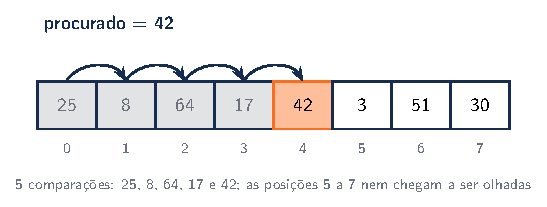
\includegraphics[width=0.8\linewidth,keepaspectratio]{imagens/capitulo-07_sequencial.pdf}
\end{center}

Sua grande vantagem é não exigir nada dos dados: o vetor pode estar em qualquer ordem, e o tipo dos elementos só precisa saber se comparar com \texttt{==}. Com um \textit{template} (Capítulo 1), a mesma função serve para números, textos e qualquer outro tipo. E, quando os elementos são registros, a busca costuma ser feita por uma \textbf{chave}, um campo que identifica o registro, como a matrícula de um aluno:

\begin{codigo}
\begin{Verbatim}[breaklines=true, breaksymbolleft={}, fontsize=\footnotesize]
#include <vector>

template <typename T>
int buscaSequencial(const vector<T> &v, const T &procurado) {
    for (int i = 0; i < static_cast<int>(v.size()); i++) {
        if (v[i] == procurado) return i;   // achou: para
    }
    return -1;                     // olhou todos e não achou
}

struct Aluno {
    int matricula;
    string nome;
};

// procura pela chave (a matrícula) e devolve o aluno inteiro
const Aluno *buscarAluno(const vector<Aluno> &turma,
                         int matricula) {
    for (const Aluno &a : turma) {
        if (a.matricula == matricula) return &a;
    }
    return nullptr;                // nenhum aluno com ela
}

int main() {
    vector<int> numeros = {25, 8, 64, 17, 42, 3, 51, 30};
    cout << buscaSequencial(numeros, 42) << endl;   // 4
    cout << buscaSequencial(numeros, 99) << endl;   // -1

    vector<string> cores = {"azul", "verde", "roxo"};
    cout << buscaSequencial(cores, string("roxo")) << endl; // 2

    vector<Aluno> turma = {{2031, "Ana"}, {1987, "Bruno"},
                           {2210, "Carla"}};
    const Aluno *achado = buscarAluno(turma, 1987);
    if (achado != nullptr) cout << achado->nome << endl; // Bruno
}
\end{Verbatim}
\end{codigo}

O \texttt{string("roxo")} é necessário porque \texttt{"roxo"} sozinho é um texto do C, e o \textit{template} precisa que os dois parâmetros sejam do mesmo tipo \texttt{T}. A função \texttt{buscarAluno} devolve um ponteiro para o aluno encontrado, ou \texttt{nullptr} quando não acha, o mesmo papel do $-1$ na versão com índices.

Como você viu no Capítulo 2, o melhor caso é uma comparação, o pior caso são $n$ comparações (o valor está no fim ou não existe) e o caso médio é cerca de $n/2$. A busca sequencial é $O(n)$.

\subsubsection{Duas melhorias simples}

Se o vetor estiver \textbf{ordenado}, a busca pode desistir mais cedo: ao encontrar um valor maior que o procurado, já se sabe que ele não está no resto do vetor. Isso não muda o pior caso, que continua $O(n)$, mas acelera as buscas sem sucesso.

A outra melhoria é a \textbf{sentinela}. O laço da busca sequencial faz duas perguntas a cada passo: ``o vetor acabou?'' e ``achei?''. Se o próprio valor procurado for colocado no fim do vetor, o laço com certeza vai parar nele, e a primeira pergunta deixa de ser necessária. No final, basta ver se o valor encontrado foi o verdadeiro ou a sentinela.

\begin{codigo}
\begin{Verbatim}[breaklines=true, breaksymbolleft={}, fontsize=\footnotesize]
#include <vector>

// vetor em ordem crescente: dá para desistir mais cedo
int buscaOrdenada(const vector<int> &v, int procurado) {
    for (int i = 0; i < static_cast<int>(v.size()); i++) {
        if (v[i] == procurado) return i;
        if (v[i] > procurado) return -1;   // o resto é maior
    }
    return -1;
}

// sentinela: uma comparação por passo em vez de duas
int buscaComSentinela(vector<int> &v, int procurado) {
    int n = static_cast<int>(v.size());
    v.push_back(procurado);       // garante que o laço para
    int i = 0;
    while (v[i] != procurado) i++;
    v.pop_back();                 // devolve o vetor como estava
    return i < n ? i : -1;        // parou na sentinela: não está
}
\end{Verbatim}
\end{codigo}

A sentinela economiza uma comparação por passo, o que pode fazer diferença em laços executados milhões de vezes, mas continua $O(n)$. Ela é um exemplo de otimização que melhora a constante, e não a ordem de crescimento.

\subsection{7.2 Busca binária}

Pense no jogo de adivinhar um número de 1 a 100, em que a cada palpite você ouve ``é maior'' ou ``é menor''. Ninguém joga chutando 1, 2, 3\ldots{} A estratégia natural é chutar 50: seja qual for a resposta, metade das possibilidades desaparece. Depois 25 ou 75, e assim por diante. Em no máximo 7 palpites você acerta.

A \textbf{busca binária} usa exatamente essa ideia em um vetor \textbf{ordenado}. Ela mantém uma faixa de posições onde o valor ainda pode estar, delimitada por \texttt{inicio} e \texttt{fim}, e a cada passo compara o procurado com o elemento do \textbf{meio} da faixa:

\begin{itemize}
  \item se for igual, achou;
  \item se o elemento do meio for \textbf{menor} que o procurado, o valor só pode estar à direita, e a faixa passa a começar em \texttt{meio + 1};
  \item se for \textbf{maior}, o valor só pode estar à esquerda, e a faixa passa a terminar em \texttt{meio - 1};
  \item se a faixa ficar vazia (\texttt{inicio > fim}), o valor não está no vetor.
\end{itemize}

\begin{center}
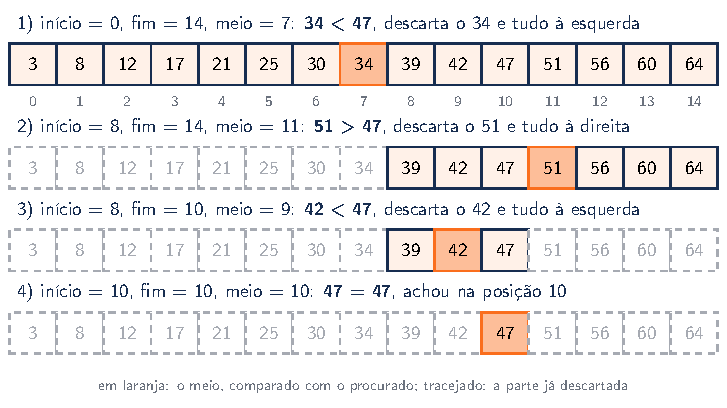
\includegraphics[width=\linewidth,keepaspectratio]{imagens/capitulo-07_binaria.pdf}
\end{center}

\begin{codigo}
\begin{Verbatim}[breaklines=true, breaksymbolleft={}, fontsize=\footnotesize]
// trecho
int buscaBinaria(const vector<int> &v, int procurado) {
    int inicio = 0;
    int fim = static_cast<int>(v.size()) - 1;
    while (inicio <= fim) {           // ainda há onde procurar
        int meio = inicio + (fim - inicio) / 2;
        if (v[meio] == procurado) return meio;
        if (v[meio] < procurado) {
            inicio = meio + 1;        // descarta a esquerda
        } else {
            fim = meio - 1;           // descarta a direita
        }
    }
    return -1;                        // a faixa ficou vazia
}
\end{Verbatim}
\end{codigo}

Acompanhar a busca em uma tabela, com os valores de cada variável a cada volta do laço, é a melhor forma de entendê-la. Veja o que acontece ao procurar o 20, que não está no vetor da figura:

\begin{center}
\begin{tabular}{@{}p{0.08\linewidth}p{0.1\linewidth}p{0.06\linewidth}p{0.08\linewidth}p{0.12\linewidth}p{0.32\linewidth}@{}}
\toprule
\rowcolor{headergray}
\tblheader{Passo} & \tblheader{início} & \tblheader{fim} & \tblheader{meio} & \tblheader{v[meio]} & \tblheader{Decisão} \\
\midrule
1 & 0 & 14 & 7 & 34 & 20 < 34: fim = 6 \\
\rowcolor{rowgray} 2 & 0 & 6 & 3 & 17 & 20 > 17: início = 4 \\
3 & 4 & 6 & 5 & 25 & 20 < 25: fim = 4 \\
\rowcolor{rowgray} 4 & 4 & 4 & 4 & 21 & 20 < 21: fim = 3 \\
-- & 4 & 3 & & & início > fim: não está \\
\bottomrule
\end{tabular}
\end{center}

Repare no valor final de \texttt{inicio}: 4, exatamente a posição em que o 20 deveria ser inserido para o vetor continuar ordenado, entre o 17 e o 21. Essa observação será útil na Seção 7.3.

\begin{destaque}{Por que não \texttt{(inicio + fim) / 2}?}
As duas fórmulas dão o mesmo meio, mas \texttt{inicio + fim} pode passar do maior valor que um \texttt{int} guarda (cerca de 2,1 bilhões) em vetores muito grandes, e o resultado vira um número negativo. Já \texttt{inicio + (fim - inicio) / 2} nunca passa de \texttt{fim}. Esse erro ficou escondido por anos na busca binária da biblioteca do Java, até ser descoberto em 2006, quando os vetores ficaram grandes o bastante para ele aparecer.
\end{destaque}

\subsubsection{Versão recursiva}

A busca binária também tem uma definição recursiva natural, como os percursos de árvore do Capítulo 5: o caso base é a faixa vazia, e cada chamada procura em uma das metades.

\begin{codigo}
\begin{Verbatim}[breaklines=true, breaksymbolleft={}, fontsize=\footnotesize]
// trecho
int buscaBinariaRecursiva(const vector<int> &v, int procurado,
                          int inicio, int fim) {
    if (inicio > fim) return -1;      // caso base: faixa vazia
    int meio = inicio + (fim - inicio) / 2;
    if (v[meio] == procurado) return meio;
    if (v[meio] < procurado) {
        return buscaBinariaRecursiva(v, procurado, meio + 1, fim);
    }
    return buscaBinariaRecursiva(v, procurado, inicio, meio - 1);
}
\end{Verbatim}
\end{codigo}

As duas versões fazem as mesmas comparações. A iterativa é a mais usada na prática, porque não gasta a pilha de execução; a recursiva é mais próxima da definição e aparece muito em provas. Este é o programa completo com as duas:

\begin{codigo}
\begin{Verbatim}[breaklines=true, breaksymbolleft={}, fontsize=\footnotesize]
#include <vector>

int buscaBinaria(const vector<int> &v, int procurado) {
    int inicio = 0;
    int fim = static_cast<int>(v.size()) - 1;
    while (inicio <= fim) {           // ainda há onde procurar
        int meio = inicio + (fim - inicio) / 2;
        if (v[meio] == procurado) return meio;
        if (v[meio] < procurado) {
            inicio = meio + 1;        // descarta a esquerda
        } else {
            fim = meio - 1;           // descarta a direita
        }
    }
    return -1;                        // a faixa ficou vazia
}

int buscaBinariaRecursiva(const vector<int> &v, int procurado,
                          int inicio, int fim) {
    if (inicio > fim) return -1;      // caso base: faixa vazia
    int meio = inicio + (fim - inicio) / 2;
    if (v[meio] == procurado) return meio;
    if (v[meio] < procurado) {
        return buscaBinariaRecursiva(v, procurado, meio + 1, fim);
    }
    return buscaBinariaRecursiva(v, procurado, inicio, meio - 1);
}

int main() {
    vector<int> v = {3, 8, 12, 17, 21, 25, 30, 34, 39, 42,
                     47, 51, 56, 60, 64};
    cout << buscaBinaria(v, 47) << endl;            // 10
    cout << buscaBinaria(v, 20) << endl;            // -1
    cout << buscaBinaria(v, 3) << " "
         << buscaBinaria(v, 64) << endl;            // 0 14
    int ultimo = static_cast<int>(v.size()) - 1;
    cout << buscaBinariaRecursiva(v, 47, 0, ultimo) << endl; // 10
}
\end{Verbatim}
\end{codigo}

\subsubsection{Quanto custa}

Cada comparação descarta metade da faixa: de $n$ posições sobram $n/2$, depois $n/4$, $n/8$\ldots{} até sobrar uma. O número de passos é quantas vezes $n$ pode ser dividido por 2, ou seja, $\log_2 n$. A busca binária é $O(\log n)$, e é isso que a torna tão poderosa:

\begin{center}
\begin{tabular}{@{}p{0.3\linewidth}p{0.32\linewidth}p{0.28\linewidth}@{}}
\toprule
\rowcolor{headergray}
\tblheader{Tamanho do vetor} & \tblheader{Sequencial (pior caso)} & \tblheader{Binária (pior caso)} \\
\midrule
15 & 15 comparações & 4 comparações \\
\rowcolor{rowgray} 1.000 & 1.000 & 10 \\
1.000.000 & 1.000.000 & 20 \\
\rowcolor{rowgray} 1.000.000.000 & 1.000.000.000 & 30 \\
\bottomrule
\end{tabular}
\end{center}

Multiplicar o vetor por mil acrescenta só 10 comparações. Mas a busca binária cobra um preço: o vetor precisa estar \textbf{ordenado}, e precisa permitir acesso direto a qualquer posição. Em uma lista encadeada (Capítulo 3), chegar ao meio já custa $O(n)$, e a vantagem desaparece.

\subsection{7.3 Variações da busca binária}

A busca binária básica responde ``está ou não está?''. Com pequenas mudanças, ela responde perguntas mais úteis.

\subsubsection{Primeira ocorrência e ponto de inserção}

Quando o vetor tem valores repetidos, a busca básica devolve a posição de \textbf{algum} deles, não necessariamente a do primeiro. A variação abaixo encontra a \textbf{primeira posição com valor maior ou igual} ao procurado. Se o valor existe, é a sua primeira ocorrência; se não existe, é a posição onde ele deveria ser inserido.

A diferença está no tratamento do meio: quando \texttt{v[meio]} é maior ou igual ao procurado, o meio ainda pode ser a resposta, então a faixa passa a terminar \textbf{nele} (\texttt{fim = meio}), em vez de descartá-lo. Para isso funcionar, \texttt{fim} começa fora do vetor, em \texttt{v.size()}, e o laço para quando \texttt{inicio} e \texttt{fim} se encontram.

Com ela, contar quantas vezes um valor aparece também fica $O(\log n)$: é a distância entre a primeira posição do valor e a primeira posição do valor seguinte.

\subsubsection{Busca binária na resposta}

A busca binária não precisa de um vetor. Ela funciona em qualquer faixa de números em que uma pergunta tenha resposta ``sim'' até certo ponto e ``não'' daí em diante. Um exemplo é a raiz quadrada inteira de $n$: o maior $x$ tal que $x^2 \le n$. Para $x = 0, 1, 2, \ldots$, a resposta a ``$x^2 \le n$?'' é sim, sim, sim\ldots{} e depois sempre não. A busca binária encontra o último ``sim'' sem testar um por um.

\begin{codigo}
\begin{Verbatim}[breaklines=true, breaksymbolleft={}, fontsize=\footnotesize]
#include <vector>

// primeira posição com valor >= procurado
// (v.size() se todos forem menores)
int primeiraPosicao(const vector<int> &v, int procurado) {
    int inicio = 0;
    int fim = static_cast<int>(v.size());  // fora do vetor
    while (inicio < fim) {
        int meio = inicio + (fim - inicio) / 2;
        if (v[meio] < procurado) {
            inicio = meio + 1;     // a resposta está à direita
        } else {
            fim = meio;            // o meio ainda pode ser ela
        }
    }
    return inicio;
}

int contar(const vector<int> &v, int valor) {
    return primeiraPosicao(v, valor + 1)
           - primeiraPosicao(v, valor);
}

// maior x tal que x * x <= n
long long raizInteira(long long n) {
    long long inicio = 1, fim = n, resposta = 0;
    while (inicio <= fim) {
        long long meio = inicio + (fim - inicio) / 2;
        if (meio <= n / meio) {    // meio * meio <= n sem estouro
            resposta = meio;       // serve; tenta um maior
            inicio = meio + 1;
        } else {
            fim = meio - 1;        // grande demais
        }
    }
    return resposta;
}

int main() {
    vector<int> notas = {4, 5, 5, 7, 7, 7, 8, 9, 10};
    cout << primeiraPosicao(notas, 7) << endl;  // 3: 1º 7
    cout << primeiraPosicao(notas, 6) << endl;  // 3: entraria
    cout << primeiraPosicao(notas, 11) << endl; // 9: no fim
    cout << contar(notas, 7) << " "
         << contar(notas, 6) << endl;            // 3 0

    cout << raizInteira(50) << " "
         << raizInteira(1000000) << endl;        // 7 1000
    cout << raizInteira(1000000000000) << endl;  // 1000000
}
\end{Verbatim}
\end{codigo}

Na \texttt{raizInteira}, a comparação \texttt{meio <= n / meio} evita calcular \texttt{meio * meio}, que estouraria até um \texttt{long long} com $n$ na casa do trilhão. A mesma técnica resolve problemas como ``qual o menor tamanho de página que faz o texto caber em 10 páginas?'' ou ``qual a menor velocidade que permite terminar a entrega a tempo?'': sempre que a resposta pode ser testada e o teste muda de ``não'' para ``sim'' uma única vez.

\subsection{7.4 Busca na biblioteca padrão}

Na prática, você raramente vai escrever essas buscas do zero: o C++ traz todas elas prontas na biblioteca \texttt{<algorithm>}. Elas trabalham com \textbf{iteradores}, que indicam posições: \texttt{v.begin()} é o início do vetor e \texttt{v.end()} é a posição logo depois do último. Subtrair \texttt{v.begin()} de um iterador dá o índice.

\begin{codigo}
\begin{Verbatim}[breaklines=true, breaksymbolleft={}, fontsize=\footnotesize]
#include <vector>
#include <algorithm>   // find, sort, lower_bound...

int main() {
    vector<int> v = {25, 8, 64, 17, 42, 3, 51, 30};
    auto it = find(v.begin(), v.end(), 42);    // sequencial: O(n)
    if (it != v.end()) {
        cout << "posição " << it - v.begin() << endl; // 4
    }

    sort(v.begin(), v.end());           // 3 8 17 25 30 42 51 64
    cout << boolalpha
         << binary_search(v.begin(), v.end(), 42) << endl; // true

    auto p = lower_bound(v.begin(), v.end(), 20);  // 1º >= 20
    cout << *p << " na posição " << p - v.begin() << endl;
    // 25 na posição 3

    vector<int> notas = {4, 5, 5, 7, 7, 7, 8, 9, 10};
    auto [primeiro, depois] =
        equal_range(notas.begin(), notas.end(), 7);
    cout << depois - primeiro << " notas 7" << endl;  // 3 notas 7
}
\end{Verbatim}
\end{codigo}

\begin{center}
\begin{tabular}{@{}p{0.25\linewidth}p{0.17\linewidth}p{0.5\linewidth}@{}}
\toprule
\rowcolor{headergray}
\tblheader{Função} & \tblheader{Custo} & \tblheader{Devolve} \\
\midrule
\texttt{find} & $O(n)$ & iterador para o elemento, ou \texttt{end()} se não achar \\
\rowcolor{rowgray} \texttt{binary\_search} & $O(\log n)$ & \texttt{true} ou \texttt{false} \\
\texttt{lower\_bound} & $O(\log n)$ & primeira posição com valor $\ge$ procurado \\
\rowcolor{rowgray} \texttt{upper\_bound} & $O(\log n)$ & primeira posição com valor $>$ procurado \\
\texttt{equal\_range} & $O(\log n)$ & o par (\texttt{lower\_bound}, \texttt{upper\_bound}) \\
\bottomrule
\end{tabular}
\end{center}

A \texttt{lower\_bound} é a \texttt{primeiraPosicao} da Seção 7.3. Todas as funções de busca binária supõem que o vetor já está ordenado; se não estiver, elas não acusam erro nenhum, apenas devolvem respostas erradas. A \texttt{sort} usada no exemplo ordena o vetor em $O(n \log n)$; o Capítulo 8 mostra como algoritmos assim funcionam por dentro.

\subsection{7.5 Qual busca usar}

Se a busca binária é tão mais rápida, por que não usá-la sempre? Porque ordenar também custa. Ordenar um vetor de um milhão de elementos custa algo como $n \log_2 n \approx 20$ milhões de operações, muito mais que uma única busca sequencial (um milhão). A conta muda quando o mesmo vetor é consultado muitas vezes:

\begin{center}
\begin{tabular}{@{}p{0.2\linewidth}p{0.32\linewidth}p{0.4\linewidth}@{}}
\toprule
\rowcolor{headergray}
\tblheader{Buscas} & \tblheader{Só sequencial} & \tblheader{Ordenar uma vez + binária} \\
\midrule
1 & 1 milhão & 20 milhões + 20 \\
\rowcolor{rowgray} 100 & 100 milhões & 20 milhões + 2 mil \\
1 milhão & 1 trilhão & 20 milhões + 20 milhões \\
\bottomrule
\end{tabular}
\end{center}

Para uma busca isolada, a sequencial ganha; a partir de umas poucas dezenas de buscas no mesmo vetor, ordenar compensa com folga. A escolha também depende de quanto os dados mudam. Manter um vetor ordenado custa caro: cada inserção precisa deslocar os elementos maiores para abrir espaço. Por isso existem estruturas feitas para buscar e inserir rápido ao mesmo tempo:

\begin{center}
\begin{tabular}{@{}p{0.42\linewidth}p{0.24\linewidth}p{0.26\linewidth}@{}}
\toprule
\rowcolor{headergray}
\tblheader{Estrutura} & \tblheader{Buscar} & \tblheader{Inserir} \\
\midrule
vetor fora de ordem & $O(n)$ & $O(1)$ no fim \\
\rowcolor{rowgray} vetor ordenado & $O(\log n)$ & $O(n)$ \\
lista encadeada (Capítulo 3) & $O(n)$ & $O(1)$ no início \\
\rowcolor{rowgray} árvore AVL (Capítulo 5) & $O(\log n)$ & $O(\log n)$ \\
tabela hash (\texttt{unordered\_map}) & $O(1)$ em média & $O(1)$ em média \\
\bottomrule
\end{tabular}
\end{center}

Resumindo: poucos dados ou uma busca só, use a sequencial; dados que mudam pouco e são muito consultados, ordene e use a binária; dados que mudam e são consultados o tempo todo, use uma árvore balanceada (o \texttt{set} e o \texttt{map} do C++) ou uma tabela hash (o \texttt{unordered\_set} e o \texttt{unordered\_map}), que encontra uma chave em tempo médio constante calculando, a partir da própria chave, a posição onde ela está guardada.

\begin{destaque}{Comparando com Python}
Em Python, o operador \texttt{in} e o método \texttt{index} das listas fazem busca sequencial, $O(n)$. A busca binária está no módulo \texttt{bisect}: \texttt{bisect\_left} é a \texttt{lower\_bound} do C++ e \texttt{bisect\_right} é a \texttt{upper\_bound}.

\begin{codigo}
\begin{Verbatim}[breaklines=true, breaksymbolleft={}, fontsize=\footnotesize]
from bisect import bisect_left, bisect_right

numeros = [3, 8, 12, 17, 21, 25, 30, 34, 39, 42,
           47, 51, 56, 60, 64]
print(42 in numeros)        # True: busca sequencial
print(numeros.index(42))    # 9

def busca_binaria(v, procurado):
    inicio, fim = 0, len(v) - 1
    while inicio <= fim:
        meio = (inicio + fim) // 2
        if v[meio] == procurado:
            return meio
        if v[meio] < procurado:
            inicio = meio + 1
        else:
            fim = meio - 1
    return -1

print(busca_binaria(numeros, 47))   # 10

notas = [4, 5, 5, 7, 7, 7, 8, 9, 10]
print(bisect_left(notas, 7))                            # 3
print(bisect_right(notas, 7) - bisect_left(notas, 7))   # 3
\end{Verbatim}
\end{codigo}

Como os inteiros do Python não têm limite, \texttt{(inicio + fim) // 2} não estoura. Repare no \texttt{//}, a divisão inteira: com \texttt{/}, o resultado seria um \texttt{float} e não serviria de índice. Para buscar muitas vezes por chave, o Python usa o \texttt{set} e o \texttt{dict}, que são tabelas hash: \texttt{42 in conjunto} é $O(1)$ em média, enquanto \texttt{42 in lista} é $O(n)$.
\end{destaque}

\subsection{Erros Comuns}

\begin{itemize}
  \item \textbf{Usar a busca binária em um vetor fora de ordem.} Ela não acusa erro: simplesmente descarta a metade errada e responde que o valor não está lá, mesmo quando está.
  \item \textbf{Errar a condição do laço.} Com \texttt{inicio} e \texttt{fim} apontando para posições válidas, o laço é \texttt{while (inicio <= fim)}. Com \texttt{<}, a busca deixa de olhar a última posição que sobrou.
  \item \textbf{Não descartar o meio.} Escrever \texttt{inicio = meio} em vez de \texttt{inicio = meio + 1} pode fazer a faixa parar de diminuir, e o laço nunca termina.
  \item \textbf{Calcular o meio com \texttt{(inicio + fim) / 2}} em vetores enormes. A soma pode estourar o \texttt{int}; use \texttt{inicio + (fim - inicio) / 2}.
  \item \textbf{Esperar a primeira ocorrência da busca básica.} Com valores repetidos, ela devolve um deles, não necessariamente o primeiro. Para o primeiro, use a \texttt{lower\_bound}.
  \item \textbf{Usar a busca binária em uma lista encadeada.} Sem acesso direto às posições, chegar ao meio já custa $O(n)$.
  \item \textbf{Ordenar o vetor para fazer uma única busca.} A ordenação custa mais que a própria busca sequencial; só compensa quando o vetor é consultado muitas vezes.
  \item \textbf{Esquecer de conferir o resultado de \texttt{find} e \texttt{lower\_bound}.} Se o valor não existir, elas devolvem \texttt{end()}, e usar \texttt{*it} nesse caso acessa uma posição fora do vetor.
\end{itemize}

\newpage
\section{Capítulo 8 -- Ordenação}

No Capítulo 7 você viu que a busca binária encontra um valor entre um bilhão em 30 comparações, desde que o vetor esteja \textbf{ordenado}. Ordenar dados é uma das tarefas mais comuns da computação: listas de alunos em ordem alfabética, produtos do mais barato ao mais caro, mensagens da mais recente à mais antiga. Também é um dos melhores lugares para aprender a projetar algoritmos, porque o mesmo problema tem soluções muito diferentes. Neste capítulo você vai estudar seis delas: três simples, de custo $O(n^2)$, e três eficientes, de custo $O(n \log n)$. No caminho, vai construir o \textit{heap}, a estrutura que o Capítulo 6 usou dentro da fila de prioridade.

\subsection{8.1 O problema da ordenação}

Ordenar é rearranjar os elementos de um vetor para que fiquem em ordem crescente (ou decrescente) segundo algum critério. Todos os algoritmos deste capítulo são \textbf{baseados em comparações}: a única coisa que fazem com os elementos é perguntar ``este é menor que aquele?'' e trocá-los de lugar. Por isso, servem para qualquer tipo que saiba se comparar, de números a nomes e datas.

Além do tempo, três características ajudam a escolher um algoritmo:

\begin{itemize}
  \item \textbf{No lugar} (\textit{in-place}): o algoritmo usa apenas uma quantidade constante de memória extra, além do próprio vetor.
  \item \textbf{Estável}: elementos com a mesma chave continuam na ordem em que estavam. Se uma turma já está em ordem alfabética e você a ordena por nota com um algoritmo estável, os alunos com a mesma nota continuam em ordem alfabética.
  \item \textbf{Adaptativo}: o algoritmo trabalha menos quando o vetor já está quase ordenado.
\end{itemize}

Todos os exemplos usam o mesmo vetor de oito números, \texttt{\{29, 10, 14, 37, 13, 5, 41, 22\}}, e a função \texttt{swap} do C++, que troca o conteúdo de duas variáveis.

\subsection{8.2 Ordenação por bolha (\textit{bubble sort})}

A ordenação por bolha percorre o vetor comparando cada par de vizinhos e trocando os dois sempre que estiverem fora de ordem. Ao fim da primeira passada, o maior elemento foi empurrado, troca a troca, até a última posição, como uma bolha que sobe até a superfície. A segunda passada leva o segundo maior para a penúltima posição, e assim por diante.

\begin{center}
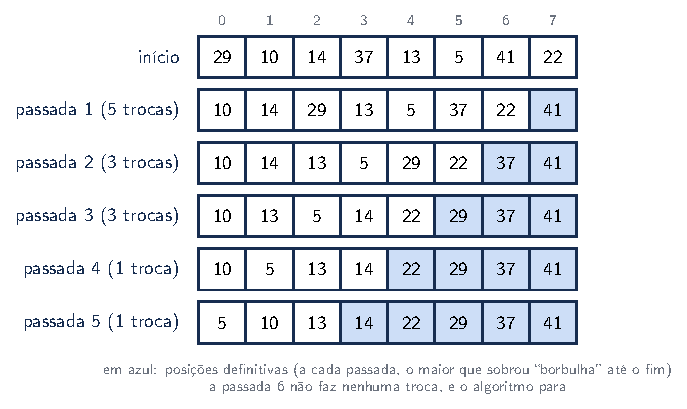
\includegraphics[width=0.85\linewidth,keepaspectratio]{imagens/capitulo-08_bolha.pdf}
\end{center}

\begin{codigo}
\begin{Verbatim}[breaklines=true, breaksymbolleft={}, fontsize=\footnotesize]
// trecho
void bolha(vector<int> &v) {
    int n = static_cast<int>(v.size());
    for (int passada = 0; passada < n - 1; passada++) {
        bool trocou = false;
        // os últimos "passada" elementos já estão no lugar
        for (int i = 0; i < n - 1 - passada; i++) {
            if (v[i] > v[i + 1]) {
                swap(v[i], v[i + 1]);
                trocou = true;
            }
        }
        if (!trocou) return;   // nenhuma troca: já está ordenado
    }
}
\end{Verbatim}
\end{codigo}

A variável \texttt{trocou} é o que torna a bolha adaptativa: se uma passada inteira não fizer nenhuma troca, o vetor já está ordenado e o algoritmo para. Em um vetor já ordenado, basta uma passada, $O(n)$. No pior caso, o vetor em ordem inversa, são $n - 1$ passadas com cerca de $n^2/2$ comparações e trocas: $O(n^2)$. A bolha é estável, porque só troca vizinhos estritamente fora de ordem, e funciona no lugar.

\subsection{8.3 Ordenação por seleção (\textit{selection sort})}

A ordenação por seleção faz o que muita gente faria à mão: procura o menor elemento e o coloca na primeira posição; depois procura o menor entre os que sobraram e o coloca na segunda, e assim por diante.

\begin{codigo}
\begin{Verbatim}[breaklines=true, breaksymbolleft={}, fontsize=\footnotesize]
// trecho
void selecao(vector<int> &v) {
    int n = static_cast<int>(v.size());
    for (int i = 0; i < n - 1; i++) {
        int menor = i;
        for (int j = i + 1; j < n; j++) {  // o menor do resto
            if (v[j] < v[menor]) menor = j;
        }
        swap(v[i], v[menor]);              // uma troca só
    }
}
\end{Verbatim}
\end{codigo}

A seleção sempre faz cerca de $n^2/2$ comparações, mesmo que o vetor já esteja ordenado: ela não é adaptativa, e é $O(n^2)$ em todos os casos. Sua vantagem é fazer no máximo $n - 1$ trocas, o que importa quando mover um elemento custa muito mais que compará-lo. Ela não é estável: a troca pode levar um elemento para depois de outro igual a ele.

\subsection{8.4 Ordenação por inserção (\textit{insertion sort})}

A ordenação por inserção é o jeito como se arruma uma mão de cartas: as cartas da esquerda já estão em ordem, e cada nova carta é encaixada no lugar certo entre elas. No vetor, a parte ordenada começa com um único elemento e cresce uma posição a cada passo. Para abrir espaço para o novo elemento, os maiores que ele são deslocados uma posição para a direita.

\begin{center}
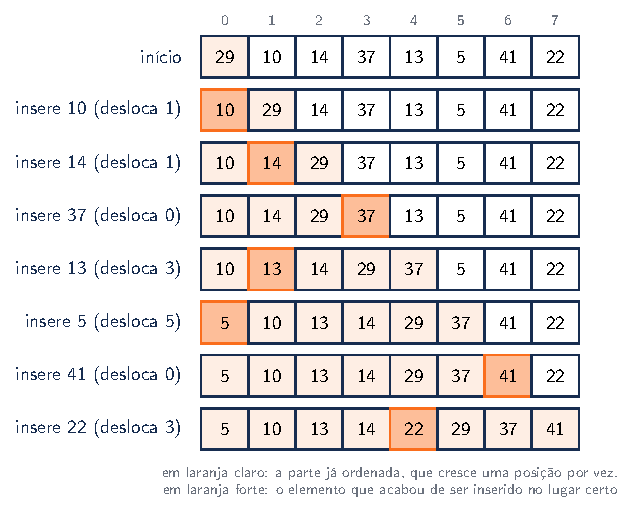
\includegraphics[width=0.85\linewidth,keepaspectratio]{imagens/capitulo-08_insercao.pdf}
\end{center}

\begin{codigo}
\begin{Verbatim}[breaklines=true, breaksymbolleft={}, fontsize=\footnotesize]
// trecho
void insercao(vector<int> &v) {
    int n = static_cast<int>(v.size());
    for (int i = 1; i < n; i++) {
        int chave = v[i];        // o próximo a ser inserido
        int j = i - 1;
        while (j >= 0 && v[j] > chave) {
            v[j + 1] = v[j];     // desloca o maior à direita
            j--;
        }
        v[j + 1] = chave;        // encaixa no espaço aberto
    }
}
\end{Verbatim}
\end{codigo}

O laço \texttt{while} para assim que encontra um elemento menor ou igual à chave. Em um vetor já ordenado, ele para logo na primeira comparação, e a inserção inteira custa $O(n)$; em um vetor quase ordenado, faz poucos deslocamentos. No pior caso, em ordem inversa, cada elemento percorre toda a parte ordenada: $O(n^2)$. A inserção é estável, porque o \texttt{>} nunca passa uma chave para antes de outra igual, e funciona no lugar.

O programa completo ordena o vetor de exemplo com os três algoritmos:

\begin{codigo}
\begin{Verbatim}[breaklines=true, breaksymbolleft={}, fontsize=\footnotesize]
#include <vector>
#include <utility>   // swap

void bolha(vector<int> &v) {
    int n = static_cast<int>(v.size());
    for (int passada = 0; passada < n - 1; passada++) {
        bool trocou = false;
        for (int i = 0; i < n - 1 - passada; i++) {
            if (v[i] > v[i + 1]) {
                swap(v[i], v[i + 1]);
                trocou = true;
            }
        }
        if (!trocou) return;
    }
}

void selecao(vector<int> &v) {
    int n = static_cast<int>(v.size());
    for (int i = 0; i < n - 1; i++) {
        int menor = i;
        for (int j = i + 1; j < n; j++) {
            if (v[j] < v[menor]) menor = j;
        }
        swap(v[i], v[menor]);
    }
}

void insercao(vector<int> &v) {
    int n = static_cast<int>(v.size());
    for (int i = 1; i < n; i++) {
        int chave = v[i];
        int j = i - 1;
        while (j >= 0 && v[j] > chave) {
            v[j + 1] = v[j];
            j--;
        }
        v[j + 1] = chave;
    }
}

void mostrar(const vector<int> &v) {
    for (int x : v) cout << x << " ";
    cout << endl;
}

int main() {
    const vector<int> exemplo = {29, 10, 14, 37, 13, 5, 41, 22};
    vector<int> a = exemplo, b = exemplo, c = exemplo;
    bolha(a);
    selecao(b);
    insercao(c);
    mostrar(a);   // 5 10 13 14 22 29 37 41
    mostrar(b);   // 5 10 13 14 22 29 37 41
    mostrar(c);   // 5 10 13 14 22 29 37 41
}
\end{Verbatim}
\end{codigo}

Os três são $O(n^2)$ no pior caso, mas se comportam de forma bem diferente conforme a entrada. Esta tabela mostra quantas comparações e quantas trocas (ou deslocamentos, na inserção) cada um faz em um vetor de 1.000 elementos, no formato ``comparações / trocas'':

\begin{center}
\begin{tabular}{@{}p{0.24\linewidth}p{0.3\linewidth}p{0.32\linewidth}@{}}
\toprule
\rowcolor{headergray}
\tblheader{Algoritmo} & \tblheader{Já ordenado} & \tblheader{Em ordem inversa} \\
\midrule
bolha & 999 / 0 & 499.500 / 499.500 \\
\rowcolor{rowgray} seleção & 499.500 / 999 & 499.500 / 999 \\
inserção & 999 / 0 & 499.500 / 499.500 \\
\bottomrule
\end{tabular}
\end{center}

Na prática, a inserção é a melhor dos três: é simples, estável, adaptativa e muito rápida em vetores pequenos ou quase ordenados. Por isso, ela aparece dentro dos algoritmos de ordenação das bibliotecas, como você verá na Seção 8.8.

\subsection{8.5 Ordenação por intercalação (\textit{merge sort})}

Para fugir do $O(n^2)$, é preciso parar de comparar quase todos os pares. A ordenação por intercalação usa a estratégia \textbf{dividir para conquistar}, a mesma ideia de reduzir um problema a problemas menores que você viu na recursão:

\begin{enumerate}
  \item \textbf{Dividir}: separe o vetor em duas metades.
  \item \textbf{Conquistar}: ordene cada metade, recursivamente. Um vetor com zero ou um elemento já está ordenado.
  \item \textbf{Combinar}: \textbf{intercale} as duas metades ordenadas em um único vetor ordenado.
\end{enumerate}

\begin{center}
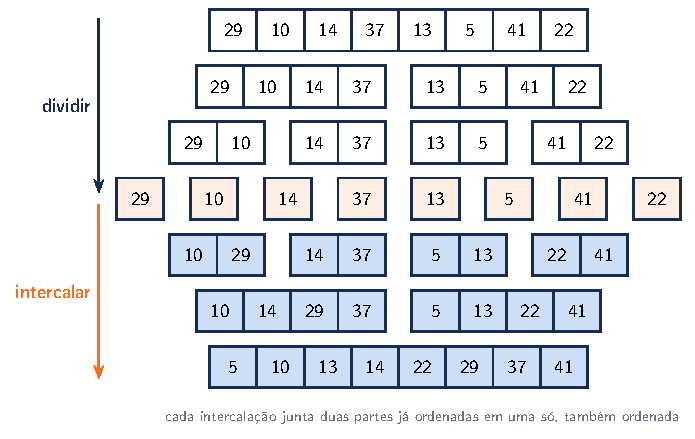
\includegraphics[width=0.85\linewidth,keepaspectratio]{imagens/capitulo-08_intercalacao.pdf}
\end{center}

Todo o trabalho está na intercalação. Como as duas metades já estão ordenadas, o menor de todos só pode ser o primeiro de uma delas. Basta comparar os primeiros de cada metade, copiar o menor para um vetor auxiliar e avançar naquela metade, até uma delas acabar; o que sobrar da outra já está em ordem e é copiado no fim.

\begin{codigo}
\begin{Verbatim}[breaklines=true, breaksymbolleft={}, fontsize=\footnotesize]
// trecho
// junta v[ini..meio] e v[meio+1..fim], já ordenados, em um só
void intercalar(vector<int> &v, int ini, int meio, int fim) {
    vector<int> aux;
    aux.reserve(fim - ini + 1);
    int i = ini, j = meio + 1;
    while (i <= meio && j <= fim) {
        if (v[i] <= v[j]) {      // empate: a esquerda primeiro
            aux.push_back(v[i++]);
        } else {
            aux.push_back(v[j++]);
        }
    }
    while (i <= meio) aux.push_back(v[i++]);  // sobras: esquerda
    while (j <= fim) aux.push_back(v[j++]);   // sobras: direita
    for (int k = 0; k < static_cast<int>(aux.size()); k++) {
        v[ini + k] = aux[k];                  // copia de volta
    }
}

void mergeSort(vector<int> &v, int ini, int fim) {
    if (ini >= fim) return;      // 0 ou 1 elemento: já ordenado
    int meio = ini + (fim - ini) / 2;
    mergeSort(v, ini, meio);
    mergeSort(v, meio + 1, fim);
    intercalar(v, ini, meio, fim);
}
\end{Verbatim}
\end{codigo}

O \texttt{v[i++]} usa o valor de \texttt{v[i]} e só depois avança o \texttt{i}. O \texttt{<=} na comparação faz o \textit{merge sort} ser estável: em caso de empate, o elemento da metade esquerda, que vinha antes, é copiado primeiro.

Para calcular o custo, olhe a figura por níveis. Intercalar todos os pedaços de um mesmo nível custa $O(n)$, porque cada elemento é copiado uma vez. E, como o vetor é dividido ao meio a cada nível, existem $\log_2 n$ níveis (3, para 8 elementos). O total é $O(n \log n)$, \textbf{em qualquer caso}: o \textit{merge sort} não depende da ordem da entrada. O preço é a memória: o vetor auxiliar ocupa $O(n)$, então ele não funciona no lugar.

\subsection{8.6 Ordenação rápida (\textit{quicksort})}

O \textit{quicksort} também divide para conquistar, mas faz o trabalho pesado \textbf{antes} da recursão, e não depois. Ele escolhe um elemento, o \textbf{pivô}, e \textbf{particiona} o vetor: os menores que o pivô vão para a esquerda, os maiores para a direita, e o pivô fica entre os dois grupos, que é exatamente a sua posição final. Depois, basta ordenar cada grupo recursivamente. Não há nada para combinar.

\begin{center}
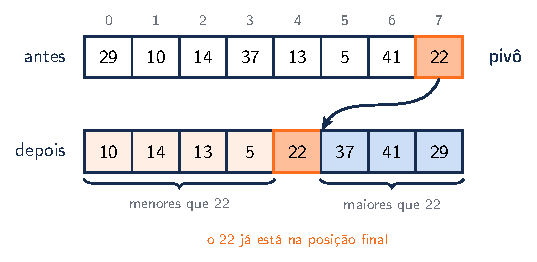
\includegraphics[width=0.75\linewidth,keepaspectratio]{imagens/capitulo-08_particao.pdf}
\end{center}

A partição abaixo usa o último elemento como pivô. A variável \texttt{i} marca o fim da região dos menores; cada elemento menor que o pivô encontrado por \texttt{j} é trocado para dentro dessa região, que cresce uma posição. No final, o pivô é trocado para logo depois dela.

\begin{codigo}
\begin{Verbatim}[breaklines=true, breaksymbolleft={}, fontsize=\footnotesize]
// trecho
// põe o pivô (o último) na posição final e devolve essa posição
int particionar(vector<int> &v, int ini, int fim) {
    int pivo = v[fim];
    int i = ini - 1;          // fim da região dos menores
    for (int j = ini; j < fim; j++) {
        if (v[j] < pivo) {
            i++;
            swap(v[i], v[j]); // entra na região dos menores
        }
    }
    swap(v[i + 1], v[fim]);   // pivô logo após os menores
    return i + 1;
}

void quickSort(vector<int> &v, int ini, int fim) {
    if (ini >= fim) return;
    int p = particionar(v, ini, fim);
    quickSort(v, ini, p - 1); // o pivô já está no lugar
    quickSort(v, p + 1, fim);
}
\end{Verbatim}
\end{codigo}

O custo depende de quão bem o pivô divide o vetor. Quando os dois grupos têm tamanhos parecidos, a recursão tem cerca de $\log_2 n$ níveis, cada um com $O(n)$ comparações, e o \textit{quicksort} é $O(n \log n)$. Na prática, ele costuma ser o mais rápido de todos, porque faz poucas trocas, não copia o vetor e percorre a memória em sequência.

\begin{destaque}{O pior caso do quicksort}
Se o pivô for sempre o maior ou o menor elemento, um dos grupos fica vazio e o outro tem $n - 1$ elementos. A recursão passa a ter $n$ níveis, e o custo vira $O(n^2)$. Com o último elemento como pivô, isso acontece justamente com um vetor \textbf{já ordenado}, uma entrada muito comum. Além de lento, o algoritmo pode estourar a pilha de execução com milhares de chamadas recursivas aninhadas. A solução é escolher melhor o pivô: o elemento do meio, um elemento sorteado ou a mediana entre o primeiro, o do meio e o último. Na partição acima, basta trocar o escolhido com o último antes de começar:

\begin{codigo}
\begin{Verbatim}[breaklines=true, breaksymbolleft={}, fontsize=\footnotesize]
// trecho
int meio = ini + (fim - ini) / 2;
swap(v[meio], v[fim]);   // o do meio passa a ser o pivô
\end{Verbatim}
\end{codigo}
\end{destaque}

O \textit{quicksort} funciona no lugar, usando só a pilha da recursão, $O(\log n)$ em média. Ele não é estável, porque as trocas da partição podem levar um elemento para longe, passando por cima de outros iguais a ele.

O programa completo testa os dois algoritmos no vetor de exemplo e em um vetor de 100 mil números pseudoaleatórios:

\begin{codigo}
\begin{Verbatim}[breaklines=true, breaksymbolleft={}, fontsize=\footnotesize]
#include <vector>
#include <utility>     // swap
#include <algorithm>   // is_sorted

void intercalar(vector<int> &v, int ini, int meio, int fim) {
    vector<int> aux;
    aux.reserve(fim - ini + 1);
    int i = ini, j = meio + 1;
    while (i <= meio && j <= fim) {
        if (v[i] <= v[j]) {
            aux.push_back(v[i++]);
        } else {
            aux.push_back(v[j++]);
        }
    }
    while (i <= meio) aux.push_back(v[i++]);
    while (j <= fim) aux.push_back(v[j++]);
    for (int k = 0; k < static_cast<int>(aux.size()); k++) {
        v[ini + k] = aux[k];
    }
}

void mergeSort(vector<int> &v, int ini, int fim) {
    if (ini >= fim) return;
    int meio = ini + (fim - ini) / 2;
    mergeSort(v, ini, meio);
    mergeSort(v, meio + 1, fim);
    intercalar(v, ini, meio, fim);
}

int particionar(vector<int> &v, int ini, int fim) {
    int meio = ini + (fim - ini) / 2;
    swap(v[meio], v[fim]);    // o do meio passa a ser o pivô
    int pivo = v[fim];
    int i = ini - 1;
    for (int j = ini; j < fim; j++) {
        if (v[j] < pivo) {
            i++;
            swap(v[i], v[j]);
        }
    }
    swap(v[i + 1], v[fim]);
    return i + 1;
}

void quickSort(vector<int> &v, int ini, int fim) {
    if (ini >= fim) return;
    int p = particionar(v, ini, fim);
    quickSort(v, ini, p - 1);
    quickSort(v, p + 1, fim);
}

int main() {
    vector<int> a = {29, 10, 14, 37, 13, 5, 41, 22};
    vector<int> b = a;
    mergeSort(a, 0, static_cast<int>(a.size()) - 1);
    quickSort(b, 0, static_cast<int>(b.size()) - 1);
    for (int x : a) cout << x << " ";
    cout << endl;             // 5 10 13 14 22 29 37 41

    vector<int> grande(100000);
    unsigned int semente = 42;
    for (int &x : grande) {   // gerador congruencial simples
        semente = semente * 1103515245u + 12345u;
        x = static_cast<int>(semente % 1000000);
    }
    vector<int> c = grande;
    int ultimo = static_cast<int>(grande.size()) - 1;
    mergeSort(grande, 0, ultimo);
    quickSort(c, 0, ultimo);
    cout << boolalpha << is_sorted(grande.begin(), grande.end())
         << " " << (grande == c) << endl;   // true true
}
\end{Verbatim}
\end{codigo}

A função \texttt{is\_sorted}, da biblioteca \texttt{<algorithm>}, confere se um vetor está em ordem, e \texttt{grande == c} compara os dois vetores posição por posição. Testar um algoritmo de ordenação com muitos dados gerados automaticamente encontra erros que um exemplo de oito números não mostraria; o Capítulo 11 volta a esse assunto.

\subsection{8.7 Heap e heapsort}

Um \textbf{heap} (máximo) é uma árvore binária com duas propriedades:

\begin{itemize}
  \item é \textbf{completa}: todos os níveis estão cheios, menos talvez o último, que é preenchido da esquerda para a direita;
  \item cada nó é \textbf{maior ou igual a seus filhos}. Por isso, o maior de todos está sempre na raiz.
\end{itemize}

Diferente da árvore binária de busca do Capítulo 5, o heap não diz nada sobre a ordem entre irmãos; ele só garante que cada pai vence os filhos. E, por ser completo, ele cabe em um vetor sem nenhum ponteiro: basta guardar os nós nível por nível, da esquerda para a direita.

\begin{center}
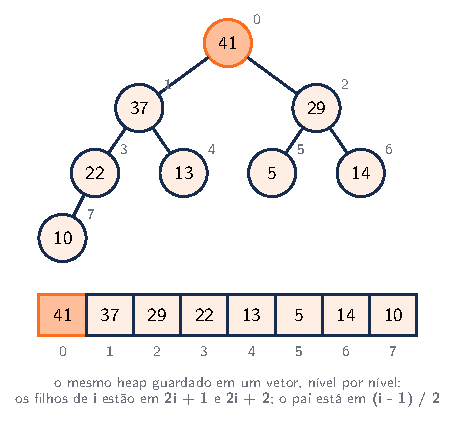
\includegraphics[width=0.65\linewidth,keepaspectratio]{imagens/capitulo-08_heap.pdf}
\end{center}

A operação central do heap é \textbf{descer}: quando um nó é menor que algum filho, ele troca de lugar com o maior dos filhos e continua descendo até ficar maior que os dois, ou chegar a uma folha. Como a altura de uma árvore completa é $\log_2 n$, descer custa $O(\log n)$.

O \textbf{heapsort} usa o heap em duas etapas:

\begin{enumerate}
  \item \textbf{Montar o heap}: faça descer cada nó que tem filhos, do último até a raiz. Ao final, o vetor de exemplo vira o heap da figura.
  \item \textbf{Ordenar}: o maior está na posição 0. Troque-o com o último elemento do heap, que passa a ter uma posição a menos, e faça a nova raiz descer para consertar o heap. Repita até sobrar um elemento. Os maiores vão sendo guardados no fim do vetor, do maior para o menor.
\end{enumerate}

\begin{codigo}
\begin{Verbatim}[breaklines=true, breaksymbolleft={}, fontsize=\footnotesize]
// trecho
// faz v[i] descer até o lugar certo em um heap de n elementos
void descer(vector<int> &v, int i, int n) {
    while (true) {
        int maior = i;
        int esq = 2 * i + 1, dir = 2 * i + 2;
        if (esq < n && v[esq] > v[maior]) maior = esq;
        if (dir < n && v[dir] > v[maior]) maior = dir;
        if (maior == i) return;   // já é maior que os filhos
        swap(v[i], v[maior]);
        i = maior;
    }
}

void heapSort(vector<int> &v) {
    int n = static_cast<int>(v.size());
    for (int i = n / 2 - 1; i >= 0; i--) {  // 1. monta o heap
        descer(v, i, n);
    }
    for (int fim = n - 1; fim > 0; fim--) { // 2. ordena
        swap(v[0], v[fim]);         // o maior vai para o fim
        descer(v, 0, fim);          // conserta o que sobrou
    }
}
\end{Verbatim}
\end{codigo}

Os nós com filhos são os de índice $0$ a $n/2 - 1$; os outros são folhas, que já são heaps de um elemento. Montar o heap custa $O(n)$ (a conta é mais sutil do que parece, porque a maioria dos nós está perto das folhas e desce pouco), e cada uma das $n - 1$ retiradas custa $O(\log n)$. O \textit{heapsort} é $O(n \log n)$ em \textbf{qualquer caso}, como o \textit{merge sort}, e funciona no lugar, como o \textit{quicksort}. Ele não é estável.

\subsubsection{A fila de prioridade}

O heap também é a estrutura por trás da \texttt{priority\_queue} usada pelo Dijkstra e pelo Prim no Capítulo 6. Retirar o maior é o mesmo movimento do \textit{heapsort}: o último elemento vai para a raiz e desce. Inserir é o movimento contrário: o novo elemento entra no fim do vetor e \textbf{sobe}, trocando de lugar com o pai enquanto for maior que ele. As duas operações custam $O(\log n)$.

\begin{codigo}
\begin{Verbatim}[breaklines=true, breaksymbolleft={}, fontsize=\footnotesize]
#include <vector>
#include <utility>   // swap

void descer(vector<int> &v, int i, int n) {
    while (true) {
        int maior = i;
        int esq = 2 * i + 1, dir = 2 * i + 2;
        if (esq < n && v[esq] > v[maior]) maior = esq;
        if (dir < n && v[dir] > v[maior]) maior = dir;
        if (maior == i) return;
        swap(v[i], v[maior]);
        i = maior;
    }
}

void heapSort(vector<int> &v) {
    int n = static_cast<int>(v.size());
    for (int i = n / 2 - 1; i >= 0; i--) {
        descer(v, i, n);
    }
    for (int fim = n - 1; fim > 0; fim--) {
        swap(v[0], v[fim]);
        descer(v, 0, fim);
    }
}

class FilaPrioridade {
private:
    vector<int> dados;   // um heap máximo

public:
    bool vazia() const { return dados.empty(); }

    void inserir(int valor) {
        dados.push_back(valor);          // entra no fim...
        int i = static_cast<int>(dados.size()) - 1;
        while (i > 0 && dados[(i - 1) / 2] < dados[i]) {
            swap(dados[i], dados[(i - 1) / 2]);  // ...e sobe
            i = (i - 1) / 2;
        }
    }

    int remover() {                      // tira o maior
        int maior = dados[0];
        dados[0] = dados.back();         // o último vai à raiz...
        dados.pop_back();
        int n = static_cast<int>(dados.size());
        descer(dados, 0, n);             // ...e desce
        return maior;
    }
};

int main() {
    vector<int> v = {29, 10, 14, 37, 13, 5, 41, 22};
    heapSort(v);
    for (int x : v) cout << x << " ";
    cout << endl;                // 5 10 13 14 22 29 37 41

    FilaPrioridade fila;
    for (int x : {29, 10, 14, 37, 13}) fila.inserir(x);
    while (!fila.vazia()) cout << fila.remover() << " ";
    cout << endl;                // 37 29 14 13 10
}
\end{Verbatim}
\end{codigo}

\subsection{8.8 Comparando os algoritmos}

\begin{center}
\begin{tabular}{@{}p{0.2\linewidth}p{0.17\linewidth}p{0.17\linewidth}p{0.14\linewidth}p{0.1\linewidth}@{}}
\toprule
\rowcolor{headergray}
\tblheader{Algoritmo} & \tblheader{Médio} & \tblheader{Pior} & \tblheader{Memória} & \tblheader{Estável} \\
\midrule
bolha & $O(n^2)$ & $O(n^2)$ & $O(1)$ & sim \\
\rowcolor{rowgray} seleção & $O(n^2)$ & $O(n^2)$ & $O(1)$ & não \\
inserção & $O(n^2)$ & $O(n^2)$ & $O(1)$ & sim \\
\rowcolor{rowgray} \textit{merge sort} & $O(n \log n)$ & $O(n \log n)$ & $O(n)$ & sim \\
\textit{quicksort} & $O(n \log n)$ & $O(n^2)$ & $O(\log n)$ & não \\
\rowcolor{rowgray} \textit{heapsort} & $O(n \log n)$ & $O(n \log n)$ & $O(1)$ & não \\
\bottomrule
\end{tabular}
\end{center}

Nenhum é o melhor em tudo. O \textit{merge sort} é previsível e estável, mas gasta memória; o \textit{quicksort} é o mais rápido na média, mas tem um pior caso ruim; o \textit{heapsort} garante $O(n \log n)$ no lugar, mas costuma ser mais lento que os outros dois na prática. E, em vetores pequenos, de algumas dezenas de elementos, a simples inserção vence todos eles, porque faz pouquíssimo trabalho por passo.

\begin{destaque}{Dá para ordenar mais rápido que $O(n \log n)$?}
Não, se o algoritmo só puder comparar elementos. Um vetor de $n$ elementos pode estar em $n!$ ordens diferentes, e cada comparação, com resposta ``sim'' ou ``não'', no máximo corta pela metade as ordens ainda possíveis. Para separar todas elas são necessárias pelo menos $\log_2 (n!)$ comparações, que é da ordem de $n \log n$: para 1.000 elementos, cerca de 8.500. Algoritmos que não comparam, como a ordenação por contagem (\textit{counting sort}), escapam desse limite, mas só funcionam para chaves especiais, como inteiros em uma faixa pequena.
\end{destaque}

\subsubsection{Ordenação na biblioteca padrão}

No dia a dia, use a \texttt{sort} da biblioteca \texttt{<algorithm>}. Ela é um \textbf{introsort}: começa como um \textit{quicksort}, passa para o \textit{heapsort} se a recursão ficar funda demais (fugindo do pior caso) e termina os pedaços pequenos com a inserção. Quando precisar de estabilidade, use a \texttt{stable\_sort}, que é um \textit{merge sort}.

As duas aceitam um terceiro parâmetro, o \textbf{critério de comparação}: uma função que recebe dois elementos e responde se o primeiro deve vir antes do segundo. Ele pode ser um objeto pronto, como \texttt{greater<>()} para a ordem decrescente, ou uma função anônima (\textit{lambda}), escrita ali mesmo, que você vai estudar no Capítulo 10.

\begin{codigo}
\begin{Verbatim}[breaklines=true, breaksymbolleft={}, fontsize=\footnotesize]
#include <vector>
#include <algorithm>    // sort, stable_sort
#include <functional>   // greater

struct Aluno {
    string nome;
    double nota;
};

int main() {
    vector<int> v = {29, 10, 14, 37, 13, 5, 41, 22};
    sort(v.begin(), v.end());                // crescente
    sort(v.begin(), v.end(), greater<>());   // decrescente
    for (int x : v) cout << x << " ";
    cout << endl;                // 41 37 29 22 14 13 10 5

    vector<Aluno> turma = {{"Davi", 7.5}, {"Ana", 9.0},
                           {"Caio", 7.5}, {"Bia", 9.0}};
    // maior nota primeiro; no empate, mantém a ordem original
    stable_sort(turma.begin(), turma.end(),
                [](const Aluno &a, const Aluno &b) {
                    return a.nota > b.nota;
                });
    for (const Aluno &a : turma) cout << a.nome << " ";
    cout << endl;                // Ana Bia Davi Caio
}
\end{Verbatim}
\end{codigo}

Repare no resultado: Ana e Bia têm 9,0 e aparecem na ordem em que estavam (Ana antes de Bia), e o mesmo acontece com Davi e Caio. Com a \texttt{sort}, que não é estável, a ordem dentro de cada empate poderia ser qualquer uma.

\begin{destaque}{Comparando com Python}
Em Python, \texttt{sorted(lista)} devolve uma nova lista ordenada e \texttt{lista.sort()} ordena a própria lista. Os dois usam o \textbf{Timsort}, uma combinação de \textit{merge sort} e inserção que aproveita os trechos já ordenados da entrada. Ele é estável e $O(n \log n)$. Em vez de um critério de comparação, o Python usa uma \textbf{chave}: o parâmetro \texttt{key} recebe uma função que diz por qual valor cada elemento deve ser ordenado.

\begin{codigo}
\begin{Verbatim}[breaklines=true, breaksymbolleft={}, fontsize=\footnotesize]
numeros = [29, 10, 14, 37, 13, 5, 41, 22]
print(sorted(numeros))          # nova lista, em ordem crescente
numeros.sort(reverse=True)      # ordena a própria lista
print(numeros)                  # [41, 37, 29, 22, 14, 13, 10, 5]

turma = [('Davi', 7.5), ('Ana', 9.0), ('Caio', 7.5), ('Bia', 9.0)]
por_nota = sorted(turma, key=lambda aluno: aluno[1], reverse=True)
print([nome for nome, _ in por_nota])
# ['Ana', 'Bia', 'Davi', 'Caio']

def merge_sort(v):
    if len(v) <= 1:
        return v
    meio = len(v) // 2
    esquerda, direita = merge_sort(v[:meio]), merge_sort(v[meio:])
    resultado = []
    i = j = 0
    while i < len(esquerda) and j < len(direita):
        if esquerda[i] <= direita[j]:
            resultado.append(esquerda[i])
            i += 1
        else:
            resultado.append(direita[j])
            j += 1
    return resultado + esquerda[i:] + direita[j:]

print(merge_sort([29, 10, 14, 37, 13, 5, 41, 22]))
\end{Verbatim}
\end{codigo}

O fatiamento (\texttt{v[:meio]}, \texttt{esquerda[i:]}) deixa o \textit{merge sort} em Python bem curto, mas cada fatia cria uma lista nova. O módulo \texttt{heapq}, visto no Capítulo 6, oferece as operações do heap prontas sobre uma lista comum.
\end{destaque}

\subsection{Erros Comuns}

\begin{itemize}
  \item \textbf{Passar do fim do vetor na bolha.} O laço interno compara \texttt{v[i]} com \texttt{v[i + 1]}, então \texttt{i} precisa parar em \texttt{n - 2}. Com \texttt{i < n}, a última comparação lê uma posição que não existe.
  \item \textbf{Inverter as condições do \texttt{while} da inserção.} Em \texttt{while (v[j] > chave \&\& j >= 0)}, o \texttt{v[-1]} é lido antes de o \texttt{j >= 0} ser testado. A ordem certa é \texttt{j >= 0 \&\& v[j] > chave}: o \texttt{\&\&} para na primeira condição falsa.
  \item \textbf{Esquecer as sobras na intercalação.} Quando uma metade acaba, os elementos restantes da outra precisam ser copiados; sem os dois \texttt{while} finais, eles se perdem.
  \item \textbf{Usar \texttt{<} em vez de \texttt{<=} na intercalação.} O vetor continua ordenado, mas o \textit{merge sort} deixa de ser estável.
  \item \textbf{Usar sempre o último elemento como pivô.} Com dados já ordenados, o \textit{quicksort} vira $O(n^2)$ e pode estourar a pilha.
  \item \textbf{Achar que $O(n^2)$ é sempre pior.} Para vetores pequenos ou quase ordenados, a inserção costuma ser mais rápida que os algoritmos $O(n \log n)$.
  \item \textbf{Usar \texttt{<=} no critério de comparação da \texttt{sort}.} O critério precisa responder \texttt{false} quando os dois elementos são iguais. Com \texttt{<=}, o comportamento é indefinido, e o programa pode até travar.
  \item \textbf{Ordenar uma cópia sem perceber.} Se a função de ordenação recebe o vetor por valor, como em \texttt{vector<int> v}, ela ordena uma cópia, e o original continua igual. Use referência: \texttt{vector<int> \&v}.
\end{itemize}

\newpage
\section{Capítulo 9 -- Algoritmos gulosos e programação dinâmica}

Muitos problemas pedem não uma resposta qualquer, mas a \textbf{melhor} resposta: o troco com menos moedas, o maior número de reuniões em uma sala, a rede de estradas mais barata, a mochila com o maior valor. Esses são os \textbf{problemas de otimização}. Testar todas as possibilidades quase sempre é inviável, porque elas crescem de forma exponencial. Neste capítulo você vai conhecer duas técnicas para resolvê-los de forma eficiente: os \textbf{algoritmos gulosos}, que tomam a melhor decisão do momento e nunca voltam atrás, e a \textbf{programação dinâmica}, que resolve cada subproblema uma única vez e guarda a resposta. No caminho, você vai ver o algoritmo de Kruskal, prometido no Capítulo 6.

\subsection{9.1 Algoritmos gulosos}

Um algoritmo \textbf{guloso} constrói a solução passo a passo e, a cada passo, faz a escolha que parece melhor \textbf{naquele momento}, sem pensar nas consequências e sem desfazer escolhas anteriores. Você já conhece três: o Dijkstra, que sempre trata o vértice mais próximo; o Prim, que sempre pega a aresta mais barata; e a ordenação por seleção, que sempre busca o menor elemento.

O exemplo mais familiar é o troco. Para dar 87 centavos com as moedas brasileiras (1 real, 50, 25, 10, 5 e 1 centavo), qualquer caixa faz assim: usa a maior moeda que ainda cabe, desconta, e repete. São 50 + 25 + 10 + 1 + 1, cinco moedas, e não há como usar menos.

\begin{codigo}
\begin{Verbatim}[breaklines=true, breaksymbolleft={}, fontsize=\footnotesize]
#include <vector>

// usa sempre a maior moeda que ainda cabe
// (as moedas precisam estar em ordem decrescente)
vector<int> trocoGuloso(const vector<int> &moedas, int valor) {
    vector<int> usadas;
    for (int m : moedas) {
        while (valor >= m) {
            usadas.push_back(m);
            valor -= m;
        }
    }
    return usadas;
}

void mostrar(const vector<int> &v) {
    for (int x : v) cout << x << " ";
    cout << endl;
}

int main() {
    mostrar(trocoGuloso({100, 50, 25, 10, 5, 1}, 87));
    // 50 25 10 1 1
    mostrar(trocoGuloso({4, 3, 1}, 6));   // 4 1 1
}
\end{Verbatim}
\end{codigo}

A segunda chamada mostra o perigo. Com moedas de 4, 3 e 1, o guloso dá 6 como $4 + 1 + 1$, três moedas, mas $3 + 3$ usa só duas. A primeira escolha, a moeda de 4, parecia a melhor e estragou o resto. Com as moedas brasileiras o guloso sempre acerta, mas isso é uma propriedade daquele conjunto de moedas, e não do algoritmo.

Um algoritmo guloso só dá a resposta ótima quando o problema tem duas propriedades:

\begin{itemize}
  \item \textbf{Escolha gulosa}: existe uma solução ótima que começa pela escolha gulosa. Ou seja, fazer a escolha que parece melhor agora nunca impede de chegar ao melhor resultado.
  \item \textbf{Subestrutura ótima}: depois da escolha, o que sobra é um problema menor do mesmo tipo, e a solução ótima do todo contém a solução ótima dessa parte.
\end{itemize}

Quando as duas valem, o guloso costuma ser o algoritmo mais simples e mais rápido possível. Quando não valem, ele dá uma resposta que pode estar longe da melhor, sem nenhum aviso. Por isso, todo algoritmo guloso precisa de um argumento de que a escolha é segura, ou de um contraexemplo que mostre que não é.

\subsection{9.2 Seleção de atividades}

Um auditório recebe pedidos para várias palestras, cada uma com horário de início e de término, e duas palestras não podem acontecer ao mesmo tempo. Qual é o \textbf{maior número} de palestras que cabem na agenda?

Há várias escolhas gulosas possíveis, e a maioria falha. Escolher a que \textbf{começa primeiro} falha se ela durar o dia inteiro: uma única palestra ocupa o auditório. Escolher a \textbf{mais curta} falha se ela estiver bem no meio de outras duas que caberiam juntas. A escolha certa é a palestra que \textbf{termina primeiro}: ela deixa o auditório livre o mais cedo possível, sobrando o máximo de tempo para as outras.

\begin{center}
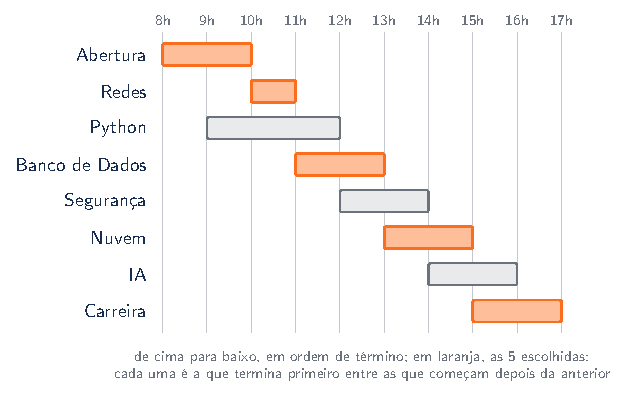
\includegraphics[width=0.85\linewidth,keepaspectratio]{imagens/capitulo-09_atividades.pdf}
\end{center}

Por que essa escolha é segura? Pegue qualquer agenda ótima. Se a primeira palestra dela não for a que termina primeiro, troque-a por esta: como ela termina mais cedo, não pode se sobrepor às seguintes, e a agenda continua com o mesmo número de palestras. Esse argumento de troca é a forma típica de provar que um guloso está correto.

\begin{codigo}
\begin{Verbatim}[breaklines=true, breaksymbolleft={}, fontsize=\footnotesize]
#include <vector>
#include <algorithm>   // sort

struct Palestra {
    string nome;
    int inicio, fim;   // horas
};

// recebe uma cópia: a lista original não é reordenada
vector<Palestra> escolher(vector<Palestra> palestras) {
    sort(palestras.begin(), palestras.end(),
         [](const Palestra &a, const Palestra &b) {
             return a.fim < b.fim;  // termina primeiro
         });
    vector<Palestra> escolhidas;
    int livreDesde = 0;         // fim da última escolhida
    for (const Palestra &p : palestras) {
        if (p.inicio >= livreDesde) {   // não se sobrepõe
            escolhidas.push_back(p);
            livreDesde = p.fim;
        }
    }
    return escolhidas;
}

int main() {
    vector<Palestra> agenda = {
        {"Abertura", 8, 10}, {"Python", 9, 12}, {"Redes", 10, 11},
        {"Banco de Dados", 11, 13}, {"Segurança", 12, 14},
        {"Nuvem", 13, 15}, {"IA", 14, 16}, {"Carreira", 15, 17}};
    for (const Palestra &p : escolher(agenda)) {
        cout << p.nome << " (" << p.inicio << "h-"
             << p.fim << "h)" << endl;
    }
    // Abertura (8h-10h), Redes (10h-11h),
    // Banco de Dados (11h-13h), Nuvem (13h-15h),
    // Carreira (15h-17h)
}
\end{Verbatim}
\end{codigo}

O critério de ordenação é a mesma função anônima (\textit{lambda}) usada no Capítulo 8. Depois da ordenação, que custa $O(n \log n)$, uma única passada escolhe as palestras em $O(n)$. O algoritmo inteiro é $O(n \log n)$.

\subsection{9.3 Árvore geradora mínima: algoritmo de Kruskal}

No Capítulo 6, o Prim construiu a árvore geradora mínima a partir de um vértice, fazendo a árvore crescer aresta por aresta. O \textbf{algoritmo de Kruskal} é outra estratégia gulosa para o mesmo problema, ainda mais direta:

\begin{enumerate}
  \item Ordene todas as arestas da mais leve para a mais pesada.
  \item Percorra as arestas nessa ordem. Aceite cada uma que ligue dois vértices que ainda \textbf{não estão conectados}; recuse as que fechariam um ciclo.
  \item Pare quando tiver $V - 1$ arestas.
\end{enumerate}

\begin{center}
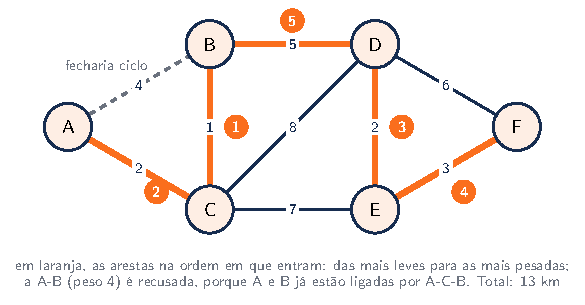
\includegraphics[width=0.8\linewidth,keepaspectratio]{imagens/capitulo-09_kruskal.pdf}
\end{center}

No grafo das cidades, o Kruskal escolhe exatamente as mesmas cinco estradas que o Prim, com o mesmo total de 13 km, mas em outra ordem: o Prim mantém uma única árvore que cresce, enquanto o Kruskal junta vários pedaços soltos que vão se unindo.

\begin{center}
\begin{tabular}{@{}p{0.16\linewidth}p{0.1\linewidth}p{0.64\linewidth}@{}}
\toprule
\rowcolor{headergray}
\tblheader{Aresta} & \tblheader{Peso} & \tblheader{Decisão} \\
\midrule
B-C & 1 & aceita: grupos \{A\} \{B, C\} \{D\} \{E\} \{F\} \\
\rowcolor{rowgray} A-C & 2 & aceita: \{A, B, C\} \{D\} \{E\} \{F\} \\
D-E & 2 & aceita: \{A, B, C\} \{D, E\} \{F\} \\
\rowcolor{rowgray} E-F & 3 & aceita: \{A, B, C\} \{D, E, F\} \\
A-B & 4 & recusada: A e B já estão no mesmo grupo \\
\rowcolor{rowgray} B-D & 5 & aceita: \{A, B, C, D, E, F\}; são 5 arestas, fim \\
\bottomrule
\end{tabular}
\end{center}

\subsubsection{Conjuntos disjuntos (\textit{union-find})}

A pergunta que o Kruskal faz a cada aresta é: ``estes dois vértices já estão no mesmo grupo?''. Percorrer o grafo para responder custaria caro. A estrutura certa é a de \textbf{conjuntos disjuntos} (\textit{union-find}), que guarda grupos que não se misturam e oferece duas operações:

\begin{itemize}
  \item \texttt{raiz(x)}: devolve o representante do grupo de \texttt{x}. Dois elementos estão no mesmo grupo se tiverem a mesma raiz.
  \item \texttt{unir(a, b)}: junta os grupos de \texttt{a} e \texttt{b} em um só.
\end{itemize}

Cada grupo é uma árvore guardada em um vetor \texttt{pai}, como o heap do Capítulo 8: \texttt{pai[x]} é o pai de \texttt{x}, e a raiz é quem é pai de si mesmo. Unir dois grupos é só pendurar a raiz de um embaixo da raiz do outro.

\begin{codigo}
\begin{Verbatim}[breaklines=true, breaksymbolleft={}, fontsize=\footnotesize]
// trecho
class ConjuntosDisjuntos {
private:
    vector<int> pai, tamanho;

public:
    explicit ConjuntosDisjuntos(int n) : pai(n), tamanho(n, 1) {
        for (int i = 0; i < n; i++) pai[i] = i;  // sozinhos
    }

    int raiz(int x) {
        while (pai[x] != x) {
            pai[x] = pai[pai[x]];   // pula para o avô
            x = pai[x];
        }
        return x;
    }

    bool unir(int a, int b) {       // false se já estavam juntos
        a = raiz(a);
        b = raiz(b);
        if (a == b) return false;
        if (tamanho[a] < tamanho[b]) swap(a, b);
        pai[b] = a;                 // menor embaixo do maior
        tamanho[a] += tamanho[b];
        return true;
    }
};
\end{Verbatim}
\end{codigo}

Dois truques mantêm as árvores baixas. Na união, o grupo \textbf{menor} é pendurado no maior, para a altura crescer o mínimo possível. E, a cada \texttt{raiz}, a linha \texttt{pai[x] = pai[pai[x]]} faz cada nó do caminho pular para o avô, encurtando o caminho para as próximas consultas. Com os dois juntos, cada operação custa, na prática, tempo constante.

\begin{codigo}
\begin{Verbatim}[breaklines=true, breaksymbolleft={}, fontsize=\footnotesize]
#include <vector>
#include <tuple>
#include <algorithm>   // sort
#include <utility>     // swap

class ConjuntosDisjuntos {
private:
    vector<int> pai, tamanho;

public:
    explicit ConjuntosDisjuntos(int n) : pai(n), tamanho(n, 1) {
        for (int i = 0; i < n; i++) pai[i] = i;  // sozinhos
    }

    int raiz(int x) {
        while (pai[x] != x) {
            pai[x] = pai[pai[x]];   // pula para o avô
            x = pai[x];
        }
        return x;
    }

    bool unir(int a, int b) {       // false se já estavam juntos
        a = raiz(a);
        b = raiz(b);
        if (a == b) return false;
        if (tamanho[a] < tamanho[b]) swap(a, b);
        pai[b] = a;                 // menor embaixo do maior
        tamanho[a] += tamanho[b];
        return true;
    }
};

using Ligacao = tuple<int, int, int>;   // (peso, de, para)

int kruskal(int n, vector<Ligacao> arestas,
            vector<Ligacao> &escolhidas) {
    sort(arestas.begin(), arestas.end());   // pelo peso primeiro
    ConjuntosDisjuntos grupos(n);
    int total = 0;
    for (const auto &[peso, de, para] : arestas) {
        if (grupos.unir(de, para)) {        // não fecha ciclo
            escolhidas.push_back({peso, de, para});
            total += peso;
            int usadas = static_cast<int>(escolhidas.size());
            if (usadas == n - 1) break;       // árvore completa
        }
    }
    return total;
}

int main() {
    const string NOMES = "ABCDEF";
    enum { A, B, C, D, E, F };
    vector<Ligacao> estradas = {
        {4, A, B}, {2, A, C}, {1, B, C}, {5, B, D}, {8, C, D},
        {7, C, E}, {2, D, E}, {6, D, F}, {3, E, F}};
    vector<Ligacao> escolhidas;
    int total = kruskal(6, estradas, escolhidas);
    for (const auto &[peso, de, para] : escolhidas) {
        cout << NOMES[de] << "-" << NOMES[para] << " ";
    }
    cout << endl;                           // B-C A-C D-E E-F B-D
    cout << "Total: " << total << " km" << endl;   // Total: 13 km
}
\end{Verbatim}
\end{codigo}

Como cada aresta é uma tupla (peso, de, para) e as tuplas são comparadas campo a campo, a \texttt{sort} ordena pelo peso sem precisar de critério próprio. O custo do Kruskal é dominado por essa ordenação: $O(E \log E)$. Ele costuma ser preferido ao Prim quando o grafo já vem como uma lista de arestas, e o Prim, quando vem como lista de adjacência.

\subsection{9.4 Programação dinâmica}

Quando a escolha gulosa não é segura, como no troco com moedas de 4, 3 e 1, é preciso considerar todas as opções. A recursão faz isso naturalmente, mas costuma recalcular a mesma coisa muitas vezes. O exemplo clássico é a sequência de Fibonacci, em que cada termo é a soma dos dois anteriores: 0, 1, 1, 2, 3, 5, 8, 13\ldots{}

\begin{center}
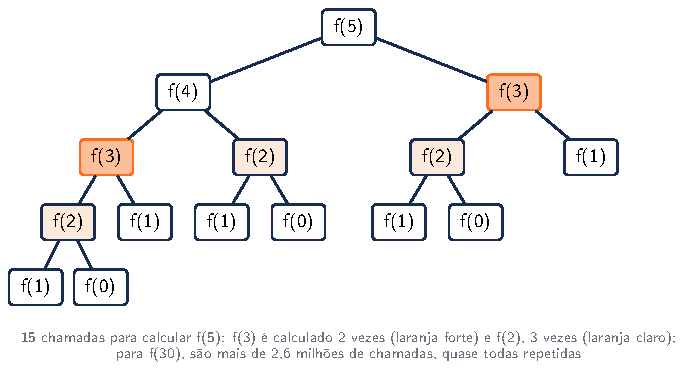
\includegraphics[width=0.9\linewidth,keepaspectratio]{imagens/capitulo-09_fibonacci.pdf}
\end{center}

A recursão direta, \texttt{fib(n) = fib(n - 1) + fib(n - 2)}, abre duas chamadas por nível, e o número de chamadas cresce como $1{,}6^n$. Mas só existem $n + 1$ subproblemas diferentes: \texttt{fib(0)} até \texttt{fib(n)}. Todo o resto é repetição.

A \textbf{programação dinâmica} resolve cada subproblema \textbf{uma única vez} e guarda a resposta em uma tabela. Ela se aplica quando o problema tem \textbf{subestrutura ótima}, como no guloso, e \textbf{subproblemas sobrepostos}: os mesmos subproblemas aparecem muitas vezes. Há dois jeitos de fazer isso:

\begin{itemize}
  \item \textbf{Memorização} (\textit{memoization}, de cima para baixo): mantenha a recursão, mas antes de calcular, veja se a resposta já está guardada; depois de calcular, guarde.
  \item \textbf{Tabulação} (de baixo para cima): preencha a tabela em um laço, dos casos menores para os maiores, de modo que cada posição só dependa de posições já preenchidas.
\end{itemize}

\begin{codigo}
\begin{Verbatim}[breaklines=true, breaksymbolleft={}, fontsize=\footnotesize]
#include <vector>

long long chamadas = 0;

long long fibIngenuo(int n) {
    chamadas++;
    if (n < 2) return n;
    return fibIngenuo(n - 1) + fibIngenuo(n - 2);
}

// memorização: memo[n] == -1 significa "ainda não calculado"
long long fibMemo(int n, vector<long long> &memo) {
    if (n < 2) return n;
    if (memo[n] != -1) return memo[n];       // já sabemos
    memo[n] = fibMemo(n - 1, memo) + fibMemo(n - 2, memo);
    return memo[n];
}

// tabulação: preenche de baixo para cima
long long fibTabela(int n) {
    if (n < 2) return n;
    vector<long long> f(n + 1);
    f[0] = 0;
    f[1] = 1;
    for (int i = 2; i <= n; i++) f[i] = f[i - 1] + f[i - 2];
    return f[n];
}

int main() {
    cout << fibIngenuo(30) << " em " << chamadas
         << " chamadas" << endl;     // 832040 em 2692537 chamadas
    vector<long long> memo(91, -1);
    cout << fibMemo(90, memo) << endl;   // 2880067194370816120
    cout << fibTabela(90) << endl;       // 2880067194370816120
}
\end{Verbatim}
\end{codigo}

As duas versões com tabela fazem $O(n)$ somas. A diferença é brutal: a versão ingênua leva mais de 2,6 milhões de chamadas para \texttt{fib(30)}, e para \texttt{fib(90)} precisaria de cerca de $9 \times 10^{18}$ chamadas, quase 300 anos a um bilhão de chamadas por segundo; as outras calculam \texttt{fib(90)} instantaneamente. Na tabulação, como cada termo só depende dos dois anteriores, dá até para trocar o vetor por duas variáveis e usar memória $O(1)$.

Para resolver um problema com programação dinâmica, siga sempre os mesmos passos:

\begin{enumerate}
  \item \textbf{Defina o subproblema} em palavras: ``\texttt{menor[v]} é o menor número de moedas para formar o valor \texttt{v}''.
  \item \textbf{Escreva a recorrência}: como a resposta de um subproblema se calcula a partir de subproblemas menores.
  \item \textbf{Defina os casos base}: os subproblemas que se resolvem sem recorrência.
  \item \textbf{Escolha a ordem de cálculo}: cada posição da tabela só pode usar posições já calculadas.
  \item \textbf{Reconstrua a solução}, se o problema pedir a escolha e não só o valor: guarde qual opção gerou cada resposta.
\end{enumerate}

\subsection{9.5 Troco com o menor número de moedas}

Voltando ao troco: seja \texttt{menor[v]} o menor número de moedas que somam \texttt{v}. A última moeda usada é alguma moeda \texttt{m}, e o que vem antes dela é um troco ótimo para \texttt{v - m}. Como não sabemos qual é \texttt{m}, testamos todas:

\begin{center}
\texttt{menor[v] = 1 + min(menor[v - m])}, para cada moeda \texttt{m <= v}, \\
com o caso base \texttt{menor[0] = 0}.
\end{center}

Com moedas de 1, 3 e 4, a tabela fica assim. A linha ``última moeda'' guarda a moeda que deu o mínimo, e serve para reconstruir o troco: para 6, a última é 3; para $6 - 3 = 3$, a última também é 3. O troco é $3 + 3$.

\begin{center}
\begin{tabular}{@{}p{0.22\linewidth}p{0.06\linewidth}p{0.06\linewidth}p{0.06\linewidth}p{0.06\linewidth}p{0.06\linewidth}p{0.06\linewidth}p{0.06\linewidth}@{}}
\toprule
\rowcolor{headergray}
\tblheader{valor} & \tblheader{0} & \tblheader{1} & \tblheader{2} & \tblheader{3} & \tblheader{4} & \tblheader{5} & \tblheader{6} \\
\midrule
menor & 0 & 1 & 2 & 1 & 1 & 2 & 2 \\
\rowcolor{rowgray} última moeda & -- & 1 & 1 & 3 & 4 & 1 & 3 \\
\bottomrule
\end{tabular}
\end{center}

\begin{codigo}
\begin{Verbatim}[breaklines=true, breaksymbolleft={}, fontsize=\footnotesize]
#include <vector>

vector<int> trocoMinimo(const vector<int> &moedas, int valor) {
    const int INF = valor + 1;          // mais que o possível
    vector<int> menor(valor + 1, INF), ultima(valor + 1, 0);
    menor[0] = 0;                       // caso base
    for (int v = 1; v <= valor; v++) {  // do menor ao maior
        for (int m : moedas) {
            if (m <= v && menor[v - m] + 1 < menor[v]) {
                menor[v] = menor[v - m] + 1;
                ultima[v] = m;          // para reconstruir
            }
        }
    }
    vector<int> usadas;
    if (menor[valor] == INF) return usadas;   // impossível
    for (int v = valor; v > 0; v -= ultima[v]) {
        usadas.push_back(ultima[v]);
    }
    return usadas;
}

void mostrar(const vector<int> &v) {
    for (int x : v) cout << x << " ";
    cout << endl;
}

int main() {
    mostrar(trocoMinimo({1, 3, 4}, 6));     // 3 3
    mostrar(trocoMinimo({1, 5, 10, 25, 50, 100}, 87));
    // 1 1 10 25 50: as mesmas 5 moedas do guloso
    cout << trocoMinimo({5, 10}, 7).size() << endl;   // 0
}
\end{Verbatim}
\end{codigo}

A programação dinâmica acerta para qualquer conjunto de moedas e também descobre quando o troco é impossível, como 7 centavos só com moedas de 5 e 10. O preço é o custo: $O(\text{valor} \times \text{número de moedas})$, contra o $O(\text{número de moedas usadas})$ do guloso.

\subsection{9.6 O problema da mochila}

Uma pessoa vai acampar com uma mochila que aguenta 7 kg e precisa escolher o que levar. Cada item tem um peso e um valor (a utilidade dele na viagem), e cada um é levado inteiro ou deixado em casa. Qual combinação dá o maior valor sem passar do peso? É o \textbf{problema da mochila 0/1}.

\begin{center}
\begin{tabular}{@{}p{0.3\linewidth}p{0.14\linewidth}p{0.14\linewidth}p{0.26\linewidth}@{}}
\toprule
\rowcolor{headergray}
\tblheader{Item} & \tblheader{Peso} & \tblheader{Valor} & \tblheader{Valor por kg} \\
\midrule
lanterna & 1 kg & 1 & 1,00 \\
\rowcolor{rowgray} cantil & 3 kg & 4 & 1,33 \\
saco de dormir & 4 kg & 5 & 1,25 \\
\rowcolor{rowgray} barraca & 5 kg & 7 & 1,40 \\
\bottomrule
\end{tabular}
\end{center}

A ideia gulosa seria levar primeiro o item com mais valor por quilo: a barraca (5 kg). Depois, só a lanterna cabe, e o total é 8. Mas o cantil com o saco de dormir pesam exatamente 7 kg e valem 9. O guloso falha.

Na programação dinâmica, o subproblema é \texttt{melhor[i][c]}: o maior valor possível usando só os \texttt{i} primeiros itens com uma mochila de capacidade \texttt{c}. Para o item \texttt{i}, só há duas opções: deixá-lo, e a resposta é \texttt{melhor[i - 1][c]}; ou levá-lo, se couber, e a resposta é o valor dele mais \texttt{melhor[i - 1][c - peso]}. A resposta é a maior das duas.

\begin{center}
\begin{tabular}{@{}p{0.27\linewidth}p{0.05\linewidth}p{0.05\linewidth}p{0.05\linewidth}p{0.05\linewidth}p{0.05\linewidth}p{0.05\linewidth}p{0.05\linewidth}p{0.05\linewidth}@{}}
\toprule
\rowcolor{headergray}
\tblheader{capacidade} & \tblheader{0} & \tblheader{1} & \tblheader{2} & \tblheader{3} & \tblheader{4} & \tblheader{5} & \tblheader{6} & \tblheader{7} \\
\midrule
nenhum item & 0 & 0 & 0 & 0 & 0 & 0 & 0 & 0 \\
\rowcolor{rowgray} + lanterna & 0 & 1 & 1 & 1 & 1 & 1 & 1 & 1 \\
+ cantil & 0 & 1 & 1 & 4 & 5 & 5 & 5 & 5 \\
\rowcolor{rowgray} + saco de dormir & 0 & 1 & 1 & 4 & 5 & 6 & 6 & 9 \\
+ barraca & 0 & 1 & 1 & 4 & 5 & 7 & 8 & 9 \\
\bottomrule
\end{tabular}
\end{center}

A resposta está no canto inferior direito: 9. Para saber quais itens levar, refaça o caminho de baixo para cima: se \texttt{melhor[i][c]} for diferente de \texttt{melhor[i - 1][c]}, o item \texttt{i} foi levado, e a capacidade diminui do peso dele.

\begin{codigo}
\begin{Verbatim}[breaklines=true, breaksymbolleft={}, fontsize=\footnotesize]
#include <vector>

struct Item {
    string nome;
    int peso;
    int valor;
};

int mochila(const vector<Item> &itens, int capacidade,
            vector<string> &levados) {
    int n = static_cast<int>(itens.size());
    // melhor[i][c]: maior valor com os i primeiros itens e
    // capacidade c
    vector<vector<int>> melhor(n + 1,
                               vector<int>(capacidade + 1, 0));
    for (int i = 1; i <= n; i++) {
        const Item &item = itens[i - 1];
        for (int c = 0; c <= capacidade; c++) {
            melhor[i][c] = melhor[i - 1][c];      // deixa
            if (item.peso <= c) {                  // ou leva
                int levando = melhor[i - 1][c - item.peso]
                              + item.valor;
                if (levando > melhor[i][c]) {
                    melhor[i][c] = levando;
                }
            }
        }
    }
    for (int i = n, c = capacidade; i > 0; i--) {  // de volta
        if (melhor[i][c] != melhor[i - 1][c]) {
            levados.push_back(itens[i - 1].nome);
            c -= itens[i - 1].peso;
        }
    }
    return melhor[n][capacidade];
}

int main() {
    vector<Item> itens = {{"lanterna", 1, 1},
                          {"cantil", 3, 4},
                          {"saco de dormir", 4, 5},
                          {"barraca", 5, 7}};
    vector<string> levados;
    cout << "Valor: " << mochila(itens, 7, levados) << endl;  // 9
    for (const string &nome : levados) cout << nome << endl;
    // saco de dormir, cantil
}
\end{Verbatim}
\end{codigo}

O custo é $O(n \times \text{capacidade})$, tanto de tempo quanto de memória. Isso é ótimo para capacidades pequenas, mas repare que depende do \textbf{valor} da capacidade, e não só da quantidade de itens: com uma capacidade de um bilhão, a tabela não caberia na memória. Nenhum algoritmo eficiente conhecido resolve a mochila 0/1 em todos os casos.

\begin{destaque}{A mochila fracionária}
Se os itens pudessem ser divididos, como arroz ou água, levando só uma parte, o guloso voltaria a funcionar: leve os itens de maior valor por quilo, e complete a mochila com a fração que couber do próximo. A pequena mudança no enunciado muda a técnica. Antes de escolher entre guloso e programação dinâmica, pergunte se uma escolha feita agora pode atrapalhar escolhas futuras.
\end{destaque}

\subsection{9.7 Guloso ou programação dinâmica?}

\begin{center}
\begin{tabular}{@{}p{0.22\linewidth}p{0.36\linewidth}p{0.32\linewidth}@{}}
\toprule
\rowcolor{headergray}
\tblheader{Técnica} & \tblheader{Como decide} & \tblheader{Exemplos} \\
\midrule
força bruta & testa todas as combinações; sempre certa, quase sempre lenta demais & testar todos os subconjuntos da mochila: $2^n$ \\
\rowcolor{rowgray} guloso & uma escolha por passo, sem voltar atrás; rápido, mas só correto com escolha gulosa & troco com moedas comuns, palestras, Dijkstra, Prim, Kruskal \\
programação dinâmica & considera todas as opções de cada subproblema, mas resolve cada um uma vez & Fibonacci, troco com quaisquer moedas, mochila 0/1 \\
\bottomrule
\end{tabular}
\end{center}

A programação dinâmica aparece em muito mais lugares do que parece. O corretor ortográfico que sugere a palavra mais parecida usa a \textbf{distância de edição}, o menor número de letras a inserir, remover ou trocar para transformar uma palavra em outra. Comparar duas versões de um arquivo, como faz o Git, usa a \textbf{maior subsequência comum}. E comparar sequências de DNA usa variações das duas. Todas são resolvidas com uma tabela preenchida exatamente como as deste capítulo.

\begin{destaque}{Comparando com Python}
Em Python, a memorização vem pronta: o decorador \texttt{@cache}, do módulo \texttt{functools}, guarda o resultado de cada chamada da função e o devolve direto nas chamadas repetidas. Basta colocá-lo antes da versão recursiva, sem mudar mais nada.

\begin{codigo}
\begin{Verbatim}[breaklines=true, breaksymbolleft={}, fontsize=\footnotesize]
from functools import cache

@cache
def fib(n):
    if n < 2:
        return n
    return fib(n - 1) + fib(n - 2)

print(fib(90))   # 2880067194370816120, instantâneo

def troco_minimo(moedas, valor):
    infinito = float('inf')
    menor = [0] + [infinito] * valor
    for v in range(1, valor + 1):
        for m in moedas:
            if m <= v and menor[v - m] + 1 < menor[v]:
                menor[v] = menor[v - m] + 1
    return menor[valor]

print(troco_minimo([1, 3, 4], 6))    # 2
print(troco_minimo([5, 10], 7))      # inf: impossível
\end{Verbatim}
\end{codigo}

Como os inteiros do Python não têm limite, \texttt{fib(200)} também funciona, enquanto o \texttt{long long} do C++ estoura depois de \texttt{fib(92)}. Mas cuidado: com recursões muito fundas, como \texttt{fib(5000)}, o Python atinge o limite de chamadas aninhadas, e a versão com tabela continua sendo a mais segura.
\end{destaque}

\subsection{Erros Comuns}

\begin{itemize}
  \item \textbf{Usar um guloso sem provar que ele funciona.} Uma escolha que parece óbvia, como a maior moeda ou o item mais valioso, pode dar respostas erradas sem nenhum aviso. Procure um contraexemplo pequeno antes de confiar.
  \item \textbf{Ordenar pelo critério errado na seleção de atividades.} Ordenar pelo início ou pela duração parece razoável, mas só a ordem de término garante o máximo.
  \item \textbf{Esquecer a união pelo tamanho ou o encurtamento de caminho.} Sem eles, as árvores do \textit{union-find} podem virar listas, e cada \texttt{raiz} passa a custar $O(n)$.
  \item \textbf{Memorizar sem marcar o que ainda não foi calculado.} Se o valor inicial da tabela (como 0) também puder ser uma resposta válida, a função não sabe distinguir ``calculado'' de ``vazio''. Use um valor impossível, como $-1$.
  \item \textbf{Preencher a tabela na ordem errada.} Na tabulação, cada posição só pode usar posições já preenchidas. Ler uma posição ainda vazia dá uma resposta errada sem nenhum erro aparente.
  \item \textbf{Errar os casos base.} Um \texttt{menor[0]} diferente de 0, ou uma linha ``nenhum item'' que não seja toda de zeros, contamina a tabela inteira.
  \item \textbf{Usar um ``infinito'' que estoura.} Somar 1 a \texttt{numeric\_limits<int>::max()} dá um número negativo. Use um infinito que caiba com folga, como \texttt{valor + 1} no troco.
  \item \textbf{Tentar programação dinâmica com tabelas gigantes.} A tabela da mochila tem $n \times \text{capacidade}$ posições; se a capacidade for enorme, ela não cabe na memória.
\end{itemize}


\end{document}
